% chapter radams_based_archives (fold)
\chapter[Implementations of RADAMS-based radio astronomical archives][RADAMS-based astronomical archives]{Implementations of RADAMS-based radio astronomical archives}
\label{cha:radams_based_archives}
	
	The RADAMS was developed with two main objectives in mind:
	
	\begin{itemize}
		\item Providing a data model for the development of 
		the DSS-63 and IRAM~30m antennas' VO-compliant archives; and
		
		\item Providing the VO with classes for supporting
		radio astronomical observations.
	\end{itemize}
	
	The latter objective was illustrated in the discussions
	of the Curation, Packaging, Policy, and Data Provenance
	parts of the Observation Data Model in
	chapters~\ref{cha:radams_curation_packaging_and_policy} and
	\ref{cha:radams_data_provenance}.
	
	We will devote this chapter to the former objective, and we will
	show how the RADAMS has been used as a blueprint in order to
	create two different VO-compatible radio astronomical archives,
	and how features of each antenna have modified the RADAMS.
	
	\section{The Robledo DSS-63 archive} % (fold)
	\label{sec:the_robledo_dss_63_archive}
		
		The DSS-63 is one of the antennas at the Madrid Deep Space
		Communications Complex. Three Deep Space Communications
		Complexes (DSCCs) where created by NASA in the late 50’s,
		and where located at Canberra (Australia), Madrid (Spain)
		and Goldstone (USA), in order to allow for continuous
		monitoring of the incoming data from Earth-orbiting and
		interplanetary spacecraft missions, as well as radio and
		radar astronomy observations for the exploration of the
		Solar System and the Universe. The combined operation of
		the three DSCCs is what it is known as the Deep Space
		Network (DSN), which is managed by the Jet Propulsion
		Laboratory (JPL).
		
		\begin{figure}[tbp]
			\begin{center}
				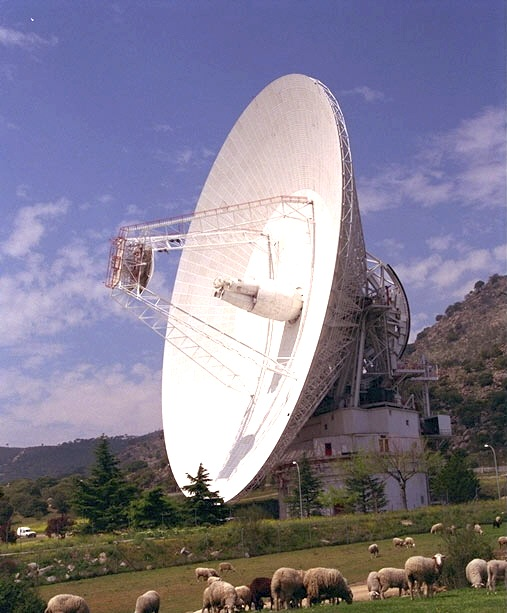
\includegraphics[totalheight=0.45\textheight]
				{fig/DSS-63.jpg}
				\caption[DSS-63 70-meter antenna]
				{
					DSS-63 70-meter antenna at Robledo de Chavela,
					Madrid.
				}
		\label{dss63image}
			\end{center}
		\end{figure}
		
		\begin{table}[tbp]
		\caption[DSS-63 properties, versus other antennas]
		{DSS-63 properties, versus other antennas; values at 22 GHz.}
		\label{dss63comparison}
		\begin{smalltabular}{ccccc} \midrule
				& & \textbf{Aperture} & & \textbf{Sensitivity} \\
		        \textbf{Telescope} & \textbf{Diameter} & \textbf{efficiency
		        ($\mathrm{\eta_a}$)} & \textbf{Resolution} &
		        \textbf{(K/Jy)}\\[4pt] \midrule Effelsberg & 100 m & 29\% & 40’’
		        & 0.8\\ GBT & 100-110 m& 55\% & 34’’ & 1.5\\ Robledo DSS-63 &
		        70 m & 49\% & 42’’ & 0.7\\ 
		\end{smalltabular}
		\end{table}
		
		\begin{table}[tbp]
		\begin{minipage}{\linewidth}
		\caption[Antenna, receiver and spectrometer properties of
		DSS-63]
		{Antenna, receiver and spectrometer properties of DSS-63.}
		\begin{smalltabular}{cl} 
		\multirow{10}*{\minitab[c]{\textbf{Antenna} \\
		\textbf{System}\footnote{HPBW, aperture efficiency, sensitivity and
		pointing accuracy measured at 22GHz, with 40º of elevation}}}
				& \textbf{Name}: Deep Space Station 63 \\
				& \textbf{Diameter}: 70 m \\
				& \textbf{Type}: parabolic Cassegrain \\
				& \textbf{Mount}: azimuth/elevation \\
				& \textbf{Latitude}: 40º 25’ 52’’ N \\
				& \textbf{Longitude}: 04º 14’ 53’’ W \\
				& \textbf{Altitude}: 865.5 m \\
				& \textbf{HPBW}\footnote{Half-Power Beam Width}: 42’’ \\
				& \textbf{Aperture Efficiency ($\eta$)}: 49\% maximum \\
				& \textbf{Sensitivity}: 0.7 K/Jy \\
				& \textbf{Pointing accuracy}: $\leq$ 10'' \\
				\addlinespace\midrule\addlinespace
				
				\multirow{5}*{\minitab[c]{\textbf{K-band} \\
				\textbf{receiver}}} & \textbf{Amplifier type}: cooled HEMT\\
				& \textbf{Frequency range}: 18-26 GHz \\
				& \textbf{Polarization}: LCP\footnote{Left Circular
				Polarisation} or RCP\footnote{Right Circular
				Polarisation}
				(default, LCP) \\
				& \textbf{$\mathbf{T_{sys}}$ (winter)}: 50 K \\
				& \textbf{$\mathbf{T_{sys}}$ (summer)}: 75 K \\
				\addlinespace\midrule\addlinespace

		        \multirow{17}*{\minitab[c]
				{\textbf{Spectrometers}\footnote{The Spaceborne-500
				is the correlator
		        currently in use. It superseded the Spectra-Data,
				the first correlator available in this telescope
				(2001 to 2003), and is no longer in operation.
				The SAO4K, on the other hand, belongs to the
				Smithsonian Astrophysical Observatory, and is used
				for the SAMBA survey.}}} &
		        \textbf{Spaceborne-500}\\ &
		        \textbf{Type}: Digital autocorrelator \\ & \textbf{BW}: 2, 4, 8
		        and 16 MHz\\ & \textbf{Num. channels}: 384\\ &
		        \textbf{Observing mode}: position switching\\
				\addlinespace[3mm]
				
				 &
		        \textbf{Spectra-Data}\\ & \textbf{Type}:
		        Fourier-transform autocorrelator \\ & \textbf{BW}: 1, 2.5, 5
		        and 10 MHz\\ & \textbf{Num. channels}: 256\\ &
		        \textbf{Observing mode}: frequency switching\\
				\addlinespace[3mm]
				&
		        \textbf{SAO4K}\\ & \textbf{Type}: Digital autocorrelator \\ &
		        \textbf{BW}: 400 MHz\\ & \textbf{Num. channels}: 4096\\ &
		        \textbf{Observing mode}: position switching\\ 
		\end{smalltabular}
		\label{dss63properties}
		\end{minipage}
		\end{table}
		
		Each DSCC has at least four operational antennas:

		\begin{itemize}
			\item One 26-meter diameter antenna, originally built
			to support the Apollo missions to the Moon, presently
			used for communicating with Earth-orbiting spacecraft.
			
			 \item One 34-meter diameter high efficiency antenna
			(HEF), designed around a precision-shaped reflector,
			for maximum signal sensitivity.
			
			 \item One 34-meter diameter beam waveguide antenna
			(BWG), based on the HEF design, with five mirrors that
			reflect radio signals along a beam-waveguide tube from
			the antenna vertex to the equipment room, for easier
			maintenance access.
			
			 \item One 70-meter diameter antenna, with the highest
			sensitivity, used for tracking the deepest space
			missions.
		\end{itemize}
		
		In the case of the Madrid DSCC, the 70m antenna is DSS-63,
		whose picture is displayed in figure~\ref{dss63image}.
		Due to their high sensitivity in centimetre wavelengths,
		they can be used to perform astronomical observations,
		when they are not following NASA vehicles .
		
		Of all the time devoted for scientific observations,
		around 3\% of the time at the Canberra and Madrid stations
		(up to 260 hours per year and per antenna) is available to
		Host-Country astronomers. \suppress[Enrique]{The
		organisation responsible for the scheduling of this time at
		Madrid DSCC is the Laboratorio de Astrofísica Espacial y
		Física Fundamental (LAEFF) of the Instituto Nacional de
		Técnica Aeroespacial (INTA), by arrangement with NASA.} The
		organisation responsible for the scheduling of this time at
		Madrid DSCC is the Centro de Astrobiología (INTA-CSIC), by
		arrangement with NASA.
		
		Table~\ref{dss63comparison} compares some properties of
		DSS-63 with those from other astronomically oriented radio
		telescopes, while table~\ref{dss63properties} summarises
		DSS-63 properties of the antenna system, the K-band receiver,
		and the different spectrometers which have been installed at
		the the DSS-63 antenna.
		
		Nowadays, Host Country time at the MDSCC is devoted to
		perform spectroscopic observations at K-band (i.e.,
		wavelengths around 10 cm), with the 70-m DSS-63 antenna.
		In particular, several projects for observing \water{}
		masers have been performed ---see, for intance, Gregorio de
		Monsalvo's thesis~\cite{de-Gregorio-Monsalvo:2006fk}---,
		and the team wished to make those spectroscopic archives
		public.
		
		% subsection spectral_observations_dss63 (fold)
		\subsection{Spectral observations with the DSS-63 antenna}
		\label{sub:spectral_observations_dss63}
			As the main scientific use of the DSS-63 antenna is the
			recollection of spectra, we will describe how
			spectroscopic observations are performed with this
			instrument.
			
			The observing process for a spectrum is as follows:
			
			\begin{description}
				\item[Source selection] First, a target source with
				a medium elevation at the time of observation is
				selected; extreme elevations introduce additional
				pointing errors and/or additional atmospheric
				effects.
				
				\item[Pointing calibrator selection] Once the
				source has been selected, a strong pointing
				calibration source near the target is chosen,
				because minimising antenna motion between pointing
				calibration
				and the actual observation better maintains the
				mirror shape\footnote{Antenna geometry changes
				mostly due to gravitational effects which are
				minimum for changes in azimuth, a much more
				significant for changes in elevation. Large radio
				astronomical antennas are designed following the
				homology principle, so that deformations produce
				changes in focus, so in order to collect the
				maximum flux focus calibrations should be
				performed with sources at the same elevation as
				the source to be observed.}.
				
				\item[Pointing calibration] The antenna will be
				moved up and down in elevation, and clockwise and
				counter-clockwise in cross-elevation, around the
				expected position for the pointing calibrator. As
				the profile for the telescope beam conforms to a
				Gaussian distribution, the data can be fitted with
				a Gaussian, and the pointing error adjusted by
				comparison between the expected position of the
				calibrator, and the fitted maximum flux position.
				This correction will be applied to the coordinates
				where the source is expected to be.
				
				\item[Focus calibration] The same calibrator can be
				used to calibrate the focus of the instrument,
				defined as the position of the secondary mirror
				that maximises the power collected by the
				instrument. Again, the profile for the focus, when
				the mirror is moved along its axis, is assumed to
				be Gaussian, and the fit for the maximum
				provides the focus.
				
				\item[On/Off source observation] Both the source
				and a nearby position with no emissions have to be
				observed, in order to discriminate the contribution
				from the instrument. This is performed either by
				changing the position of the antenna (position
				switching), or by moving the secondary mirror in
				such a way that the main feed is focused on a
				different region of the sky, with no radio sources
				(wobbler switching). Another possibility is to
				compare the power of the emission from the same
				source at slightly different frequencies, assuming
				that the antenna and atmospheric noise does not
				change with this frequency switch (frequency
				switching). In the case of the DSS-63, on/off
				observations are performed either by position
				switching or frequency switching.
				
				\item[Atmospheric corrections] The amount of energy
				received by the instrument depends strongly on
				weather conditions, and on the length of the path
				of the signal through the atmosphere. In
				particular, at cm wavelengths the amount of water
				vapour in the atmosphere is the major contributor
				to atmospheric opacity (a quantity that is
				proportional to the probability of a photon being
				absorbed after travelling a given length in the
				atmosphere). Measurements of opacity at different
				elevations (tipping curves, or skydips), which
				correspond to different air masses (a measure of
				the amount of atmospheric gas in the line of sight
				of the instrument), are used to fit a curve that
				provides the atmospheric opacity\footnote{See
				section 7.2 in \emph{Tools of radio
				astronomy}~\cite{2004tra..book.....R} for
				details.}. This is usually
				done at DSS-63 once per observing session and
				frequency setup.
			\end{description}
			
			There are other corrections and calibrations to
			consider, but most of them can be obtained from typical
			values for the instrument and particular configuration,
			and do not contribute to illustrate the observing
			process with the DSS-63 antenna.
			
			 Of particular interest will be parameters such as
			system temperature ($\mathrm{T_{sys}}$), main beam
			solid angle ($\mathrm{\Omega_{mb}}$), aperture
			efficiency ($\mathrm{\eta_a}$), and the antenna
			temperature scale.
			
			 The data output of the correlator is a 384-sample
			autocorrelation function, which by means of the Fourier
			transform (Discrete Fourier Transform, in this case)
			provides a function proportional to the power spectrum
			of the source\footnote{See section 4.1.2 of \emph{Tools
			of Radio Astronomy}~\cite{2004tra..book.....R} for the
			derivation.}. The post-processing of the observation,
			together with the calibration procedures, will allow us
			to determine the actual spectrum scale, and frequencies
			for the salient features of the spectrum.
			
		% subsection spectral_observations_dss63 (end)
		
		\subsection{Archive requirements} % (fold)
		\label{sub:archive_requirements_dss63}
			
			The archive for the DSS-63 antenna, then, is an
			archive for single-point spectroscopic observations.
			The particular requirements for the archive were:
			
			\begin{description}
				\item[Support for two single-point modes] The
				DSS-63 antenna archive would hold, as per the
				initial specification, only single-point on-off
				spectra using frequency switching, or
				single-point continuum measurements.
				
				\item[VO spectral access services] The main data
				products of the archive are spectra, which are
				supported by the Spectrum Data Model (incorporated
				in the RADAMS, as we have seen), and continuum
				measurements, which are considered to be one-point,
				wide-band spectra, similar to photometric data
				points in the visible band. A SSAP service will
				be implemented on top of the database, as well
				as a ConeSearch on the Scans table.
				
				\item[Web access interface] The web access
				interface would use the same infrastructure needed
				for the SSAP service, but providing a VO compatible
				spectral web-service, instead of using web forms.
				
				\item[No modification to the instrument control
				system] All of the information stored in the
				archive should be available either from ingestion
				of the FITS files, or by harvesting the observation
				logs and control system output, but nothing should
				be added to the instrument control system. This is
				both a precautionary measure, so that we do not
				interfere with the telescope, but also works for
				making the project self-contained: tasks can be
				performed without need for external developers to
				modify another piece of software.
				
				\item[Simple data access policy] The MSDCC data
				standard access policy is the
				straightforward NRAO policy: after 18 months, data
				are available to the public. However, as all data
				to be provided by these archive are older than that,
				there is no actual Policy module for this archive.
			\end{description}
			
		% subsection archive_requirements_dss63 (end)
		
		\subsection{Archive architecture} % (fold)
		\label{sub:archive_architecture_dss63}
			
			\begin{figure}[tbp]
				\begin{center}
					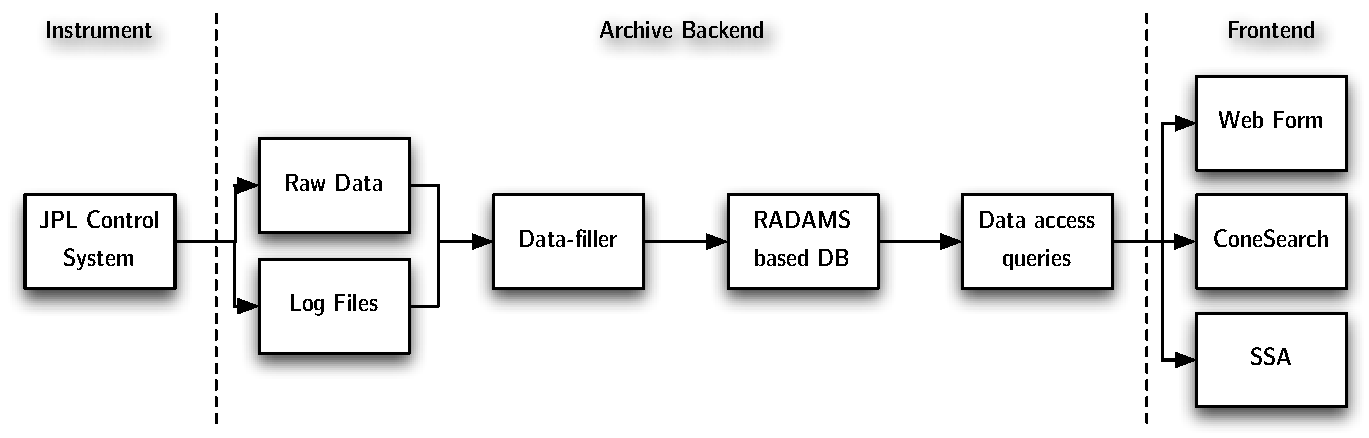
\includegraphics[width=\textwidth]
					{fig/DSS63_ArchiveArchitecture.pdf}
				\end{center}
				\caption[High level, layered architecture for the
				Robledo Archive]
				{High level, layered architecture for the Robledo
				Archive. Dotted lines represent the logical
				separation between layers. Arrows represent data
				flow between sub-systems. Communications between
				layers are confined to the communications
				established between interfacing components.}
				\label{figDss63ArchiveArchitecture}
			\end{figure}
			
			With the requirements above, a layered
			architecture for the archive was devised where each
			layer correspond to a different subsystem:
			
			\begin{description}
				\item[Instrument] With regards to the archive, the
				Instrument is represented by the Instrument Control
				System, which provides the links to observational
				data and configuration metadata.
				

				\item[Archive Backend] The backend of the archive 
				(not to be confused with any of the instrument’s
				back-ends) is the module responsible for database
				and metadata access and maintenance. Includes the
				creation of entries in the database from the Raw
				data and observation log files, and the queries for
				supporting different query interfaces.
				
				
				\item[Frontend] This is the actual accessible layer
				for human-computer or computer-computer interaction
				with the Archive Backend, using either a web form
				interface, or VO services such as ConeSearch for
				observation logs, and SSA for obtaining actual
				spectra.
			\end{description}
			
			
			Figure~\ref{figDss63ArchiveArchitecture} shows that
			layered organisation, and how each layer maintains a
			single point of interaction with the next.
			
			\suppress[Juande]{
			One of the most important parts of the system is what
			in that figure is called the Archive Infrastructure,
			which contains the methods for accessing Instrument
			logs, the database following the RADAMS data model
			for the metadata, and the raw data storage.
			
			One of the sub-modules in the Archive Infrastructure
			module is the Data-filler, which waits for messages
			from the Instrument (in the form of entries on the
			observation log), and ingests them into the database,
			with links to the raw data storage.}
			
			We have detailed several subsystems within the 
			Archive Backend: the Data-filler, which waits for messages
			from the Instrument (in the form of entries on the
			observation log), ingesting them into the database,
			with links to the raw data storage; the database itself,
			which as we will see conforms to the RADAMS; and
			the archive queries to support the different use cases.
			
			Apart from the automatic operation mode, the Data-filler
			can
			also be launched on its own, providing it with a set of
			FITS files to ingest, and the observing logs making
			reference to those FITS files.
			
			For this archive, we have developed the complete Archive
			Backend, including the database implementation, which
			has been developed using the
			Django\urlnote{http://www.djangoproject.com/}
			Python-based development framework. The database being
			used is Oracle, as per CAB prescriptions, and the user
			interface and VO data access modules built on top of
			the RADAMS will be developed by the SVO members of the
			LAEFF.
			
			An interesting feature of the Archive Backend for the
			DSS-63 antenna, which has been also implemented for
			the IRAM~30m, is the way VO-related metadata (UCDs,
			UTypes, and other IVOA vocabularies) are provided 
			to the Data access queries. We will describe that
			mechanism when discussing the implementation details
			of the IRAM~30m archive.
			
		% subsection archive_architecture_dss63 (end)
		
		\subsection{RADAMS implementation} % (fold)
		\label{sub:radams_implementation_dss63}
			\newcommand{\dsssixtythreesqlurl}
			{http://www.iaa.es/~jdsant/thesis/dss63-sourceDM-v0_5.sql}
			
			Figure~\ref{fig:fig_DSS63-data-model} shows the
			different database tables and their
			relationships\footnote {The complete \texttt{.sql} file
			implementing tables and relationships can be found
			at:\\ \url{\dsssixtythreesqlurl}.} used for the actual
			implementation of the DSS-63 archive.
			
			If we compare that figure with the high-level overview
			of the RADAMS ---figure~\ref{RADAMSHLoverview}---, we
			can see that in the archive implementation there are
			many more dependencies on the Observation or ObsData
			related tables in the archive database than those shown
			for the RADAMS.
			
			That is so because we need to be able to perform
			different direct relationships with scans, as different
			search capabilities would be unfeasible if the whole
			dependency tree had to be traversed. However, in order
			to describe an observation (scan) or a set of
			associated scans, those additional dependencies are
			implicit, and need not be stated, as is the case with
			the high-level RADAMS data model.
			
			\suppress[Juande]
			{listing~\ref{lst:dss63-sql} shows the beginning of the
			SQL statements which define the data model and table
			layout, and provide a link to the complete SQL file.}
			
			\begin{figure}[tbp]
				\centering
					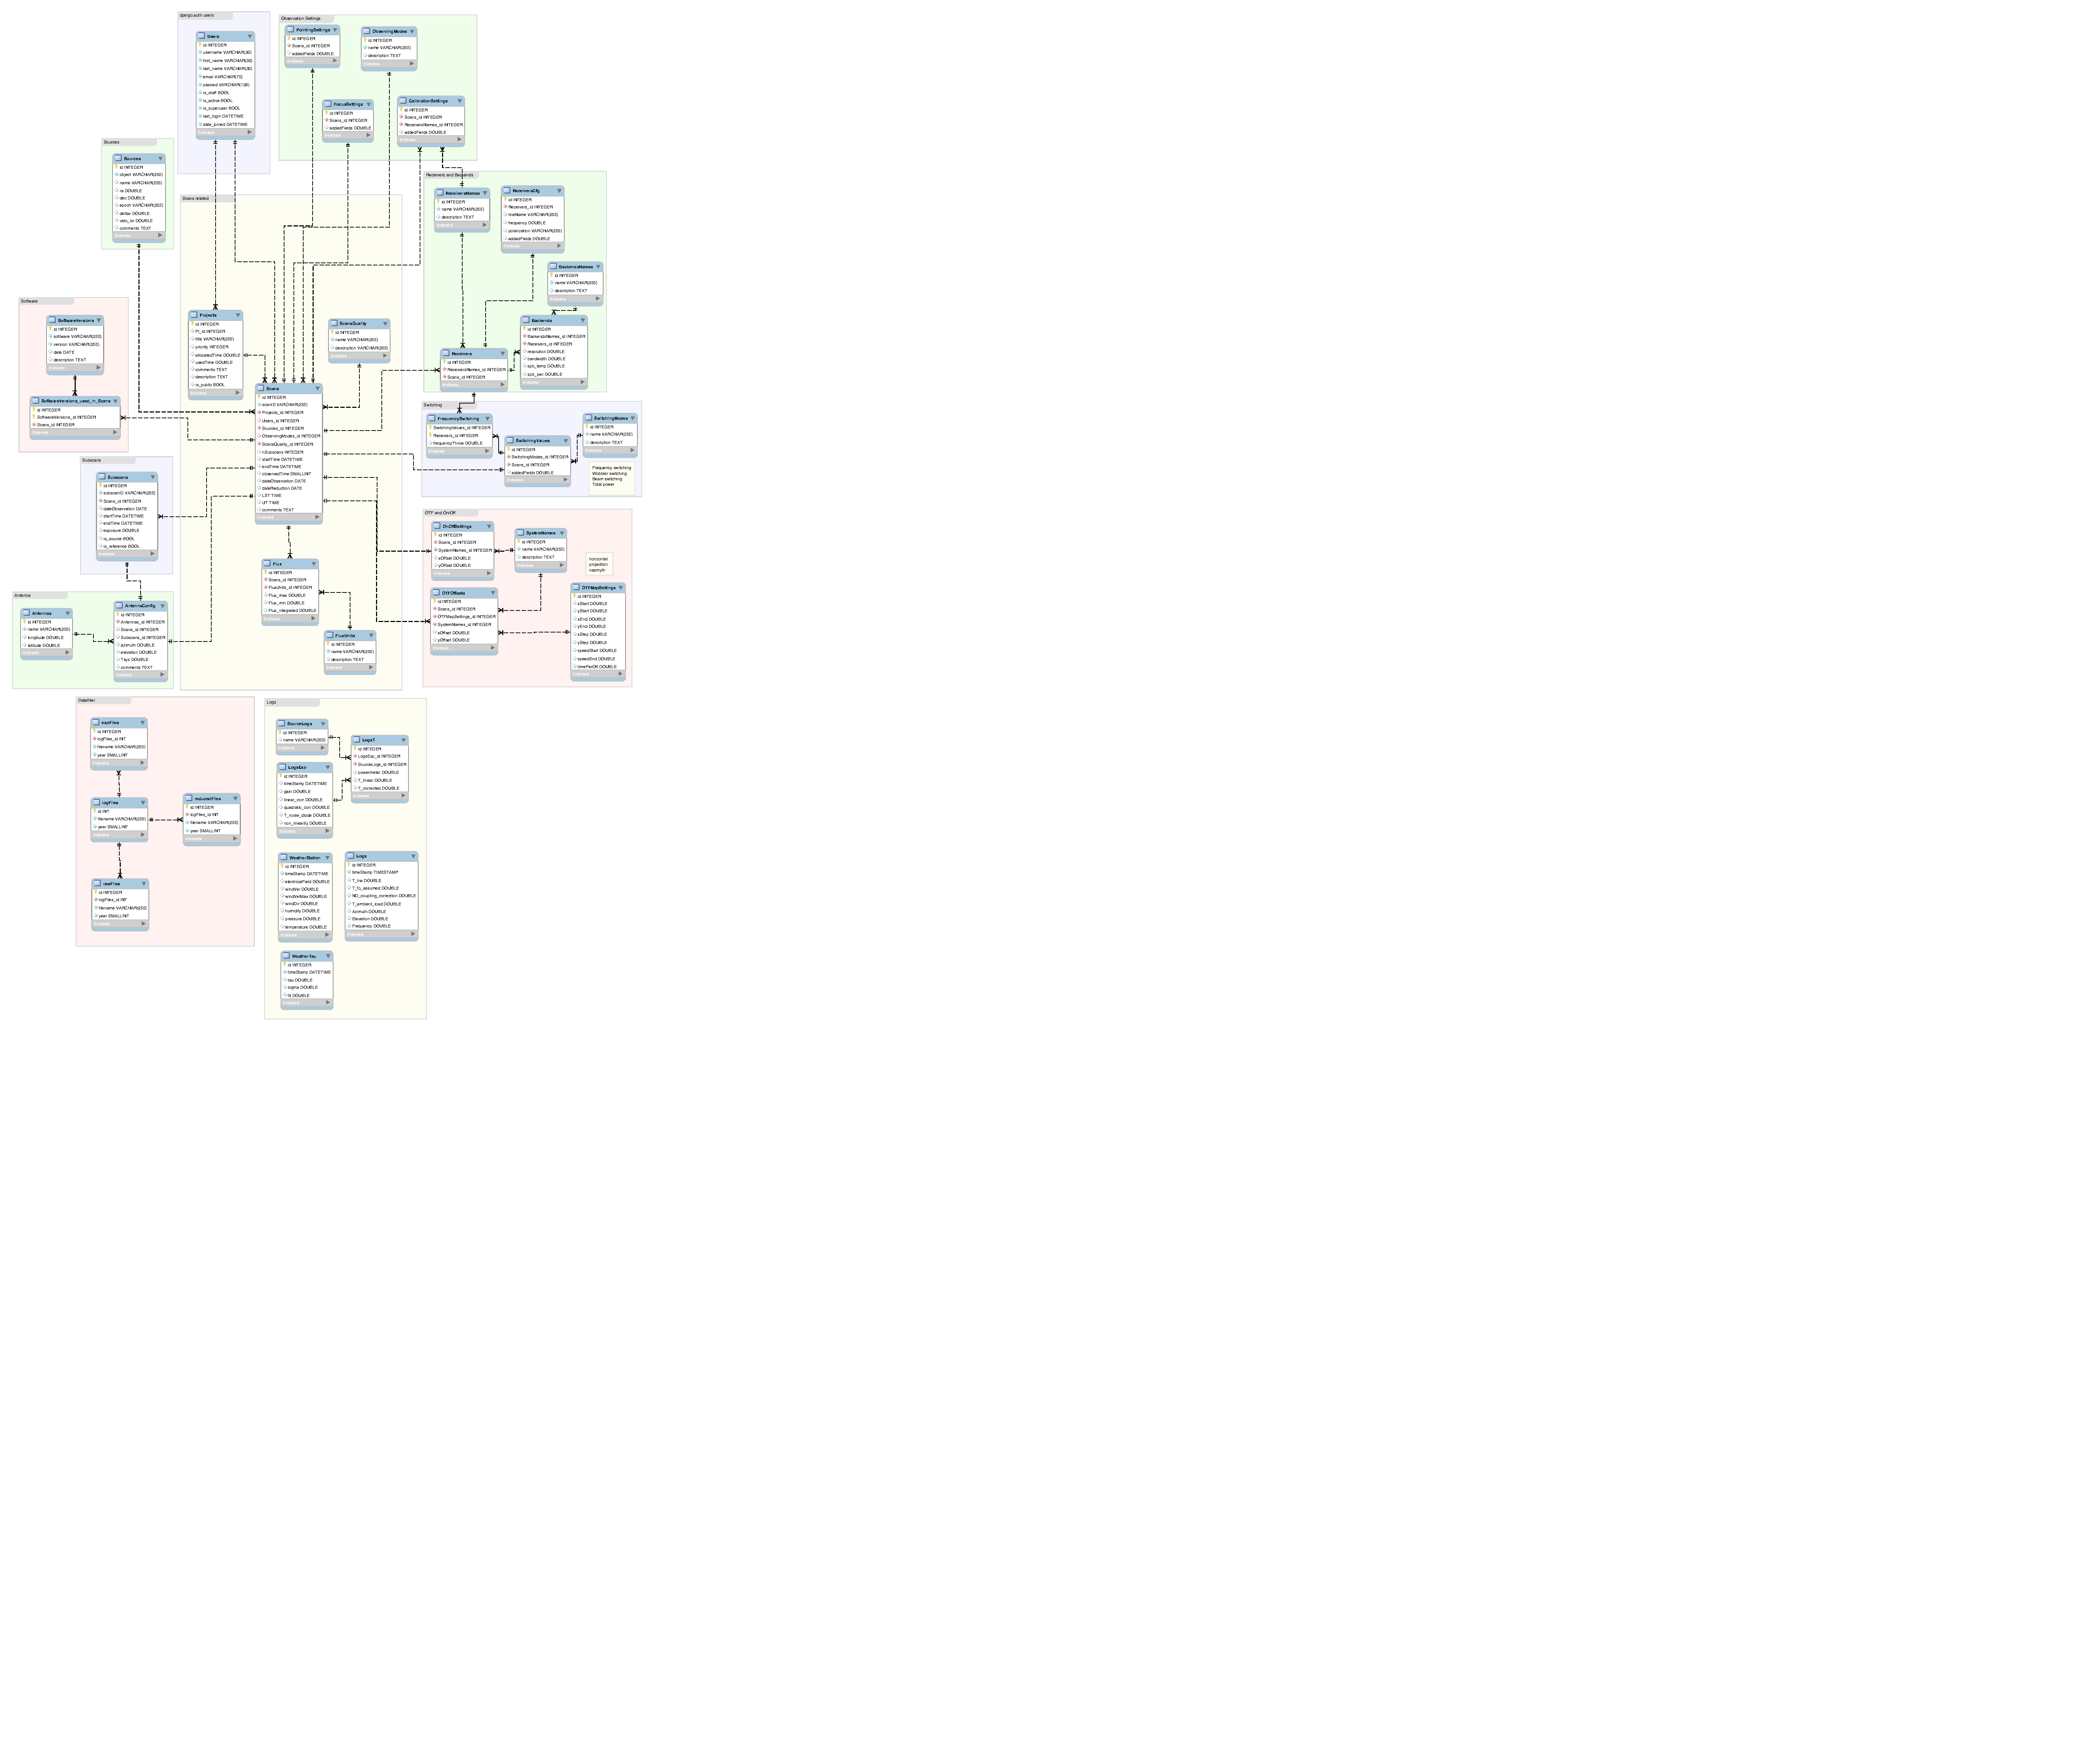
\includegraphics[totalheight=1.1\textheight]
					{fig/DSS63-dm.pdf}
				\caption[Implementation of the data model for the
				DSS-63 archive]
				{
					Implementation of the data model for the
					DSS-63 archive, generated from the actual
					SQL \method{CREATE TABLE} statements.
				}
				\label{fig:fig_DSS63-data-model}
			\end{figure}
			
			The Scan object is the cornerstone for
			all observations, as we discussed in
			section~\ref{subObsDataCharacterisation}. From the
			Scan entity, all other relationships derive, except
			for those having to do with the Data-filler
			configuration ---which are themselves outside of the
			scope of the RADAMS---, and data which are related to
			Scans only by simultaneity, as is the case for
			weather station readings, whose only relation to
			Scans is their timestamp.
			
			Sources implements a very simplified Target data model.
			
			Project metadata is directly related to observations
			as part of the Curation data model, and to Users.
			Project and Users would be used by the Policy algorithm
			if DSS-63 archive's policy were not fixed, as
			previously stated.
			
			The Observations Settings, Receivers and Backends,
			Switching, Antenna and observation Settings are the
			tables supporting
			the Provenance.Instrument data model. Many of the tables
			are tables for instrument codes, or instrument setting
			codes.
			
			The major mismatch between the RADAMS data model
			(developed for VO data query, and data description)
			and the actual data stored in the database (retrieved
			from the data available through the FITS file headers,
			and from the instrument control system), is found in
			the Characterisation data model: metadata such as
			spatial resolution, spectral resolution, et cetera,
			are derived from the values of the observation
			settings, and are not to be stored with the database,
			but will be, instead, generated on the fly by the
			VO interfaces. We will revisit this peculiarity when
			describing the IRAM~30m archive database and its
			relationship to the RADAMS.
			
			\begin{figure}[tbp]
				\centering
					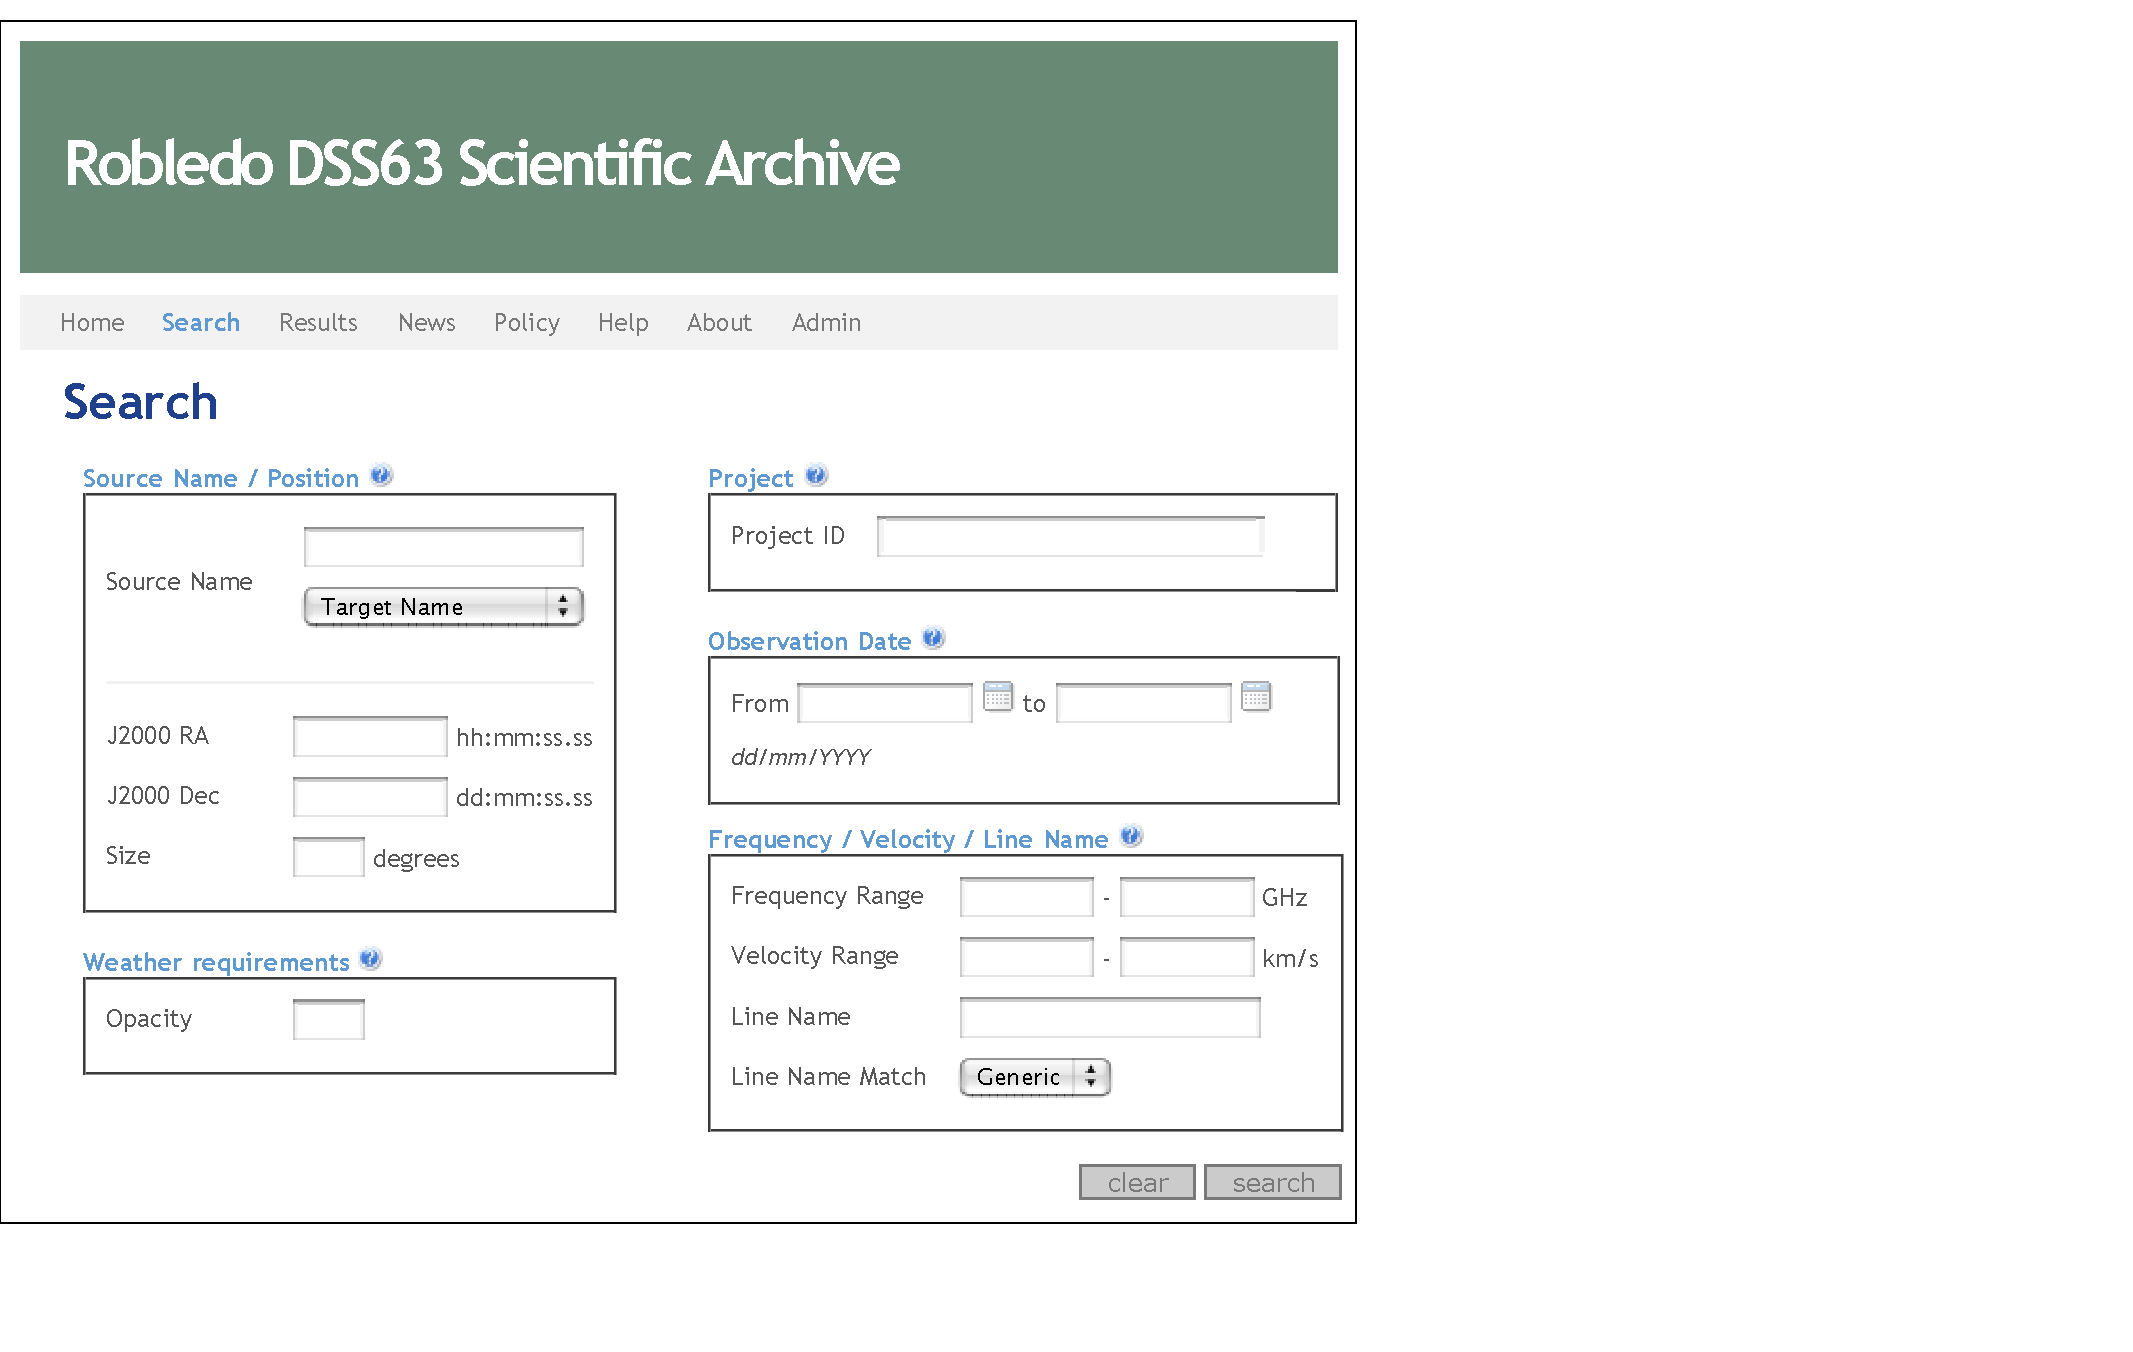
\includegraphics[width=\textwidth]
					{fig/DSS63_searchForm.pdf}
				\caption{
					Prototype search form for the DSS-63 archive.
				}
				\label{fig:fig_DSS63_searchForm}
			\end{figure}
			
			The prototype web form interface to the archive
			can bee seen in figure~\ref{fig:fig_DSS63_searchForm},
			where the Target data model (and CharDM Spatial axis)
			is queried by the Source name and position search box,
			the Project search box queries Observation metadata,
			Observation date is related to the CharDM in the
			Temporal axis, and Frequency/Velocity and Line names
			perform their searches on the CharDM Spectral and
			Velocity axes.
			
			\suppress[Juande]{
			\lstinputlisting[
				language=SQL,
				caption={[SQL statements for Robledo data model]
				First SQL statements for Robledo data model.
				The complete SQL file can be downloaded from the
				following link:\\
				\url{\dsssixtythreesqlurl}
				},
				label=lst:dss63-sql,
				firstline=1,
				lastline=65,
				float=tbp
			]
			{listing/dss63-sourceDM-v0_5.sql}
			
			In order to be able to compare the RADAMS with the
			actual SQL files, the following pages are devoted to
			show all tables and attributes, with data types,
			ability to hold null files and default values.
			
			Table primary keys are in \textbf{\emph{bold italics}},
			while unique fields are in \textbf{bold}.
			
			\clearpage
			
			% phpMyAdmin LaTeX Dump
% version 2.11.7.1
% http://www.phpmyadmin.net
%
% Servidor: localhost
% Tiempo de generación: 25-03-2009 a las 22:24:51
% Versión del servidor: 5.0.41
% Versión de PHP: 5.2.6
% 
% Base de datos: 'dss63'
% 

%
% Estructura: antennaconfig
%
 \begin{longtable}{lcccl}
 
 \caption{Structure of table \texttt{antennaconfig}} \label{tab:antennaconfig-structure} \\
 \textbf{Field} & \textbf{Type} & \textbf{Null} & \textbf{Default}  \\ \midrule
\endfirsthead
 \caption*{Structure of table \texttt{antennaconfig} (continued)} \\ 
 \addlinespace \textbf{Field} & \textbf{Type} & \textbf{Null} & \textbf{Default}  \\ \midrule \endhead \endfoot 
\textbf{\textit{id}} & int(11) & Yes & NULL \\ \addlinespace 
Antennas\_id & int(11) & Yes &  \\ \addlinespace 
Scans\_id & int(11) & Yes & NULL \\ \addlinespace 
Subscans\_id & int(11) & Yes & NULL \\ \addlinespace 
azimuth & double & Yes & NULL \\ \addlinespace 
elevation & double & Yes & NULL \\ \addlinespace 
Tsys & double & Yes & NULL \\ \addlinespace 
comments & longtext & Yes &  \\ 
 \end{longtable}

%
% Estructura: antennas
%
 \begin{longtable}{lcccl}
 
 \caption{Structure of table \texttt{antennas}} \label{tab:antennas-structure} \\
 \addlinespace \textbf{Field} & \textbf{Type} & \textbf{Null} & \textbf{Default}  \\ \midrule
\endfirsthead
 \caption*{Structure of table \texttt{antennas} (continued)} \\ 
 \addlinespace \textbf{Field} & \textbf{Type} & \textbf{Null} & \textbf{Default}  \\ \midrule \endhead \endfoot 
\textbf{\textit{id}} & int(11) & Yes & NULL \\ \addlinespace 
name & varchar(255) & Yes &  \\ \addlinespace 
longitude & double & Yes & NULL \\ \addlinespace 
latitude & double & Yes & NULL \\ 
\end{longtable}

%
% Estructura: backends
%
 \begin{longtable}{lcccl}
 
 \caption{Structure of table \texttt{backends}} \label{tab:backends-structure} \\
 \addlinespace \textbf{Field} & \textbf{Type} & \textbf{Null} & \textbf{Default}  \\ \midrule
\endfirsthead
 \caption*{Structure of table \texttt{backends} (continued)} \\ 
 \addlinespace \textbf{Field} & \textbf{Type} & \textbf{Null} & \textbf{Default}  \\ \midrule \endhead \endfoot 
\textbf{\textit{id}} & int(11) & Yes & NULL \\ \addlinespace 
BackendsNames\_id & int(11) & Yes &  \\ \addlinespace 
Receivers\_id & int(11) & Yes &  \\ \addlinespace 
resolution & double & Yes & NULL \\ \addlinespace 
bandwidth & double & Yes & NULL \\ \addlinespace 
spb\_temp & double & Yes & NULL \\ \addlinespace 
spb\_pwr & double & Yes & NULL \\ 
  \end{longtable}

%
% Estructura: backendsnames
%
 \begin{longtable}{lcccl}
 
 \caption{Structure of table \texttt{backendsnames}} \label{tab:backendsnames-structure} \\
 \addlinespace \textbf{Field} & \textbf{Type} & \textbf{Null} & \textbf{Default}  \\ \midrule
\endfirsthead
 \caption*{Structure of table \texttt{backendsnames} (continued)} \\ 
 \addlinespace \textbf{Field} & \textbf{Type} & \textbf{Null} & \textbf{Default}  \\ \midrule \endhead \endfoot 
\textbf{\textit{id}} & int(11) & Yes & NULL \\ \addlinespace 
name & varchar(255) & Yes &  \\ \addlinespace 
description & longtext & Yes &  \\ 
  \end{longtable}

%
% Estructura: calibrationsettings
%
 \begin{longtable}{lcccl}
 
 \caption{Structure of table \texttt{calibrationsettings}} \label{tab:calibrationsettings-structure} \\
 \addlinespace \textbf{Field} & \textbf{Type} & \textbf{Null} & \textbf{Default}  \\ \midrule
\endfirsthead
 \caption*{Structure of table \texttt{calibrationsettings} (continued)} \\ 
 \addlinespace \textbf{Field} & \textbf{Type} & \textbf{Null} & \textbf{Default}  \\ \midrule \endhead \endfoot 
\textbf{\textit{id}} & int(11) & Yes & NULL \\ \addlinespace 
Scans\_id & int(11) & Yes &  \\ \addlinespace 
Receivers\_id & int(11) & Yes &  \\ 
  \end{longtable}


%
% Estructura: expfiles
%
 \begin{longtable}{lcccl}
 
 \caption{Structure of table \texttt{expfiles}} \label{tab:expfiles-structure} \\
 \addlinespace \textbf{Field} & \textbf{Type} & \textbf{Null} & \textbf{Default}  \\ \midrule
\endfirsthead
 \caption*{Structure of table \texttt{expfiles} (continued)} \\ 
 \addlinespace \textbf{Field} & \textbf{Type} & \textbf{Null} & \textbf{Default}  \\ \midrule \endhead \endfoot 
\textbf{\textit{id}} & int(11) & Yes & NULL \\ \addlinespace 
logFiles\_id & int(11) & Yes &  \\ \addlinespace 
\textbf{filename} & varchar(255) & Yes &  \\ \addlinespace 
year & smallint(6) & Yes &  \\ 
  \end{longtable}

%
% Estructura: flux
%
 \begin{longtable}{lcccl}
 
 \caption{Structure of table \texttt{flux}} \label{tab:flux-structure} \\
 \addlinespace \textbf{Field} & \textbf{Type} & \textbf{Null} & \textbf{Default}  \\ \midrule
\endfirsthead
 \caption*{Structure of table \texttt{flux} (continued)} \\ 
 \addlinespace \textbf{Field} & \textbf{Type} & \textbf{Null} & \textbf{Default}  \\ \midrule \endhead \endfoot 
\textbf{\textit{id}} & int(11) & Yes & NULL \\ \addlinespace 
Scans\_id & int(11) & Yes &  \\ \addlinespace 
FluxUnits\_id & int(11) & Yes &  \\ \addlinespace 
Flux\_max & double & Yes & NULL \\ \addlinespace 
Flux\_min & double & Yes & NULL \\ \addlinespace 
Flux\_integrated & double & Yes & NULL \\ 
  \end{longtable}

%
% Estructura: fluxunits
%
 \begin{longtable}{lcccl}
 
 \caption{Structure of table \texttt{fluxunits}} \label{tab:fluxunits-structure} \\
 \addlinespace \textbf{Field} & \textbf{Type} & \textbf{Null} & \textbf{Default}  \\ \midrule
\endfirsthead
 \caption*{Structure of table \texttt{fluxunits} (continued)} \\ 
 \addlinespace \textbf{Field} & \textbf{Type} & \textbf{Null} & \textbf{Default}  \\ \midrule \endhead \endfoot 
\textbf{\textit{id}} & int(11) & Yes & NULL \\ \addlinespace 
name & varchar(255) & Yes &  \\ \addlinespace 
description & longtext & Yes &  \\ 
  \end{longtable}

%
% Estructura: focussettings
%
 \begin{longtable}{lcccl}
 
 \caption{Structure of table \texttt{focussettings}} \label{tab:focussettings-structure} \\
 \addlinespace \textbf{Field} & \textbf{Type} & \textbf{Null} & \textbf{Default}  \\ \midrule
\endfirsthead
 \caption*{Structure of table \texttt{focussettings} (continued)} \\ 
 \addlinespace \textbf{Field} & \textbf{Type} & \textbf{Null} & \textbf{Default}  \\ \midrule \endhead \endfoot 
\textbf{\textit{id}} & int(11) & Yes & NULL \\ \addlinespace 
Scans\_id & int(11) & Yes &  \\ 
  \end{longtable}

%
% Estructura: frequencyswitching
%
 \begin{longtable}{lcccl}
 
 \caption{Structure of table \texttt{frequencyswitching}} \label{tab:frequencyswitching-structure} \\
 \addlinespace \textbf{Field} & \textbf{Type} & \textbf{Null} & \textbf{Default}  \\ \midrule
\endfirsthead
 \caption*{Structure of table \texttt{frequencyswitching} (continued)} \\ 
 \addlinespace \textbf{Field} & \textbf{Type} & \textbf{Null} & \textbf{Default}  \\ \midrule \endhead \endfoot 
\textbf{\textit{id}} & int(11) & Yes & NULL \\ \addlinespace 
SwitchingValues\_id & int(11) & Yes &  \\ \addlinespace 
Receivers\_id & int(11) & Yes &  \\ \addlinespace 
frequencyThrow & double & Yes & NULL \\ 
  \end{longtable}

%
% Estructura: logfiles
%
 \begin{longtable}{lcccl}
 
 \caption{Structure of table \texttt{logfiles}} \label{tab:logfiles-structure} \\
 \addlinespace \textbf{Field} & \textbf{Type} & \textbf{Null} & \textbf{Default}  \\ \midrule
\endfirsthead
 \caption*{Structure of table \texttt{logfiles} (continued)} \\ 
 \addlinespace \textbf{Field} & \textbf{Type} & \textbf{Null} & \textbf{Default}  \\ \midrule \endhead \endfoot 
\textbf{\textit{id}} & int(11) & Yes & NULL \\ \addlinespace 
\textbf{filename} & varchar(255) & Yes &  \\ \addlinespace 
year & smallint(6) & Yes &  \\ 
  \end{longtable}

%
% Estructura: logs
%
 \begin{longtable}{lcccl}
 
 \caption{Structure of table \texttt{logs}} \label{tab:logs-structure} \\
 \addlinespace \textbf{Field} & \textbf{Type} & \textbf{Null} & \textbf{Default}  \\ \midrule
\endfirsthead
 \caption*{Structure of table \texttt{logs} (continued)} \\ 
 \addlinespace \textbf{Field} & \textbf{Type} & \textbf{Null} & \textbf{Default}  \\ \midrule \endhead \endfoot 
\textbf{\textit{id}} & int(11) & Yes & NULL \\ \addlinespace 
\textbf{timeStamp} & datetime & Yes &  \\ \addlinespace 
T\_lna & double & Yes & NULL \\ \addlinespace 
T\_fo\_assumed & double & Yes & NULL \\ \addlinespace 
ND\_coupling\_correction & double & Yes & NULL \\ \addlinespace 
T\_ambient\_load & double & Yes & NULL \\ \addlinespace 
Azimuth & double & Yes & NULL \\ \addlinespace 
Elevation & double & Yes & NULL \\ \addlinespace 
Frequency & double & Yes & NULL \\ 
  \end{longtable}

%
% Estructura: logsexp
%
 \begin{longtable}{lcccl}
 
 \caption{Structure of table \texttt{logsexp}} \label{tab:logsexp-structure} \\
 \addlinespace \textbf{Field} & \textbf{Type} & \textbf{Null} & \textbf{Default}  \\ \midrule
\endfirsthead
 \caption*{Structure of table \texttt{logsexp} (continued)} \\ 
 \addlinespace \textbf{Field} & \textbf{Type} & \textbf{Null} & \textbf{Default}  \\ \midrule \endhead \endfoot 
\textbf{\textit{id}} & int(11) & Yes & NULL \\ \addlinespace 
\textbf{timeStamp} & datetime & Yes &  \\ \addlinespace 
gain & double & Yes & NULL \\ \addlinespace 
linear\_corr & double & Yes & NULL \\ \addlinespace 
quadratic\_corr & double & Yes & NULL \\ \addlinespace 
T\_noise\_diode & double & Yes & NULL \\ \addlinespace 
non\_linearity & double & Yes & NULL \\ 
  \end{longtable}

%
% Estructura: logst
%
 \begin{longtable}{lcccl}
 
 \caption{Structure of table \texttt{logst}} \label{tab:logst-structure} \\
 \addlinespace \textbf{Field} & \textbf{Type} & \textbf{Null} & \textbf{Default}  \\ \midrule
\endfirsthead
 \caption*{Structure of table \texttt{logst} (continued)} \\ 
 \addlinespace \textbf{Field} & \textbf{Type} & \textbf{Null} & \textbf{Default}  \\ \midrule \endhead \endfoot 
\textbf{\textit{id}} & int(11) & Yes & NULL \\ \addlinespace 
SourceLogs\_id & int(11) & Yes &  \\ \addlinespace 
LogsExp\_id & int(11) & Yes &  \\ \addlinespace 
powermeter & double & Yes & NULL \\ \addlinespace 
T\_linear & double & Yes & NULL \\ \addlinespace 
T\_corrected & double & Yes & NULL \\ 
  \end{longtable}

%
% Estructura: observingmodes
%
 \begin{longtable}{lcccl}
 
 \caption{Structure of table \texttt{observingmodes}} \label{tab:observingmodes-structure} \\
 \addlinespace \textbf{Field} & \textbf{Type} & \textbf{Null} & \textbf{Default}  \\ \midrule
\endfirsthead
 \caption*{Structure of table \texttt{observingmodes} (continued)} \\ 
 \addlinespace \textbf{Field} & \textbf{Type} & \textbf{Null} & \textbf{Default}  \\ \midrule \endhead \endfoot 
\textbf{\textit{id}} & int(11) & Yes & NULL \\ \addlinespace 
name & varchar(255) & Yes &  \\ \addlinespace 
description & longtext & Yes &  \\ 
  \end{longtable}

%
% Estructura: onoffsettings
%
 \begin{longtable}{lcccl}
 
 \caption{Structure of table \texttt{onoffsettings}} \label{tab:onoffsettings-structure} \\
 \addlinespace \textbf{Field} & \textbf{Type} & \textbf{Null} & \textbf{Default}  \\ \midrule
\endfirsthead
 \caption*{Structure of table \texttt{onoffsettings} (continued)} \\ 
 \addlinespace \textbf{Field} & \textbf{Type} & \textbf{Null} & \textbf{Default}  \\ \midrule \endhead \endfoot 
\textbf{\textit{id}} & int(11) & Yes & NULL \\ \addlinespace 
Scans\_id & int(11) & Yes &  \\ \addlinespace 
SystemNames\_id & int(11) & Yes &  \\ \addlinespace 
xOffset & double & Yes & NULL \\ \addlinespace 
yOffset & double & Yes & NULL \\ 
  \end{longtable}

%
% Estructura: otfmapsettings
%
 \begin{longtable}{lcccl}
 
 \caption{Structure of table \texttt{otfmapsettings}} \label{tab:otfmapsettings-structure} \\
 \addlinespace \textbf{Field} & \textbf{Type} & \textbf{Null} & \textbf{Default}  \\ \midrule
\endfirsthead
 \caption*{Structure of table \texttt{otfmapsettings} (continued)} \\ 
 \addlinespace \textbf{Field} & \textbf{Type} & \textbf{Null} & \textbf{Default}  \\ \midrule \endhead \endfoot 
\textbf{\textit{id}} & int(11) & Yes & NULL \\ \addlinespace 
xStart & double & Yes & NULL \\ \addlinespace 
yStart & double & Yes & NULL \\ \addlinespace 
xEnd & double & Yes & NULL \\ \addlinespace 
yEnd & double & Yes & NULL \\ \addlinespace 
xStep & double & Yes & NULL \\ \addlinespace 
yStep & double & Yes & NULL \\ \addlinespace 
speedStart & double & Yes & NULL \\ \addlinespace 
speedEnd & double & Yes & NULL \\ \addlinespace 
timePerOtf & double & Yes & NULL \\ 
  \end{longtable}

%
% Estructura: otfoffsets
%
 \begin{longtable}{lcccl}
 
 \caption{Structure of table \texttt{otfoffsets}} \label{tab:otfoffsets-structure} \\
 \addlinespace \textbf{Field} & \textbf{Type} & \textbf{Null} & \textbf{Default}  \\ \midrule
\endfirsthead
 \caption*{Structure of table \texttt{otfoffsets} (continued)} \\ 
 \addlinespace \textbf{Field} & \textbf{Type} & \textbf{Null} & \textbf{Default}  \\ \midrule \endhead \endfoot 
\textbf{\textit{id}} & int(11) & Yes & NULL \\ \addlinespace 
Scans\_id & int(11) & Yes &  \\ \addlinespace 
OTFMapSettings\_id & int(11) & Yes &  \\ \addlinespace 
SystemNames\_id & int(11) & Yes &  \\ \addlinespace 
xOffset & double & Yes & NULL \\ \addlinespace 
yOffset & double & Yes & NULL \\ 
  \end{longtable}

%
% Estructura: pointingsettings
%
 \begin{longtable}{lcccl}
 
 \caption{Structure of table \texttt{pointingsettings}} \label{tab:pointingsettings-structure} \\
 \addlinespace \textbf{Field} & \textbf{Type} & \textbf{Null} & \textbf{Default}  \\ \midrule
\endfirsthead
 \caption*{Structure of table \texttt{pointingsettings} (continued)} \\ 
 \addlinespace \textbf{Field} & \textbf{Type} & \textbf{Null} & \textbf{Default}  \\ \midrule \endhead \endfoot 
\textbf{\textit{id}} & int(11) & Yes & NULL \\ \addlinespace 
Scans\_id & int(11) & Yes &  \\ 
  \end{longtable}

%
% Estructura: projects
%
 \begin{longtable}{lcccl}
 
 \caption{Structure of table \texttt{projects}} \label{tab:projects-structure} \\
 \addlinespace \textbf{Field} & \textbf{Type} & \textbf{Null} & \textbf{Default}  \\ \midrule
\endfirsthead
 \caption*{Structure of table \texttt{projects} (continued)} \\ 
 \addlinespace \textbf{Field} & \textbf{Type} & \textbf{Null} & \textbf{Default}  \\ \midrule \endhead \endfoot 
\textbf{\textit{id}} & int(11) & Yes & NULL \\ \addlinespace 
PI\_id & int(11) & Yes & NULL \\ \addlinespace 
\textbf{title} & varchar(255) & Yes &  \\ \addlinespace 
priority & smallint(6) & Yes & NULL \\ \addlinespace 
allocatedTime & double & Yes & NULL \\ \addlinespace 
usedTime & double & Yes & NULL \\ \addlinespace 
comments & longtext & Yes &  \\ \addlinespace 
description & longtext & Yes &  \\ \addlinespace 
is\_public & tinyint(1) & Yes &  \\ 
  \end{longtable}

%
% Estructura: rawfiles
%
 \begin{longtable}{lcccl}
 
 \caption{Structure of table \texttt{rawfiles}} \label{tab:rawfiles-structure} \\
 \addlinespace \textbf{Field} & \textbf{Type} & \textbf{Null} & \textbf{Default}  \\ \midrule
\endfirsthead
 \caption*{Structure of table \texttt{rawfiles} (continued)} \\ 
 \addlinespace \textbf{Field} & \textbf{Type} & \textbf{Null} & \textbf{Default}  \\ \midrule \endhead \endfoot 
\textbf{\textit{id}} & int(11) & Yes & NULL \\ \addlinespace 
logFiles\_id & int(11) & Yes &  \\ \addlinespace 
\textbf{filename} & varchar(255) & Yes &  \\ \addlinespace 
year & smallint(6) & Yes &  \\ 
  \end{longtable}

%
% Estructura: receivers
%
 \begin{longtable}{lcccl}
 
 \caption{Structure of table \texttt{receivers}} \label{tab:receivers-structure} \\
 \addlinespace \textbf{Field} & \textbf{Type} & \textbf{Null} & \textbf{Default}  \\ \midrule
\endfirsthead
 \caption*{Structure of table \texttt{receivers} (continued)} \\ 
 \addlinespace \textbf{Field} & \textbf{Type} & \textbf{Null} & \textbf{Default}  \\ \midrule \endhead \endfoot 
\textbf{\textit{id}} & int(11) & Yes & NULL \\ \addlinespace 
ReceiversNames\_id & int(11) & Yes &  \\ \addlinespace 
Scans\_id & int(11) & Yes &  \\ 
  \end{longtable}

%
% Estructura: receiverscfg
%
 \begin{longtable}{lcccl}
 
 \caption{Structure of table \texttt{receiverscfg}} \label{tab:receiverscfg-structure} \\
 \addlinespace \textbf{Field} & \textbf{Type} & \textbf{Null} & \textbf{Default}  \\ \midrule
\endfirsthead
 \caption*{Structure of table \texttt{receiverscfg} (continued)} \\ 
 \addlinespace \textbf{Field} & \textbf{Type} & \textbf{Null} & \textbf{Default}  \\ \midrule \endhead \endfoot 
\textbf{\textit{id}} & int(11) & Yes & NULL \\ \addlinespace 
Receivers\_id & int(11) & Yes &  \\ \addlinespace 
linename & varchar(255) & Yes &  \\ \addlinespace 
frequency & double & Yes & NULL \\ \addlinespace 
polarization & varchar(255) & Yes &  \\ 
  \end{longtable}

%
% Estructura: receiversnames
%
 \begin{longtable}{lcccl}
 
 \caption{Structure of table \texttt{receiversnames}} \label{tab:receiversnames-structure} \\
 \addlinespace \textbf{Field} & \textbf{Type} & \textbf{Null} & \textbf{Default}  \\ \midrule
\endfirsthead
 \caption*{Structure of table \texttt{receiversnames} (continued)} \\ 
 \addlinespace \textbf{Field} & \textbf{Type} & \textbf{Null} & \textbf{Default}  \\ \midrule \endhead \endfoot 
\textbf{\textit{id}} & int(11) & Yes & NULL \\ \addlinespace 
name & varchar(255) & Yes &  \\ \addlinespace 
description & longtext & Yes &  \\ 
  \end{longtable}

%
% Estructura: reducedfiles
%
 \begin{longtable}{lcccl}
 
 \caption{Structure of table \texttt{reducedfiles}} \label{tab:reducedfiles-structure} \\
 \addlinespace \textbf{Field} & \textbf{Type} & \textbf{Null} & \textbf{Default}  \\ \midrule
\endfirsthead
 \caption*{Structure of table \texttt{reducedfiles} (continued)} \\ 
 \addlinespace \textbf{Field} & \textbf{Type} & \textbf{Null} & \textbf{Default}  \\ \midrule \endhead \endfoot 
\textbf{\textit{id}} & int(11) & Yes & NULL \\ \addlinespace 
logFiles\_id & int(11) & Yes &  \\ \addlinespace 
\textbf{filename} & varchar(255) & Yes &  \\ \addlinespace 
year & smallint(6) & Yes &  \\ 
  \end{longtable}

%
% Estructura: scans
%
 \begin{longtable}{lcccl}
 
 \caption{Structure of table \texttt{scans}} \label{tab:scans-structure} \\
 \addlinespace \textbf{Field} & \textbf{Type} & \textbf{Null} & \textbf{Default}  \\ \midrule
\endfirsthead
 \caption*{Structure of table \texttt{scans} (continued)} \\ 
 \addlinespace \textbf{Field} & \textbf{Type} & \textbf{Null} & \textbf{Default}  \\ \midrule \endhead \endfoot 
\textbf{\textit{id}} & int(11) & Yes & NULL \\ \addlinespace 
\textbf{scanID} & varchar(255) & Yes &  \\ \addlinespace 
Projects\_id & int(11) & Yes &  \\ \addlinespace 
Users\_id & int(11) & Yes & NULL \\ \addlinespace 
Sources\_id & int(11) & Yes &  \\ \addlinespace 
ObservingModes\_id & int(11) & Yes & NULL \\ \addlinespace 
ScansQuality\_id & int(11) & Yes &  \\ \addlinespace 
nSubscans & smallint(6) & Yes & NULL \\ \addlinespace 
startTime & datetime & Yes & NULL \\ \addlinespace 
endTime & datetime & Yes & NULL \\ \addlinespace 
observedTime & smallint(6) & Yes & NULL \\ \addlinespace 
dateObservation & date & Yes & NULL \\ \addlinespace 
dateReduction & date & Yes & NULL \\ \addlinespace 
LST & time & Yes & NULL \\ \addlinespace 
UT & time & Yes & NULL \\ \addlinespace 
comments & longtext & Yes &  \\ 
  \end{longtable}

%
% Estructura: scansquality
%
 \begin{longtable}{lcccl}
 
 \caption{Structure of table \texttt{scansquality}} \label{tab:scansquality-structure} \\
 \addlinespace \textbf{Field} & \textbf{Type} & \textbf{Null} & \textbf{Default}  \\ \midrule
\endfirsthead
 \caption*{Structure of table \texttt{scansquality} (continued)} \\ 
 \addlinespace \textbf{Field} & \textbf{Type} & \textbf{Null} & \textbf{Default}  \\ \midrule \endhead \endfoot 
\textbf{\textit{id}} & int(11) & Yes & NULL \\ \addlinespace 
name & varchar(255) & Yes &  \\ \addlinespace 
description & longtext & Yes &  \\ 
  \end{longtable}

%
% Estructura: softwareversions
%
 \begin{longtable}{lcccl}
 
 \caption{Structure of table \texttt{softwareversions}} \label{tab:softwareversions-structure} \\
 \addlinespace \textbf{Field} & \textbf{Type} & \textbf{Null} & \textbf{Default}  \\ \midrule
\endfirsthead
 \caption*{Structure of table \texttt{softwareversions} (continued)} \\ 
 \addlinespace \textbf{Field} & \textbf{Type} & \textbf{Null} & \textbf{Default}  \\ \midrule \endhead \endfoot 
\textbf{\textit{id}} & int(11) & Yes & NULL \\ \addlinespace 
software & varchar(255) & Yes &  \\ \addlinespace 
version & varchar(255) & Yes &  \\ \addlinespace 
date & date & Yes & NULL \\ \addlinespace 
description & longtext & Yes &  \\ 
  \end{longtable}

%
% Estructura: softwareversions_used_in_scans
%
 \begin{longtable}{lcccl}
 
 \caption{Structure of table \texttt{softwareversions\_used\_in\_scans}} \label{tab:softwareversions_used_in_scans-structure} \\
 \addlinespace \textbf{Field} & \textbf{Type} & \textbf{Null} & \textbf{Default}  \\ \midrule
\endfirsthead
 \caption*{Structure of table \texttt{softwareversions\_used\_in\_scans} (continued)} \\ 
 \addlinespace \textbf{Field} & \textbf{Type} & \textbf{Null} & \textbf{Default}  \\ \midrule \endhead \endfoot 
\textbf{\textit{id}} & int(11) & Yes & NULL \\ \addlinespace 
\textbf{scans\_id} & int(11) & Yes &  \\ \addlinespace 
\textbf{softwareversions\_id} & int(11) & Yes &  \\ 
  \end{longtable}

%
% Estructura: sourcelogs
%
 \begin{longtable}{lcccl}
 
 \caption{Structure of table \texttt{sourcelogs}} \label{tab:sourcelogs-structure} \\
 \addlinespace \textbf{Field} & \textbf{Type} & \textbf{Null} & \textbf{Default}  \\ \midrule
\endfirsthead
 \caption*{Structure of table \texttt{sourcelogs} (continued)} \\ 
 \addlinespace \textbf{Field} & \textbf{Type} & \textbf{Null} & \textbf{Default}  \\ \midrule \endhead \endfoot 
\textbf{\textit{id}} & int(11) & Yes & NULL \\ \addlinespace 
name & varchar(255) & Yes &  \\ 
  \end{longtable}

%
% Estructura: sources
%
 \begin{longtable}{lcccl}
 
 \caption{Structure of table \texttt{sources}} \label{tab:sources-structure} \\
 \addlinespace \textbf{Field} & \textbf{Type} & \textbf{Null} & \textbf{Default}  \\ \midrule
\endfirsthead
 \caption*{Structure of table \texttt{sources} (continued)} \\ 
 \addlinespace \textbf{Field} & \textbf{Type} & \textbf{Null} & \textbf{Default}  \\ \midrule \endhead \endfoot 
\textbf{\textit{id}} & int(11) & Yes & NULL \\ \addlinespace 
object & varchar(255) & Yes &  \\ \addlinespace 
name & varchar(255) & Yes &  \\ \addlinespace 
ra & double & Yes & NULL \\ \addlinespace 
dec & double & Yes & NULL \\ \addlinespace 
epoch & varchar(20) & Yes &  \\ \addlinespace 
deltav & double & Yes & NULL \\ \addlinespace 
velo\_lsr & double & Yes & NULL \\ \addlinespace 
comments & longtext & Yes &  \\ 
  \end{longtable}

%
% Estructura: subscans
%
 \begin{longtable}{lcccl}
 
 \caption{Structure of table \texttt{subscans}} \label{tab:subscans-structure} \\
 \addlinespace \textbf{Field} & \textbf{Type} & \textbf{Null} & \textbf{Default}  \\ \midrule
\endfirsthead
 \caption*{Structure of table \texttt{subscans} (continued)} \\ 
 \addlinespace \textbf{Field} & \textbf{Type} & \textbf{Null} & \textbf{Default}  \\ \midrule \endhead \endfoot 
\textbf{\textit{id}} & int(11) & Yes & NULL \\ \addlinespace 
\textbf{subscanID} & varchar(255) & Yes &  \\ \addlinespace 
Scans\_id & int(11) & Yes &  \\ \addlinespace 
dateObservation & date & Yes & NULL \\ \addlinespace 
startTime & datetime & Yes & NULL \\ \addlinespace 
endTime & datetime & Yes & NULL \\ \addlinespace 
exposure & double & Yes & NULL \\ \addlinespace 
is\_source & tinyint(1) & Yes & NULL \\ \addlinespace 
is\_reference & tinyint(1) & Yes & NULL \\ 
  \end{longtable}

%
% Estructura: switchingmodes
%
 \begin{longtable}{lcccl}
 
 \caption{Structure of table \texttt{switchingmodes}} \label{tab:switchingmodes-structure} \\
 \addlinespace \textbf{Field} & \textbf{Type} & \textbf{Null} & \textbf{Default}  \\ \midrule
\endfirsthead
 \caption*{Structure of table \texttt{switchingmodes} (continued)} \\ 
 \addlinespace \textbf{Field} & \textbf{Type} & \textbf{Null} & \textbf{Default}  \\ \midrule \endhead \endfoot 
\textbf{\textit{id}} & int(11) & Yes & NULL \\ \addlinespace 
name & varchar(255) & Yes &  \\ \addlinespace 
description & longtext & Yes &  \\ 
  \end{longtable}

%
% Estructura: switchingvalues
%
 \begin{longtable}{lcccl}
 
 \caption{Structure of table \texttt{switchingvalues}} \label{tab:switchingvalues-structure} \\
 \addlinespace \textbf{Field} & \textbf{Type} & \textbf{Null} & \textbf{Default}  \\ \midrule
\endfirsthead
 \caption*{Structure of table \texttt{switchingvalues} (continued)} \\ 
 \addlinespace \textbf{Field} & \textbf{Type} & \textbf{Null} & \textbf{Default}  \\ \midrule \endhead \endfoot 
\textbf{\textit{id}} & int(11) & Yes & NULL \\ \addlinespace 
SwitchingModes\_id & int(11) & Yes &  \\ \addlinespace 
Scans\_id & int(11) & Yes &  \\ 
  \end{longtable}

%
% Estructura: systemnames
%
 \begin{longtable}{lcccl}
 
 \caption{Structure of table \texttt{systemnames}} \label{tab:systemnames-structure} \\
 \addlinespace \textbf{Field} & \textbf{Type} & \textbf{Null} & \textbf{Default}  \\ \midrule
\endfirsthead
 \caption*{Structure of table \texttt{systemnames} (continued)} \\ 
 \addlinespace \textbf{Field} & \textbf{Type} & \textbf{Null} & \textbf{Default}  \\ \midrule \endhead \endfoot 
\textbf{\textit{id}} & int(11) & Yes & NULL \\ \addlinespace 
name & varchar(255) & Yes &  \\ \addlinespace 
description & longtext & Yes &  \\ 
  \end{longtable}

%
% Estructura: weatherstation
%
 \begin{longtable}{lcccl}
 
 \caption{Structure of table \texttt{weatherstation}} \label{tab:weatherstation-structure} \\
 \addlinespace \textbf{Field} & \textbf{Type} & \textbf{Null} & \textbf{Default}  \\ \midrule
\endfirsthead
 \caption*{Structure of table \texttt{weatherstation} (continued)} \\ 
 \addlinespace \textbf{Field} & \textbf{Type} & \textbf{Null} & \textbf{Default}  \\ \midrule \endhead \endfoot 
\textbf{\textit{id}} & int(11) & Yes & NULL \\ \addlinespace 
\textbf{timeStamp} & datetime & Yes &  \\ \addlinespace 
electricalField & double & Yes & NULL \\ \addlinespace 
windVel & double & Yes & NULL \\ \addlinespace 
windVelMax & double & Yes & NULL \\ \addlinespace 
windDir & double & Yes & NULL \\ \addlinespace 
humidity & double & Yes & NULL \\ \addlinespace 
pressure & double & Yes & NULL \\ \addlinespace 
temperature & double & Yes & NULL \\ 
  \end{longtable}

%
% Estructura: weathertau
%
 \begin{longtable}{lcccl}
 
 \caption{Structure of table \texttt{weathertau}} \label{tab:weathertau-structure} \\
 \addlinespace \textbf{Field} & \textbf{Type} & \textbf{Null} & \textbf{Default}  \\ \midrule
\endfirsthead
 \caption*{Structure of table \texttt{weathertau} (continued)} \\ 
 \addlinespace \textbf{Field} & \textbf{Type} & \textbf{Null} & \textbf{Default}  \\ \midrule \endhead \endfoot 
\textbf{\textit{id}} & int(11) & Yes & NULL \\ \addlinespace 
\textbf{timeStamp} & datetime & Yes &  \\ \addlinespace 
tau & double & Yes & NULL \\ \addlinespace 
sigma & double & Yes & NULL \\ \addlinespace 
fit & double & Yes & NULL \\ 
  \end{longtable}

			}
			
		% subsection radams_implementation_dss63 (end)
	% section the_robledo_dss_63_archive (end)
	
	\section{The IRAM~30m archive} % (fold)
	\label{sec:the_iram_30m_archive}
		
		The IRAM~30m radio telescope, located at the Loma de Dílar,
		in the shoulders of the Pico Veleta in Sierra Nevada,
		Granada, is the leading millimetre-range radio telescope,
		due to its sensitivity and instrument capabilities. One
		objective measure of its importance is that it has generated
		more
		than 1100 papers since 1982\footnote{Source:
		List of publications till 2008 making use of the IRAM~30m
		compiled by former IRAM-Spain director Rai\-ner
		Mauers\-ber\-ger till 2008, and published through the
		SAO/NASA Astrophysics Data System:\\
		\url{\rainerirampubsurl}}, when it started operations.
		
		\begin{figure}[tbp]
			\begin{center}
				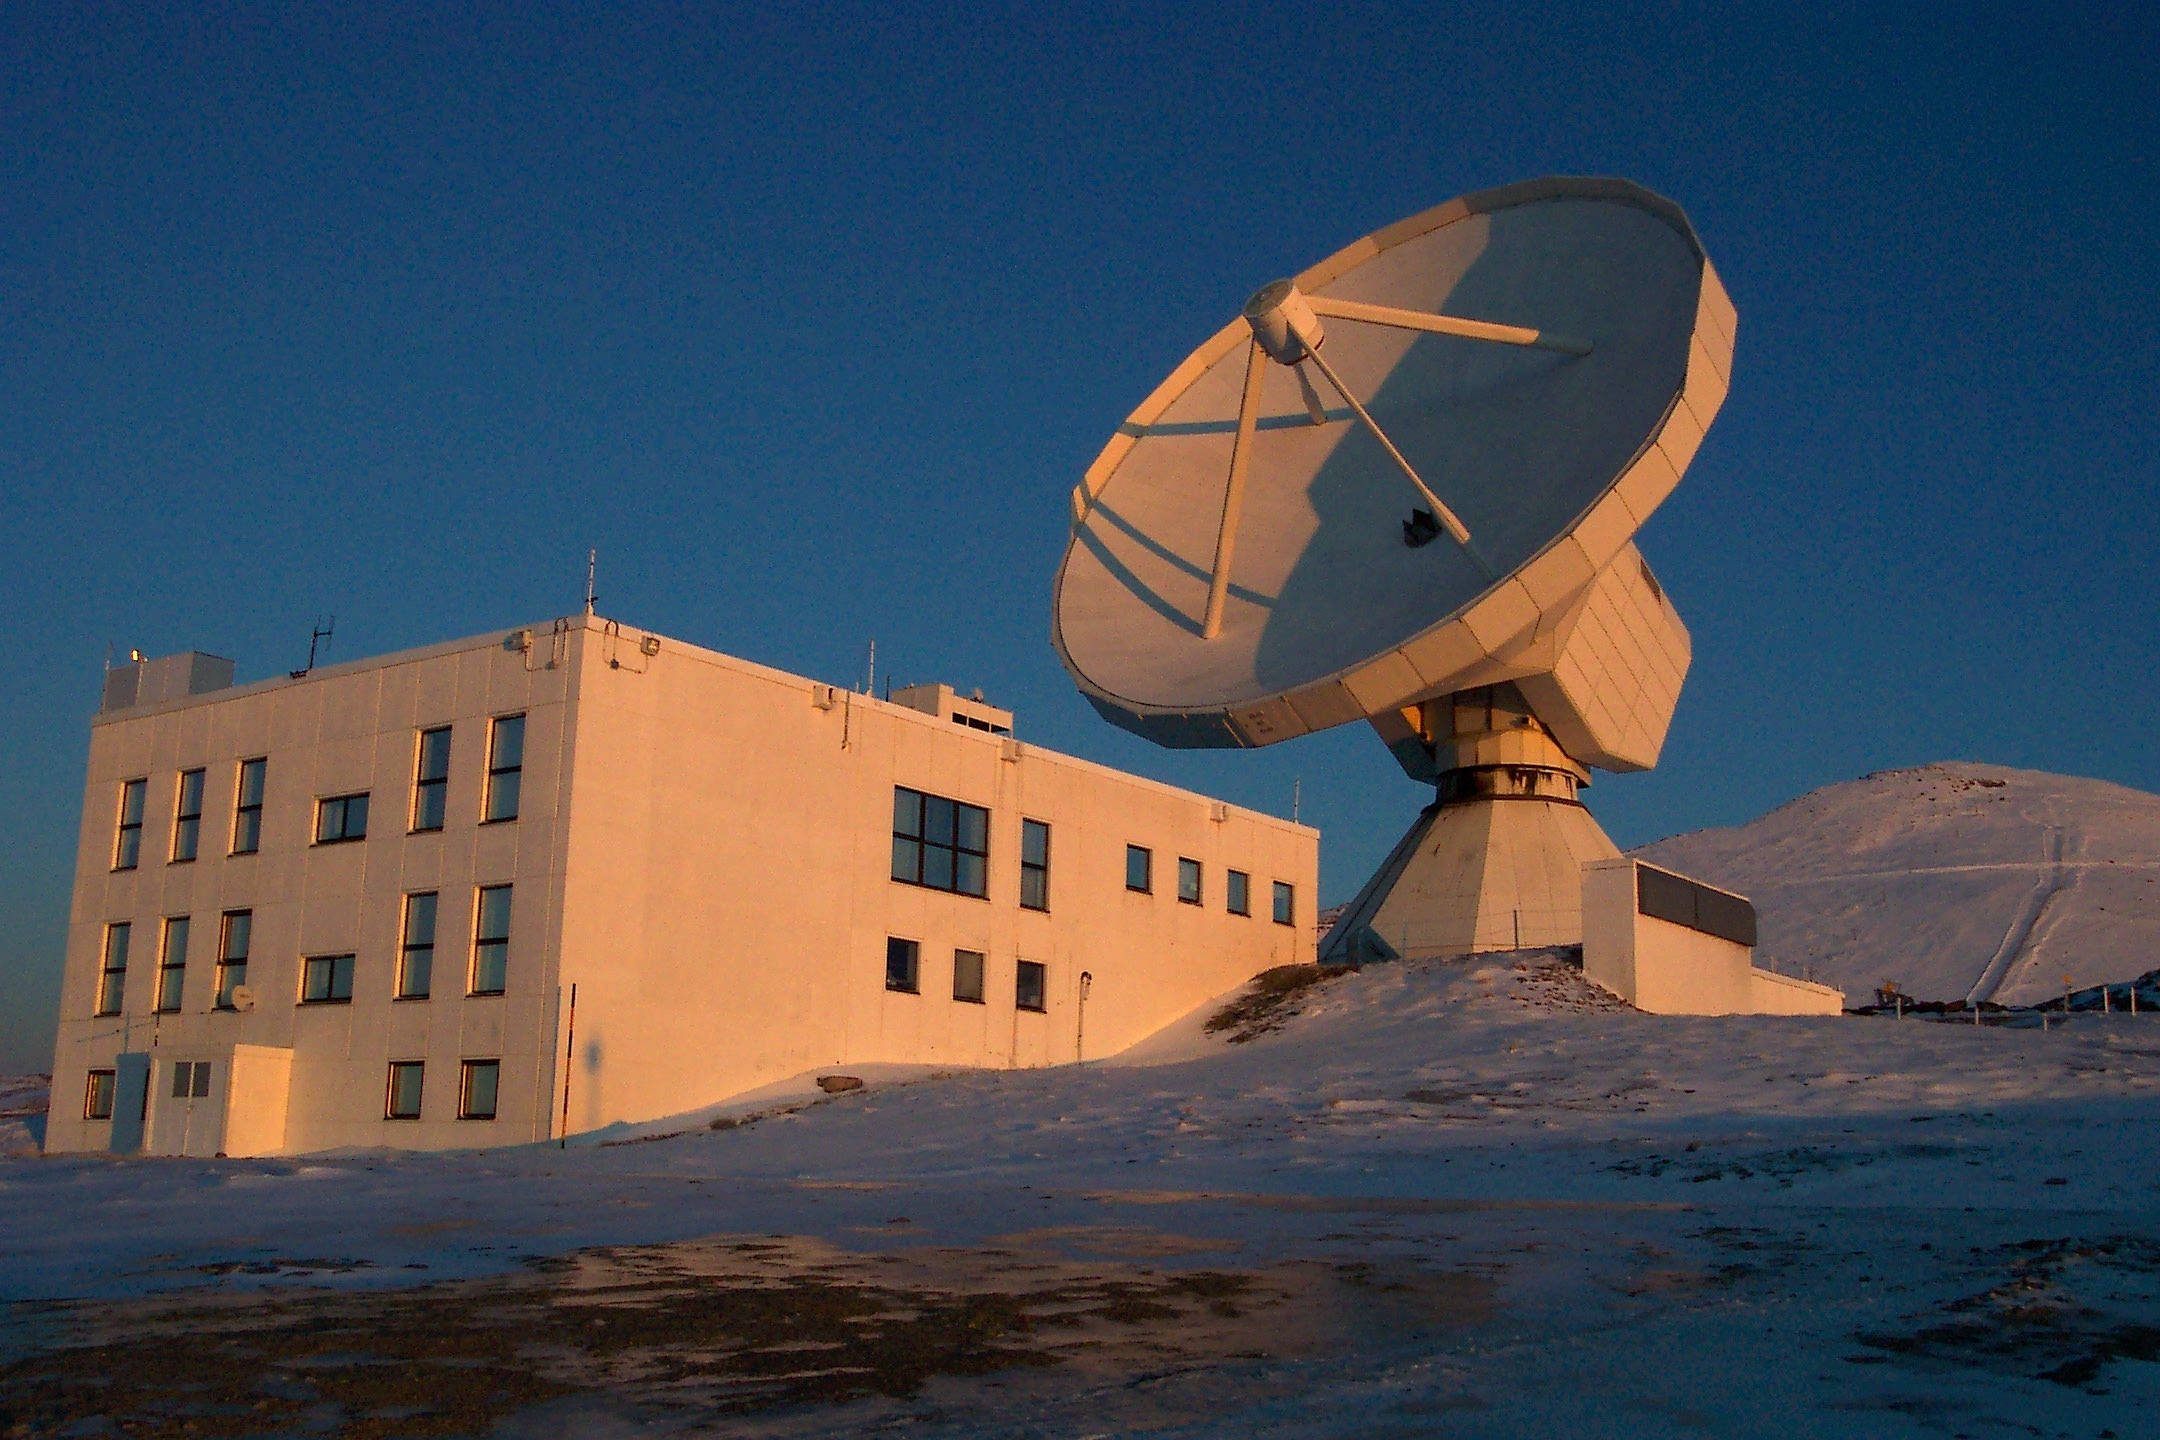
\includegraphics[width=\textwidth]
				{fig/IRAM_30m.jpg}
				\caption[IRAM 30-meter antenna.]
				{
					IRAM 30-meter antenna, next to the residential
					and control building, near Pico
					Veleta (visible on the right side of the
					picture), at Sierra Nevada, Granada. Picture by
					the author.
				}
		\label{fig:iram30m}
			\end{center}
		\end{figure}
		
		
		The IRAM~30m ---shown on figure~\ref{fig:iram30m} next
		to the residence and control building--- hosts several
		instruments, both coherent (heterodyne) and incoherent
		(bolometers), with different data reduction packages and
		techniques. There are also single-pixel and multi-pixel
		detectors, what makes the data handling even more
		particular.
		
		As the data from the detectors can be fed to several
		analysis systems, the former are called front-ends, while
		the latter are called back-ends. Keeping the different
		frontend-backend combinations is one of the complications
		of data storage for the IRAM~30m.
		
		And apart from the different frontend-backend combinations,
		one of the most complex parts of data handling for
		astronomical observatories is the handling of observing
		modes, compounded in radio astronomy with the combination
		of switching modes. They have been compiled, and briefly
		explained, in table~\ref{tabIRAM30mObservingSwitchingModes}.
		The definitive guide to the different observing modes,
		switching modes, front-ends, backends, and observing setup,
		is the guide to the IRAM New Control System (NCS) user
		interface\urlnote{\irampakourl}~\cite{2007pako.iram..109U}.
		
		\renewcommand{\tabularxcolumn}[1]{m{#1}}
		\begin{table}[tp]
		\begin{minipage}{\linewidth}
			\caption[Observing and switching modes of the IRAM~30m]
			{
				Available combinations of observing and switching
				modes at the IRAM~30m telescope. See notes
				and discussion on the text.
			}
			\label{tabIRAM30mObservingSwitchingModes}
		\begin{center}
		\begin{small}
		\begin{tabularx}{\linewidth}
			{>{\raggedleft\arraybackslash}m{3.25cm} cccc}
			
			\textbf{Observing mode} & 
			\textbf{swTotal}\footnote{In total power observations
			there is, in fact, no switching. See exception at psw
			switching.} &
			\textbf{swBeam}\footnote{In beam switching, the optical
			path is cut several times per observing cycle by the
			periodic interposition of a rotating blade (chopper).
			\invisiblenote{The
			off-source observation allows the estimation of the
			noise in the circuit.}} &
			\textbf{swWobbler}\footnote{In wobbler switching
			observations, the secondary mirror
			\invisiblenote{(the one monted
			on the quadrupod)} \emph{wobbles}, changing inclination
			slightly, effectively switching the beam to a different
			sky position.
			\invisiblenote{The off position changes during time
			around the source, due to the altazimuthal mount
			of the radio telescope.}} &
			\textbf{swFreq}\footnote{In frequency switching
			observations, the same position in the sky is observed
			at different frequencies.
			\invisiblenote{The emission of the source is
			expected to decrease at higher frequencies, while sky
			noise is maintained.}} \\ \midrule
		
			Calibrate (Heterodyne)\footnote{Calibrate observations
			are performed for heterodyne receivers in order to be
			able to convert from voltages/counts to fluxes.
			\invisiblenote
			{This is performed by observing the sky, a calibration
			load at ambient temperature, and a calibration load at
			about the temperature of liquid nitrogen.}} & 
			X & & & \\\addlinespace
			
			Pointing\footnote{Pointing observations are done to
			optimise the positioning of the telescope in Azimuth and
			Elevation.  This is done by continuum
			observations of a cross scan in azimuth and elevation on
			a point source \invisiblenote{(or at least a small
			source)} near the
			intended target source.
			\invisiblenote{The different switching modes
			correspond to different instrument setups, and should
			be the same as for the subsequent observations.}} &
			X &
			X &
			X & \\\addlinespace
		
			Focus\footnote{Focus observations are done to minimise
			the spread of received energy, maximising the collected
			energy. \invisiblenote{They are performed in the same
			switching mode
			as the Pointing and actual observations will be
			performed.}} &
			X &
			X &
			X & \\\addlinespace
		
			Tip (Skydip)\footnote{Tip, antenna tipping, or
			\emph{skydip} observations are performed in order to
			estimate the actual opacity of the atmosphere at
			different air masses (amount of atmosphere in the
			line of sight). \invisiblenote{This is more important for
			bolometer receivers, as heterodyne receivers can
			estimate opacity from their own observations.}} &
			X & & &
			\\\addlinespace
		
			Track\footnote{In Track or Tracking observations
			the position of the antenna does not change in celestial
			coordinates, and the off-source reference is taken by
			switching receiver frequency. \invisiblenote{This is
			particularly useful
			for estimating a line emission against continuum.
			if other line (astronomical or
			atmospherical) is present the observation is useless}} & 
			  &  &  & X \\\addlinespace
		
			On-Off\footnote{Observations made by comparison on
			the signal from a source and from a zero emission
			reference.} &
			psw\footnote{psw: Position switching, where the antenna
			drifts from the on to the off position. For total power
			observations, the complete power patter during the drift
			is also recorded.} & &
			X\invisible{wsw} & \\\addlinespace
		
			OTF Map (Heterodyne)\footnote{On-The-Fly observations
			record antenna signal across a drift in space along
			pre-determined paths. For heterodyne receivers, it
			creates data cubes.} & 
			X & & &
			X \\\addlinespace
		
			%Raster \\\addlinespace
		
			OTF Map (MAMBO Bolometer)\footnote{On-The-Fly
			observations with bolometers create intensity maps
			by recording intensities along pre-determined paths.} & & &
			X & \\\addlinespace
		
			VLBI\footnote{VLBI (Very Long Baseline Interferometry) 
			observations \invisiblenote{require special equipment,
			and} are not
			stored by the IRAM.\invisiblenote{instead are handled
			by the VLBI consortium.}} &
			X \\
		\end{tabularx}
		\end{small}
		\end{center}
		\end{minipage}
		\end{table}
		
		\subsection{Archive architecture} % (fold)
		\label{sub:archive_architecture_iram30}
			
			The architecture of the IRAM~30m archive is very similar
			to that of the DSS-63 archive, and follows the same
			principles of independence from the control system
			operation (in this case, the IRAM NCS), and of 
			layering of dependencies/responsibilities.
			Figure~\ref{figIramArchiveArchitecture} shows that
			architecture, and can be easily compared with
			figure~\ref{figDss63ArchiveArchitecture}
			
			\begin{figure}[tbp]
				\begin{center}
					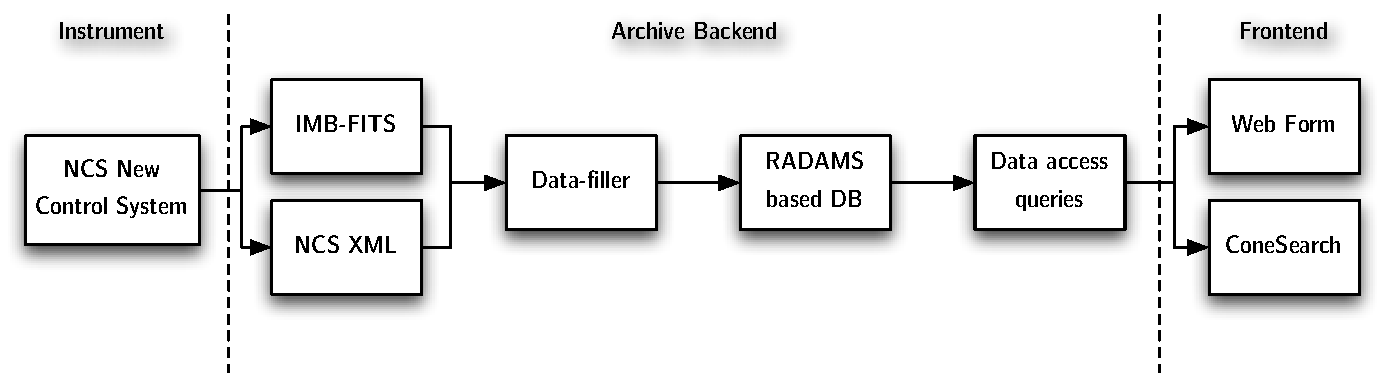
\includegraphics[width=\textwidth]
					{fig/IRAM30m_ArchiveArchitecture.pdf}
				\end{center}
				\caption[High level, layered architecture for the
				IRAM~30m archive]
				{High level, layered architecture of the 
				archive for the IRAM~30m antenna. Dotted lines
				represent the logical separation between layers.
				Arrows represent data flow between sub-systems.
				Communications between layers are confined to the
				communications established between interfacing
				components.}
				\label{figIramArchiveArchitecture}
			\end{figure}
			
			The differences in the workflow and working
			architecture between the DSS-63 and IRAM~30m are
			essentially related to the difference in the control
			system: whereas the JPL control system used by all
			DSS antennas provides FITS files in a format common
			to al DSCCs, and other JPL sites, together with
			text logs in the same format, the IRAM~30m uses since
			2005 the New Control System~\cite{2007pako.iram..109U,
			Brunswig:2002ul, Brunswig:2004gf, Hily-Blant:2001ve,
			Perrigouard:2005rz, Ungerechts:2002hl}, a Python-based
			real time telescope control system which writes each
			scan in a different IRAM Multi-Beam
			FITS~\cite{MudPolHat0512Multi-Beam} file, while at the
			same each observation is described in an XML
			file~\cite{Brunswig:2004gf}.
			
		% subsection archive_architecture_iram30 (end)
		
		\subsection{RADAMS implementation} % (fold)
		\label{sub:radams_implementation_iram}
			
			Given that the high-level architecture is
			largely the same for both archives, the differences
			between them have to deal with the different
			source data format (JPL FITS versus IMB-FITS), 
			observation logs (JPL text logs versus NCS XML files),
			and different database for supporting the additional
			observing modes, switching modes, and instruments
			available at the IRAM~30m.
			
			This additional complexity could be easily imagined by
			comparing table~\ref{tabIRAM30mObservingSwitchingModes}
			to the observation description for DSS-63 made in
			subsection~\ref{sub:spectral_observations_dss63}: the
			observing modes possible with DSS-63 are just those
			available for heterodyne receivers, and 
			wobbler-switching is not available.
			
			\begin{figure}[tbp]
				\centering
					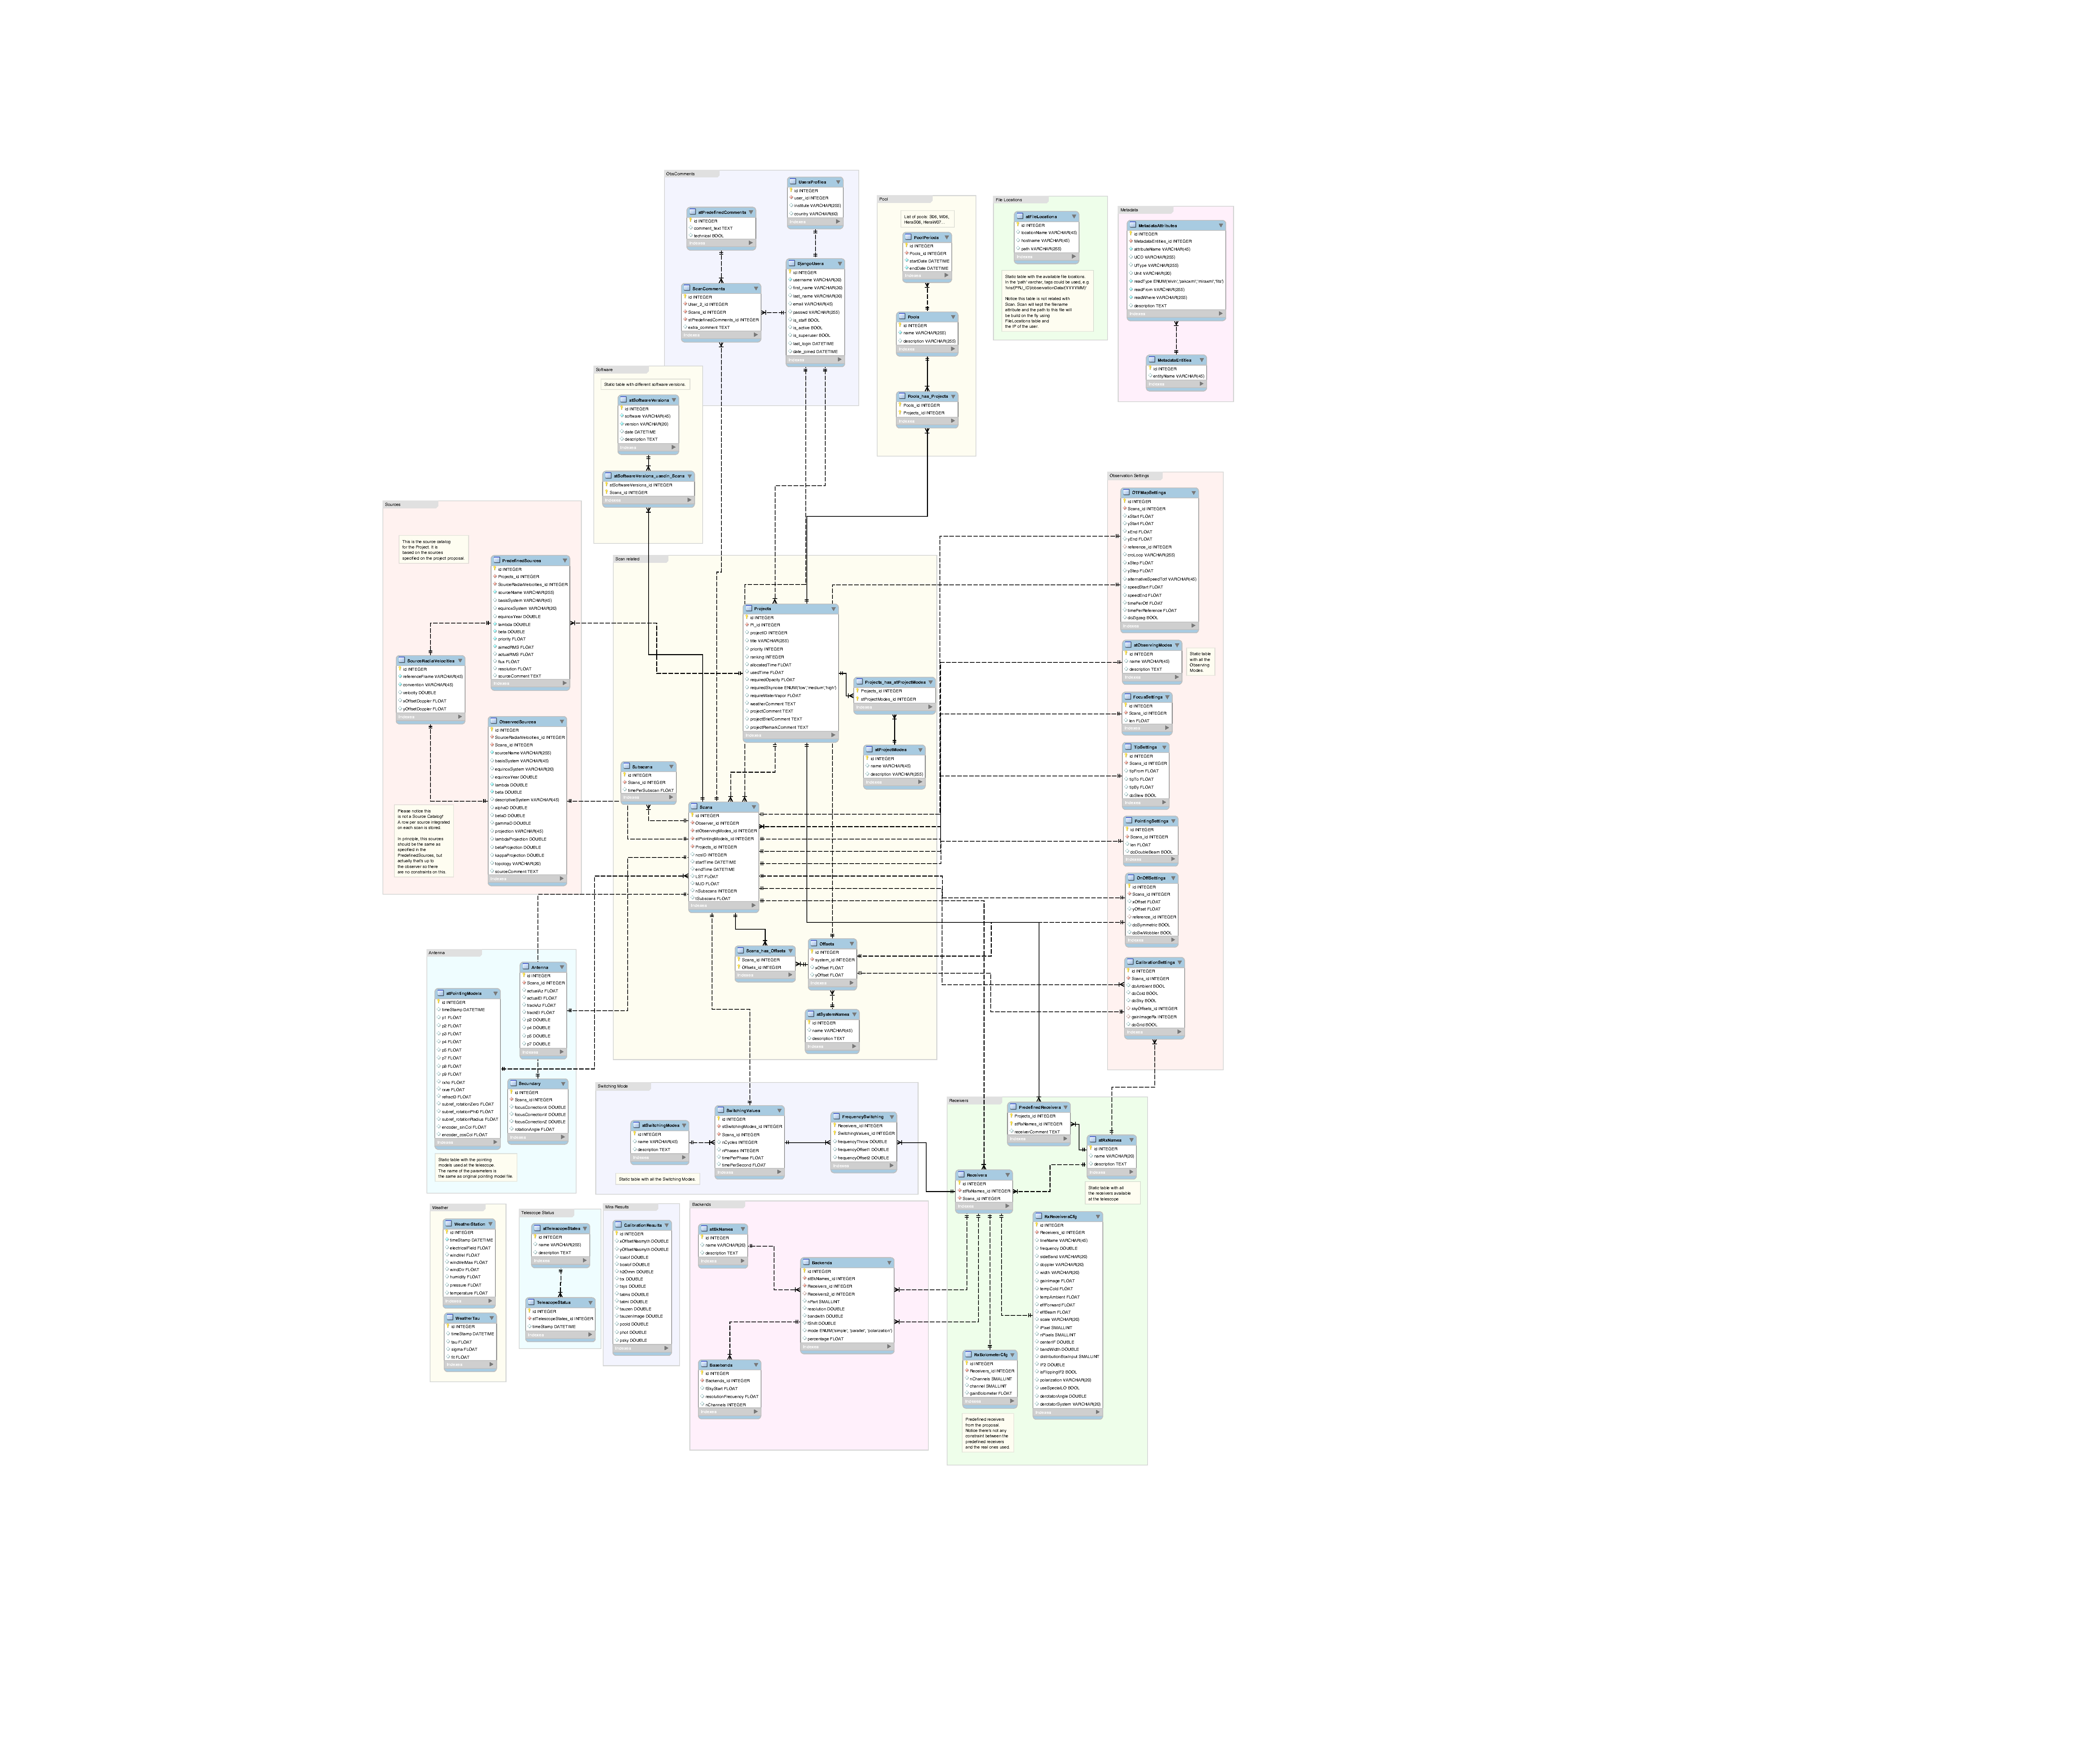
\includegraphics[totalheight=1.1\textheight]
					{fig/tapas-dm.pdf}
				\caption[Implementation of the data model for the
				IRAM~30m archive]
				{
					Implementation of the data model for the
					IRAM~30 archive, TAPAS (Telescope Archive
					for Public Access System). Generated by reverse
					engineering of the MySQL database.
				}
				\label{fig:fig_iram30m-data-model}
			\end{figure}
			
			Figure~\ref{fig:fig_iram30m-data-model} shows the
			database tables and relationships for the IRAM~30m
			database, named TAPAS (Telescope Archive for
			Public Access System). If we compare it with the DSS-63
			database in figure~\ref{fig:fig_DSS63-data-model}, we
			can see there are many more observing setting tables
			(each one holding different data for each different
			observing mode), and many more Project and Policy
			tables, in order to connect the archived data with the
			existing Pool database\footnote{The Pool database is a
			parallel system used to record project data for
			observing projects to be managed under \emph{pool}
			mode, that is, not having a fixed observing block, but
			instead allocating observing blocks following priority
			criteria for observable sources at any given time,
			using backup projects with less stringent weather
			conditions when high-priority projects cannot be
			observed.}.
			
			Given the higher complexity of the TAPAS database, we
			will perform a detailed comparison of RADAMS entities
			with the archive tables.
			
			\begin{description}
				\item[Observation] Observation is the root class for
				the data model, and serves to bind together all
				related information data and metadata. As such,
				it can be thought of as being embodied by the
				Scans table, with the caveats mentioned before
				about the extra number of dependencies.

				\item[ObsData] ObsData is a proxy to the actual
				observation data. In the case of TAPAS, these are
				raw and reduced IMB-FITS files. A separate table,
				stFileLocations, is used to contain the prefix
				path to where data will actually be located
				(accessible from the TAPAS system). As TAPAS file
				names are systematic\footnote{The file name is of
				the form
				\texttt{iram30-backend-yyyymmddsnn-imb.fits}, where
				backend represents the backend name (i.e.,
				\texttt{wilma}, \texttt{4mhz}, \texttt{vespa}...);
				\texttt{yyyymmdd} represents a date in
				year-month-day format; and \texttt{nn} is the scan
				number, separated from the date by an \texttt{s}.
				An example filename:
				\texttt{iram30m-vespa-20090211s62-imb.fits}}, they
				are built from Scan metadata and the
				stFileLocations table on the fly.

				\item[Target] Describes the target of the observation,
				providing as much information as available for
				already known targets, as discussed in
				section~\ref{subTargetDesc}.
				
				This part of RADAMS is supported in TAPAS by the
				tables ObservedSources and PredefinedSources
				tables.  PredefinedSources contains the sources
				which have been proposed for an observing project,
				and are linked to it\footnote{There is a CALIB 
				observation project in which usual flux, focus
				and pointing calibration sources are included.},
				while ObservedSources
				contains the sources which have actually been
				observed, with the target-related observation
				settings required. In the case of ObservedSources,
				coordinates are given in a generic spherical system
				which is converted into equatorial or other
				systems following the basisSystem and projection
				settings.
				
				Both tables are joined to a SourceRadialVelocities
				tables where recession velocities for well-known
				sources are stored, in order to properly set
				Velocity measurements.

				\item[Characterisation] This is the core of the
				RADAMS and generic observation models, and
				corresponds fully to the Characterisation data
				model Recommendation~\cite{2008dmadcrept.....L},
				as we have discussed in
				section~\ref{subObsDataCharacterisation}.
				
				We will describe separately the origin of
				Characterisation data for each of the axes:
				Spatial, Temporal, Spectral, and Observable.
				
				\begin{description}
					\item[Spatial] For most single-dish
					observations, Location, Bounds and Support
					are the same, and will be taken from the
					relationship between the Scans table and
					the PredefinedSources and ObservedSources
					tables. For OTF mapping, Location is
					taken from the PredefinedSources table,
					while Bounds will be calculated from
					projections of the \mapkey{xStart},
					\mapkey{yStart}, \mapkey{xEnd} and
					\mapkey{yEnd} derived from the ObservedSources
					metadata, while if Support is to be specified
					it has to be calculated from the \mapkey{xStep} 
					and \mapkey{yStep} attributes. For bolometer
					mapping, the Bounds and Support are the
					same\footnote{Support could be defined as a
					2D function on the RMS achieved across the map.},
					but they should be computed by the reduction
					software, or approximated by a convolution of
					observed coordinates  with beam widths.
					
					The coordinate computations for the observations
					have also to take into account the Offsets table,
					as those offsets can be added by the observer
					(following observing project instructions) to 
					use the same observing scripts to scan an offset
					part of the sky. See section 6.1 of the
					\emph{paKo user's
					guide}~\cite{2007pako.iram..109U} for a
					discussion of NCS-supported coordinate systems.
					
					Regarding spatial Resolution, this is a function
					of Antenna, Secondary, Observing mode, Receivers
					and Backends, and is looked up from engineering
					databases.
					
					For spatial accuracy, all data for pointing
					corrections is collected for all scans, and
					statistically studied by the engineering team.
					The Antenna table contains the intended and
					actual elevation and azimuth of the antenna,
					which allows for taking into account the
					average tracking system error, while parameters
					\mapkey{p1} to \mapkey{p9} of the IRAM pointing
					model~\cite{2000SPIE.4015..632P} are also stored,
					and can be used to optimise the pointing model.
					In particular, the observer adds the pointing
					corrections to the Antenna \mapkey{p2} ---azimuth
					correction--- and \mapkey{p7} ---elevation
					correction--- attributes.
					
					
					\item[Temporal] Location in the Temporal axis
					will be defined as the Scan \mapkey{startTime}
					attribute, with Bounds taken from
					\mapkey{startTime} and mapkey{endTime}. In order
					to provide Support the dead times between Scans
					should be calculated, but are not provided.
					
					\item[Spectral] The RADAMS defines the Location
					in the Spectral axis as the frequency for the
					central sample of the spectrum, which
					corresponds to the \mapkey{frequency} attribute
					of the ReceiversCfg table. Bounds are defined
					as that frequency, plus/minus half the
					\mapkey{bandwidth} attribute. Most of the metadata
					for the root AxisFrame.Spectral class is also
					recovered from the ReceiversCfg table.
					The Sensitivity will be compiled from the
					engineering measurements for the receiver, and
					will not be stored in TAPAS, while Resolution
					is compiled from the \mapkey{resolution}
					attribute in the Backends table.
					
					SamplingPrecision is also a function of the
					Backend, and will be stored and looked up from
					a static table.
					
					\item[Observable] For flux observations, such
					as On/Off observations, Location is taken
					from the \mapkey{flux} attribute of
					ObservedSource, while bounds is taken to be
					the interval at that value plus/minus the
					\mapkey{actualRMS} value. We do not provide
					Support for the Observable axis, while
					flux resolution is calculated as \mapkey{flux}
					divided by \mapkey{actualRMS}.
					
					As for flux accuracy, the values should be
					computed from statistics on historical data
					one the TAPAS database is in operation for at
					least a whole semester.
				\end{description}

				\item[Provenance] We will study the implementation
				of Provenance separately for each sub-model:
				
				\begin{description}
					\item[Provenance.Instrument] This part of
					Provenance was discussed in
					section~\ref{sec:instrumental_provenance}. It
					was defined as a hierarchical tree aggregating
					different subsystem configurations:
					Instrument\-Conf could hold several
					Antenna\-Conf entries (for describing
					antenna arrays), one or several Feeds per
					Antenna\-Conf, and one Bean\-Conf per
					Feed stating Beam properties, Receiver
					properties, Spectrum properties and
					Velocity properties.
					
					In TAPAS, the specific Instrument, Location
					and Instrument\-Conf classes are pre-computed
					and stored outside of the TAPAS database.
					The Antenna description part of the RADAMS
					needed to be updated for the IRAM~30m, and
					include the different switching modes, the
					configuration of the Secondary mirror (needed
					for wobbler switching modes). Beam metadata
					needs to be looked up in engineering
					configuration tables, and Receiver,
					Spectrum, and Velocity settings are obtained
					from the Receivers and Backends tables.
					
					
					\item[Provenance.AmbientConditions] This
					part of the RADAMS is directly linked to
					the WeatherStation and WeatherTau tables,
					using timestamps to correlate scans with
					measurements.
					
					In addition, the OpacityCurve is directly
					obtained from the results of observations
					of Tip kind\footnote{Scans with
					\mapkey{stObservingModes\_id} attribute
					corresponding to Tip or Bolotip observations.}.
					The CalibrationResults table holds that
					information for heterodyne receivers, reduced
					with the MIRA package.
					
					
					\item[Provenance.Processing] Some parts of
					Provenance.Processing are implemented on the
					TAPAS database, in particular the Software
					package-related metadata. The calibration
					part is still being reviewed, as different
					packages (MIRA, MOPSIC) provide very
					different processing and calibration
					information. 
					
					
				\end{description}

				\item[Curation] This part of the RADAMS is described
				in section~\ref{sec:curation}. The common curation
				data for TAPAS (the Curation table) is held outside
				of this database, and will be used for creating the
				ConeSearch entry in VO Registries. Project and
				DataID are obtained from the Scans and Project
				tables.
				
				There are plans to link the existing Proposal
				handling database to  the TAPAS system, and in that
				case the remaining Curation data model will be
				implemented.

				\item[Policy] As mentioned in
				section~\ref{sec:policy}, the Policy determination
				algorithm needs to get access to Users, Project,
				and observation related information such as
				Observers, Operators, et cetera.
				
				In TAPAS, Project information is stored in the
				Project table, with a link to the Principal
				Investigator, while Scan holds the Observer
				identifier, and Operators and Observatory staff have
				entries in the DjangoUsers table with the
				\mapkey{isStaff} set to true.
				
				The main difference with the proposed RADAMS
				architecture is that Operators are not identified
				with observations, and that there is no possibility
				to specify Co-Investigators.

				\item[Packaging] The TAPAS archive has all the
				infrastructure needed for being able to provide
				data in the form of VO services. However, due to the
				actual IRAM Policy statement, only header information
				will be publicly available for observations, after
				a 12 years proprietary period, while data themselves
				will only be available for a selection of projects,
				and only after 18 months proprietary period.
				The actual implementation of the Packaging class
				has not been, therefore, adapted to the TAPAS
				archive.
			\end{description}
			
			
			
			
			\newcommand{\iramthirtymetersqlurl}
		{http://www.iaa.es/~jdsant/thesis/iram30m-sourceDM-v0_8.sql}
			The complete SQL file implementing the IRAM~30m archive
			data base can be downloaded from the
			following link:\\
			\url{\iramthirtymetersqlurl}
			
			\suppress[Juande]
			{
			Listing~\ref{lst:iram30m-sql} shows the first SQL
			statements for the Django based archive.
			
			\lstinputlisting[
				language=SQL,
				caption={[SQL statements for IRAM~30m archive data
				model]
				First SQL statements for the IRAM~30m data model.
				
				},
				label=lst:iram30m-sql,
				firstline=1,
				lastline=65,
				float=tbp
			]
			{listing/iram30m-sourceDM-v0_8.sql}
			
			In order to be able to compare the RADAMS with the
			actual database for the IRAM~30m, the following pages
			are devoted to show all tables and attributes, with
			data types, ability to hold null files and default
			values.
			
			Table primary keys are in \textbf{\emph{bold italics}},
			while unique fields are in \textbf{bold}.
			
			\clearpage
			
			% phpMyAdmin LaTeX Dump
% version 2.11.7.1
% http://www.phpmyadmin.net
%
% Servidor: localhost
% Tiempo de generación: 25-03-2009 a las 22:22:56
% Versión del servidor: 5.0.41
% Versión de PHP: 5.2.6
% 
% Base de datos: 'IRAM30m'
% 

%
% Estructura: Antenna
%

\begin{longtable}{lcccl}
 
 \caption{Structure of table \texttt{Antenna}} \label{tab:Antenna-structure} \\
 \addlinespace \textbf{Field} & \textbf{Type} & \textbf{Null} & \textbf{Default}  \\ \midrule
\endfirsthead
 \caption*{Structure of table \texttt{Antenna} (continued)} \\ 
 \addlinespace \textbf{Field} & \textbf{Type} & \textbf{Null} & \textbf{Default}  \\ \midrule \endhead \endfoot
\textbf{\textit{id}} & int(11) & Yes & NULL \\ \addlinespace 
scan\_id & int(11) & Yes &  \\ \addlinespace 
actualAz & double & Yes & NULL \\ \addlinespace 
actualEl & double & Yes & NULL \\ \addlinespace 
trackAz & double & Yes & NULL \\ \addlinespace 
trackEl & double & Yes & NULL \\ \addlinespace 
p2 & double & Yes & NULL \\ \addlinespace 
p4 & double & Yes & NULL \\ \addlinespace 
p5 & double & Yes & NULL \\ \addlinespace 
p7 & double & Yes & NULL \\  
\end{longtable}

%
% Estructura: Backends
%
 \begin{longtable}{lcccl}
 
 \caption{Structure of table \texttt{Backends}} \label{tab:Backends-structure} \\
 \addlinespace \textbf{Field} & \textbf{Type} & \textbf{Null} & \textbf{Default}  \\ \midrule
\endfirsthead
 \caption*{Structure of table \texttt{Backends} (continued)} \\ 
 \addlinespace \textbf{Field} & \textbf{Type} & \textbf{Null} & \textbf{Default}  \\ \midrule \endhead \endfoot
\textbf{\textit{id}} & int(11) & Yes & NULL \\ \addlinespace 
bkName\_id & int(11) & Yes &  \\ \addlinespace 
receiver\_id & int(11) & Yes &  \\ \addlinespace 
receiver2\_id & int(11) & Yes & NULL \\ \addlinespace 
nPart & int(11) & Yes & NULL \\ \addlinespace 
resolution & double & Yes & NULL \\ \addlinespace 
bandwith & double & Yes & NULL \\ \addlinespace 
fShift & double & Yes & NULL \\ \addlinespace 
mode & varchar(36) & Yes &  \\ \addlinespace 
percentage & double & Yes & NULL \\  
 \end{longtable}

%
% Estructura: Basebands
%
 \begin{longtable}{lcccl}
 
 \caption{Structure of table \texttt{Basebands}} \label{tab:Basebands-structure} \\
 \addlinespace \textbf{Field} & \textbf{Type} & \textbf{Null} & \textbf{Default}  \\ \midrule
\endfirsthead
 \caption*{Structure of table \texttt{Basebands} (continued)} \\ 
 \addlinespace \textbf{Field} & \textbf{Type} & \textbf{Null} & \textbf{Default}  \\ \midrule \endhead \endfoot
\textbf{\textit{id}} & int(11) & Yes & NULL \\ \addlinespace 
backend\_id & int(11) & Yes &  \\ \addlinespace 
fSkyStart & double & Yes & NULL \\ \addlinespace 
resolutionFrecuency & double & Yes & NULL \\ \addlinespace 
nChannels & int(11) & Yes & NULL \\  
 \end{longtable}

%
% Estructura: CalibrationSettings
%
 \begin{longtable}{lcccl}
 
 \caption{Structure of table \texttt{CalibrationSettings}} \label{tab:CalibrationSettings-structure} \\
 \addlinespace \textbf{Field} & \textbf{Type} & \textbf{Null} & \textbf{Default}  \\ \midrule
\endfirsthead
 \caption*{Structure of table \texttt{CalibrationSettings} (continued)} \\ 
 \addlinespace \textbf{Field} & \textbf{Type} & \textbf{Null} & \textbf{Default}  \\ \midrule \endhead \endfoot
\textbf{\textit{id}} & int(11) & Yes & NULL \\ \addlinespace 
scan\_id & int(11) & Yes &  \\ \addlinespace 
doAmbient & tinyint(1) & Yes & NULL \\ \addlinespace 
doCold & tinyint(1) & Yes & NULL \\ \addlinespace 
doSky & tinyint(1) & Yes & NULL \\ \addlinespace 
skyOffset\_id & int(11) & Yes & NULL \\ \addlinespace 
gainimagerx & int(11) & Yes & NULL \\ \addlinespace 
doGrid & tinyint(1) & Yes & NULL \\  
 \end{longtable}

%
% Estructura: FocusSettings
%
 \begin{longtable}{lcccl}
 
 \caption{Structure of table \texttt{FocusSettings}} \label{tab:FocusSettings-structure} \\
 \addlinespace \textbf{Field} & \textbf{Type} & \textbf{Null} & \textbf{Default}  \\ \midrule
\endfirsthead
 \caption*{Structure of table \texttt{FocusSettings} (continued)} \\ 
 \addlinespace \textbf{Field} & \textbf{Type} & \textbf{Null} & \textbf{Default}  \\ \midrule \endhead \endfoot
\textbf{\textit{id}} & int(11) & Yes & NULL \\ \addlinespace 
scan\_id & int(11) & Yes &  \\ \addlinespace 
len & double & Yes & NULL \\  
 \end{longtable}

%
% Estructura: FrequencySwitching
%
 \begin{longtable}{lcccl}
 
 \caption{Structure of table \texttt{FrequencySwitching}} \label{tab:FrequencySwitching-structure} \\
 \addlinespace \textbf{Field} & \textbf{Type} & \textbf{Null} & \textbf{Default}  \\ \midrule
\endfirsthead
 \caption*{Structure of table \texttt{FrequencySwitching} (continued)} \\ 
 \addlinespace \textbf{Field} & \textbf{Type} & \textbf{Null} & \textbf{Default}  \\ \midrule \endhead \endfoot
\textbf{\textit{id}} & int(11) & Yes & NULL \\ \addlinespace 
receiver\_id & int(11) & Yes &  \\ \addlinespace 
switchingCfg\_id & int(11) & Yes &  \\ \addlinespace 
frequencyThrow & double & Yes & NULL \\ \addlinespace 
frequencyOffset1 & double & Yes & NULL \\ \addlinespace 
frequencyOffset2 & double & Yes & NULL \\  
 \end{longtable}

%
% Estructura: MetadataAttributes
%
 \begin{longtable}{lcccl}
 
 \caption{Structure of table \texttt{MetadataAttributes}} \label{tab:MetadataAttributes-structure} \\
 \addlinespace \textbf{Field} & \textbf{Type} & \textbf{Null} & \textbf{Default}  \\ \midrule
\endfirsthead
 \caption*{Structure of table \texttt{MetadataAttributes} (continued)} \\ 
 \addlinespace \textbf{Field} & \textbf{Type} & \textbf{Null} & \textbf{Default}  \\ \midrule \endhead \endfoot
\textbf{\textit{id}} & int(11) & Yes & NULL \\ \addlinespace 
metadataEntity\_id & int(11) & Yes &  \\ \addlinespace 
attributeName & varchar(45) & Yes &  \\ \addlinespace 
UCD & varchar(255) & Yes &  \\ \addlinespace 
UType & varchar(255) & Yes &  \\ \addlinespace 
unit & varchar(20) & Yes &  \\ \addlinespace 
readType & varchar(21) & Yes &  \\ \addlinespace 
readFrom & varchar(255) & Yes &  \\ \addlinespace 
readWhere & varchar(255) & Yes &  \\ \addlinespace 
description & longtext & Yes &  \\  
 \end{longtable}

%
% Estructura: MetadataEntities
%
 \begin{longtable}{lcccl}
 
 \caption{Structure of table \texttt{MetadataEntities}} \label{tab:MetadataEntities-structure} \\
 \addlinespace \textbf{Field} & \textbf{Type} & \textbf{Null} & \textbf{Default}  \\ \midrule
\endfirsthead
 \caption*{Structure of table \texttt{MetadataEntities} (continued)} \\ 
 \addlinespace \textbf{Field} & \textbf{Type} & \textbf{Null} & \textbf{Default}  \\ \midrule \endhead \endfoot
\textbf{\textit{id}} & int(11) & Yes & NULL \\ \addlinespace 
name & varchar(45) & Yes &  \\  
 \end{longtable}

%
% Estructura: ObservedSources
%
 \begin{longtable}{lcccl}
 
 \caption{Structure of table \texttt{ObservedSources}} \label{tab:ObservedSources-structure} \\
 \addlinespace \textbf{Field} & \textbf{Type} & \textbf{Null} & \textbf{Default}  \\ \midrule
\endfirsthead
 \caption*{Structure of table \texttt{ObservedSources} (continued)} \\ 
 \addlinespace \textbf{Field} & \textbf{Type} & \textbf{Null} & \textbf{Default}  \\ \midrule \endhead \endfoot
\textbf{\textit{id}} & int(11) & Yes & NULL \\ \addlinespace 
sourceRadialVelocity\_id & int(11) & Yes &  \\ \addlinespace 
scan\_id & int(11) & Yes &  \\ \addlinespace 
sourceName & varchar(255) & Yes &  \\ \addlinespace 
basisSystem & varchar(45) & Yes &  \\ \addlinespace 
equinoxSystem & varchar(20) & Yes &  \\ \addlinespace 
equinoxYear & double & Yes & NULL \\ \addlinespace 
lambda & double & Yes &  \\ \addlinespace 
beta & double & Yes &  \\ \addlinespace 
descriptiveSystem & varchar(45) & Yes &  \\ \addlinespace 
alphaD & double & Yes & NULL \\ \addlinespace 
betaD & double & Yes & NULL \\ \addlinespace 
gammaD & double & Yes & NULL \\ \addlinespace 
projection & varchar(45) & Yes &  \\ \addlinespace 
lambdaProjection & double & Yes & NULL \\ \addlinespace 
betaProjection & double & Yes & NULL \\ \addlinespace 
kappaProjection & double & Yes & NULL \\ \addlinespace 
topology & varchar(20) & Yes &  \\  
 \end{longtable}

%
% Estructura: Offsets
%
 \begin{longtable}{lcccl}
 
 \caption{Structure of table \texttt{Offsets}} \label{tab:Offsets-structure} \\
 \addlinespace \textbf{Field} & \textbf{Type} & \textbf{Null} & \textbf{Default}  \\ \midrule
\endfirsthead
 \caption*{Structure of table \texttt{Offsets} (continued)} \\ 
 \addlinespace \textbf{Field} & \textbf{Type} & \textbf{Null} & \textbf{Default}  \\ \midrule \endhead \endfoot
\textbf{\textit{id}} & int(11) & Yes & NULL \\ \addlinespace 
system\_id & int(11) & Yes &  \\ \addlinespace 
xOffset & double & Yes & NULL \\ \addlinespace 
yOffset & double & Yes & NULL \\  
 \end{longtable}

%
% Estructura: OnOffSettings
%
 \begin{longtable}{lcccl}
 
 \caption{Structure of table \texttt{OnOffSettings}} \label{tab:OnOffSettings-structure} \\
 \addlinespace \textbf{Field} & \textbf{Type} & \textbf{Null} & \textbf{Default}  \\ \midrule
\endfirsthead
 \caption*{Structure of table \texttt{OnOffSettings} (continued)} \\ 
 \addlinespace \textbf{Field} & \textbf{Type} & \textbf{Null} & \textbf{Default}  \\ \midrule \endhead \endfoot
\textbf{\textit{id}} & int(11) & Yes & NULL \\ \addlinespace 
scan\_id & int(11) & Yes &  \\ \addlinespace 
xOffset & double & Yes & NULL \\ \addlinespace 
yOffset & double & Yes & NULL \\ \addlinespace 
reference\_id & int(11) & Yes & NULL \\ \addlinespace 
doSymmetric & tinyint(1) & Yes & NULL \\ \addlinespace 
doSwWobbler & tinyint(1) & Yes & NULL \\  
 \end{longtable}

%
% Estructura: OTFMapSettings
%
 \begin{longtable}{lcccl}
 
 \caption{Structure of table \texttt{OTFMapSettings}} \label{tab:OTFMapSettings-structure} \\
 \addlinespace \textbf{Field} & \textbf{Type} & \textbf{Null} & \textbf{Default}  \\ \midrule
\endfirsthead
 \caption*{Structure of table \texttt{OTFMapSettings} (continued)} \\ 
 \addlinespace \textbf{Field} & \textbf{Type} & \textbf{Null} & \textbf{Default}  \\ \midrule \endhead \endfoot
\textbf{\textit{id}} & int(11) & Yes & NULL \\ \addlinespace 
scan\_id & int(11) & Yes &  \\ \addlinespace 
xStart & double & Yes & NULL \\ \addlinespace 
yStart & double & Yes & NULL \\ \addlinespace 
xEnd & double & Yes & NULL \\ \addlinespace 
yEnd & double & Yes & NULL \\ \addlinespace 
reference\_id & int(11) & Yes & NULL \\ \addlinespace 
croLoop & varchar(255) & Yes &  \\ \addlinespace 
xStep & double & Yes & NULL \\ \addlinespace 
yStep & double & Yes & NULL \\ \addlinespace 
alternativeSpeedTotf & varchar(45) & Yes &  \\ \addlinespace 
speedStart & double & Yes & NULL \\ \addlinespace 
speedEnd & double & Yes & NULL \\ \addlinespace 
timePerOtf & double & Yes & NULL \\ \addlinespace 
timePerReference & double & Yes & NULL \\ \addlinespace 
doZigzag & tinyint(1) & Yes & NULL \\  
 \end{longtable}

%
% Estructura: PointingSettings
%
 \begin{longtable}{lcccl}
 
 \caption{Structure of table \texttt{PointingSettings}} \label{tab:PointingSettings-structure} \\
 \addlinespace \textbf{Field} & \textbf{Type} & \textbf{Null} & \textbf{Default}  \\ \midrule
\endfirsthead
 \caption*{Structure of table \texttt{PointingSettings} (continued)} \\ 
 \addlinespace \textbf{Field} & \textbf{Type} & \textbf{Null} & \textbf{Default}  \\ \midrule \endhead \endfoot
\textbf{\textit{id}} & int(11) & Yes & NULL \\ \addlinespace 
scan\_id & int(11) & Yes &  \\ \addlinespace 
len & double & Yes & NULL \\ \addlinespace 
doDoubleBeam & tinyint(1) & Yes & NULL \\  
 \end{longtable}

%
% Estructura: Pools
%
 \begin{longtable}{lcccl}
 
 \caption{Structure of table \texttt{Pools}} \label{tab:Pools-structure} \\
 \addlinespace \textbf{Field} & \textbf{Type} & \textbf{Null} & \textbf{Default}  \\ \midrule
\endfirsthead
 \caption*{Structure of table \texttt{Pools} (continued)} \\ 
 \addlinespace \textbf{Field} & \textbf{Type} & \textbf{Null} & \textbf{Default}  \\ \midrule \endhead \endfoot
\textbf{\textit{id}} & int(11) & Yes & NULL \\ \addlinespace 
name & varchar(255) & Yes &  \\ \addlinespace 
description & varchar(255) & Yes &  \\  
 \end{longtable}

%
% Estructura: Pools_has_Projects
%
 \begin{longtable}{lcccl}
 
 \caption{Structure of table \texttt{Pools\_has\_Projects}} \label{tab:Pools_has_Projects-structure} \\
 \addlinespace \textbf{Field} & \textbf{Type} & \textbf{Null} & \textbf{Default}  \\ \midrule
\endfirsthead
 \caption*{Structure of table \texttt{Pools\_has\_Projects} (continued)} \\ 
 \addlinespace \textbf{Field} & \textbf{Type} & \textbf{Null} & \textbf{Default}  \\ \midrule \endhead \endfoot
\textbf{\textit{id}} & int(11) & Yes & NULL \\ \addlinespace 
\textbf{pools\_id} & int(11) & Yes &  \\ \addlinespace 
\textbf{project\_id} & int(11) & Yes &  \\  
 \end{longtable}

%
% Estructura: PredefinedReceivers
%
 \begin{longtable}{lcccl}
 
 \caption{Structure of table \texttt{PredefinedReceivers}} \label{tab:PredefinedReceivers-structure} \\
 \addlinespace \textbf{Field} & \textbf{Type} & \textbf{Null} & \textbf{Default}  \\ \midrule
\endfirsthead
 \caption*{Structure of table \texttt{PredefinedReceivers} (continued)} \\ 
 \addlinespace \textbf{Field} & \textbf{Type} & \textbf{Null} & \textbf{Default}  \\ \midrule \endhead \endfoot
\textbf{\textit{id}} & int(11) & Yes & NULL \\ \addlinespace 
project\_id & int(11) & Yes &  \\ \addlinespace 
rxName\_id & int(11) & Yes &  \\ \addlinespace 
commentReceiver & longtext & Yes &  \\  
 \end{longtable}

%
% Estructura: PredefinedSources
%
 \begin{longtable}{lcccl}
 
 \caption{Structure of table \texttt{PredefinedSources}} \label{tab:PredefinedSources-structure} \\
 \addlinespace \textbf{Field} & \textbf{Type} & \textbf{Null} & \textbf{Default}  \\ \midrule
\endfirsthead
 \caption*{Structure of table \texttt{PredefinedSources} (continued)} \\ 
 \addlinespace \textbf{Field} & \textbf{Type} & \textbf{Null} & \textbf{Default}  \\ \midrule \endhead \endfoot
\textbf{\textit{id}} & int(11) & Yes & NULL \\ \addlinespace 
project\_id & int(11) & Yes &  \\ \addlinespace 
sourceRadialVelocity\_id & int(11) & Yes &  \\ \addlinespace 
sourceName & varchar(255) & Yes &  \\ \addlinespace 
basisSystem & varchar(45) & Yes &  \\ \addlinespace 
equinoxSystem & varchar(20) & Yes &  \\ \addlinespace 
equinoxYear & double & Yes & NULL \\ \addlinespace 
lambda & double & Yes &  \\ \addlinespace 
beta & double & Yes &  \\ \addlinespace 
priority & double & Yes &  \\ \addlinespace 
aimedRMS & double & Yes &  \\ \addlinespace 
actualRMS & double & Yes & NULL \\ \addlinespace 
flux & double & Yes & NULL \\ \addlinespace 
comment & longtext & Yes &  \\  
 \end{longtable}

%
% Estructura: Projects
%
 \begin{longtable}{lcccl}
 
 \caption{Structure of table \texttt{Projects}} \label{tab:Projects-structure} \\
 \addlinespace \textbf{Field} & \textbf{Type} & \textbf{Null} & \textbf{Default}  \\ \midrule
\endfirsthead
 \caption*{Structure of table \texttt{Projects} (continued)} \\ 
 \addlinespace \textbf{Field} & \textbf{Type} & \textbf{Null} & \textbf{Default}  \\ \midrule \endhead \endfoot
\textbf{\textit{id}} & int(11) & Yes & NULL \\ \addlinespace 
observer\_id & int(11) & Yes &  \\ \addlinespace 
pi\_id & int(11) & Yes &  \\ \addlinespace 
projectId & int(11) & Yes & NULL \\ \addlinespace 
title & varchar(255) & Yes &  \\ \addlinespace 
priority & int(11) & Yes & NULL \\ \addlinespace 
ranking & int(11) & Yes & NULL \\ \addlinespace 
allocatedTime & double & Yes & NULL \\ \addlinespace 
usedTime & double & Yes & NULL \\ \addlinespace 
comment & longtext & Yes &  \\ \addlinespace 
requiredOpacity & double & Yes & NULL \\ \addlinespace 
requiredSkynoise & varchar(18) & Yes &  \\ \addlinespace 
weatherComment & longtext & Yes &  \\  
 \end{longtable}

%
% Estructura: Projects_has_stProjectModes
%
 \begin{longtable}{lcccl}
 
 \caption{Structure of table \texttt{Projects\_has\_stProjectModes}} \label{tab:Projects_has_stProjectModes-structure} \\
 \addlinespace \textbf{Field} & \textbf{Type} & \textbf{Null} & \textbf{Default}  \\ \midrule
\endfirsthead
 \caption*{Structure of table \texttt{Projects\_has\_stProjectModes} (continued)} \\ 
 \addlinespace \textbf{Field} & \textbf{Type} & \textbf{Null} & \textbf{Default}  \\ \midrule \endhead \endfoot
\textbf{\textit{id}} & int(11) & Yes & NULL \\ \addlinespace 
\textbf{project\_id} & int(11) & Yes &  \\ \addlinespace 
\textbf{stprojectmodes\_id} & int(11) & Yes &  \\  
 \end{longtable}

%
% Estructura: Receivers
%
 \begin{longtable}{lcccl}
 
 \caption{Structure of table \texttt{Receivers}} \label{tab:Receivers-structure} \\
 \addlinespace \textbf{Field} & \textbf{Type} & \textbf{Null} & \textbf{Default}  \\ \midrule
\endfirsthead
 \caption*{Structure of table \texttt{Receivers} (continued)} \\ 
 \addlinespace \textbf{Field} & \textbf{Type} & \textbf{Null} & \textbf{Default}  \\ \midrule \endhead \endfoot
\textbf{\textit{id}} & int(11) & Yes & NULL \\ \addlinespace 
rxName\_id & int(11) & Yes &  \\ \addlinespace 
scan\_id & int(11) & Yes &  \\  
 \end{longtable}

%
% Estructura: RxBolometerCfg
%
 \begin{longtable}{lcccl}
 
 \caption{Structure of table \texttt{RxBolometerCfg}} \label{tab:RxBolometerCfg-structure} \\
 \addlinespace \textbf{Field} & \textbf{Type} & \textbf{Null} & \textbf{Default}  \\ \midrule
\endfirsthead
 \caption*{Structure of table \texttt{RxBolometerCfg} (continued)} \\ 
 \addlinespace \textbf{Field} & \textbf{Type} & \textbf{Null} & \textbf{Default}  \\ \midrule \endhead \endfoot
\textbf{\textit{id}} & int(11) & Yes & NULL \\ \addlinespace 
receiver\_id & int(11) & Yes &  \\ \addlinespace 
nChannels & int(11) & Yes & NULL \\ \addlinespace 
channel & int(11) & Yes & NULL \\ \addlinespace 
gainBolometer & double & Yes & NULL \\  
 \end{longtable}

%
% Estructura: RxReceiversCfg
%
 \begin{longtable}{lcccl}
 
 \caption{Structure of table \texttt{RxReceiversCfg}} \label{tab:RxReceiversCfg-structure} \\
 \addlinespace \textbf{Field} & \textbf{Type} & \textbf{Null} & \textbf{Default}  \\ \midrule
\endfirsthead
 \caption*{Structure of table \texttt{RxReceiversCfg} (continued)} \\ 
 \addlinespace \textbf{Field} & \textbf{Type} & \textbf{Null} & \textbf{Default}  \\ \midrule \endhead \endfoot
\textbf{\textit{id}} & int(11) & Yes & NULL \\ \addlinespace 
receiver\_id & int(11) & Yes &  \\ \addlinespace 
lineName & varchar(45) & Yes &  \\ \addlinespace 
frequency & double & Yes & NULL \\ \addlinespace 
sideBand & varchar(20) & Yes &  \\ \addlinespace 
doppler & varchar(20) & Yes &  \\ \addlinespace 
width & varchar(20) & Yes &  \\ \addlinespace 
gainImage & double & Yes & NULL \\ \addlinespace 
tempCold & double & Yes & NULL \\ \addlinespace 
tempAmbient & double & Yes & NULL \\ \addlinespace 
effForward & double & Yes & NULL \\ \addlinespace 
effBeam & double & Yes & NULL \\ \addlinespace 
scale & varchar(20) & Yes &  \\ \addlinespace 
iPixel & int(11) & Yes & NULL \\ \addlinespace 
nPixels & int(11) & Yes & NULL \\ \addlinespace 
centerIF & double & Yes & NULL \\ \addlinespace 
bandwidth & double & Yes & NULL \\ \addlinespace 
distributionBoxInput & int(11) & Yes & NULL \\ \addlinespace 
IF2 & double & Yes & NULL \\ \addlinespace 
isFlippingIF2 & tinyint(1) & Yes & NULL \\ \addlinespace 
polarization & varchar(20) & Yes &  \\ \addlinespace 
useSpecialLO & tinyint(1) & Yes & NULL \\ \addlinespace 
derotatorAngle & double & Yes & NULL \\ \addlinespace 
derotatorSystem & varchar(20) & Yes &  \\  
 \end{longtable}

%
% Estructura: ScanComments
%
 \begin{longtable}{lcccl}
 
 \caption{Structure of table \texttt{ScanComments}} \label{tab:ScanComments-structure} \\
 \addlinespace \textbf{Field} & \textbf{Type} & \textbf{Null} & \textbf{Default}  \\ \midrule
\endfirsthead
 \caption*{Structure of table \texttt{ScanComments} (continued)} \\ 
 \addlinespace \textbf{Field} & \textbf{Type} & \textbf{Null} & \textbf{Default}  \\ \midrule \endhead \endfoot
\textbf{\textit{id}} & int(11) & Yes & NULL \\ \addlinespace 
scan\_id & int(11) & Yes &  \\ \addlinespace 
predefinedComment\_id & int(11) & Yes &  \\ \addlinespace 
User\_id & int(11) & Yes &  \\ \addlinespace 
extraComment & longtext & Yes &  \\  
 \end{longtable}

%
% Estructura: Scans
%
 \begin{longtable}{lcccl}
 
 \caption{Structure of table \texttt{Scans}} \label{tab:Scans-structure} \\
 \addlinespace \textbf{Field} & \textbf{Type} & \textbf{Null} & \textbf{Default}  \\ \midrule
\endfirsthead
 \caption*{Structure of table \texttt{Scans} (continued)} \\ 
 \addlinespace \textbf{Field} & \textbf{Type} & \textbf{Null} & \textbf{Default}  \\ \midrule \endhead \endfoot
\textbf{\textit{id}} & int(11) & Yes & NULL \\ \addlinespace 
system\_id & int(11) & Yes & NULL \\ \addlinespace 
observingMode\_id & int(11) & Yes &  \\ \addlinespace 
pointingModel\_id & int(11) & Yes &  \\ \addlinespace 
project\_id & int(11) & Yes &  \\ \addlinespace 
ncsId & int(11) & Yes & NULL \\ \addlinespace 
startTime & datetime & Yes & NULL \\ \addlinespace 
endTime & datetime & Yes & NULL \\ \addlinespace 
LST & double & Yes & NULL \\ \addlinespace 
MJD & double & Yes & NULL \\ \addlinespace 
nSubscans & int(11) & Yes & NULL \\ \addlinespace 
tSubscans & double & Yes & NULL \\  
 \end{longtable}

%
% Estructura: Scans_has_Offsets
%
 \begin{longtable}{lcccl}
 
 \caption{Structure of table \texttt{Scans\_has\_Offsets}} \label{tab:Scans_has_Offsets-structure} \\
 \addlinespace \textbf{Field} & \textbf{Type} & \textbf{Null} & \textbf{Default}  \\ \midrule
\endfirsthead
 \caption*{Structure of table \texttt{Scans\_has\_Offsets} (continued)} \\ 
 \addlinespace \textbf{Field} & \textbf{Type} & \textbf{Null} & \textbf{Default}  \\ \midrule \endhead \endfoot
\textbf{\textit{id}} & int(11) & Yes & NULL \\ \addlinespace 
\textbf{scan\_id} & int(11) & Yes &  \\ \addlinespace 
\textbf{offset\_id} & int(11) & Yes &  \\  
 \end{longtable}

%
% Estructura: Secondary
%
 \begin{longtable}{lcccl}
 
 \caption{Structure of table \texttt{Secondary}} \label{tab:Secondary-structure} \\
 \addlinespace \textbf{Field} & \textbf{Type} & \textbf{Null} & \textbf{Default}  \\ \midrule
\endfirsthead
 \caption*{Structure of table \texttt{Secondary} (continued)} \\ 
 \addlinespace \textbf{Field} & \textbf{Type} & \textbf{Null} & \textbf{Default}  \\ \midrule \endhead \endfoot
\textbf{\textit{id}} & int(11) & Yes & NULL \\ \addlinespace 
scan\_id & int(11) & Yes &  \\ \addlinespace 
focusCorrectionX & double & Yes & NULL \\ \addlinespace 
focusCorrectionY & double & Yes & NULL \\ \addlinespace 
focusCorrectionZ & double & Yes & NULL \\ \addlinespace 
rotationAngle & double & Yes & NULL \\  
 \end{longtable}

%
% Estructura: SourceRadialVelocities
%
 \begin{longtable}{lcccl}
 
 \caption{Structure of table \texttt{SourceRadialVelocities}} \label{tab:SourceRadialVelocities-structure} \\
 \addlinespace \textbf{Field} & \textbf{Type} & \textbf{Null} & \textbf{Default}  \\ \midrule
\endfirsthead
 \caption*{Structure of table \texttt{SourceRadialVelocities} (continued)} \\ 
 \addlinespace \textbf{Field} & \textbf{Type} & \textbf{Null} & \textbf{Default}  \\ \midrule \endhead \endfoot
\textbf{\textit{id}} & int(11) & Yes & NULL \\ \addlinespace 
referenceFrame & varchar(45) & Yes &  \\ \addlinespace 
convention & varchar(45) & Yes &  \\ \addlinespace 
velocity & double & Yes & NULL \\ \addlinespace 
xOffsetDoppler & double & Yes & NULL \\ \addlinespace 
yOffsetDoppler & double & Yes & NULL \\  
 \end{longtable}

%
% Estructura: stBkNames
%
 \begin{longtable}{lcccl}
 
 \caption{Structure of table \texttt{stBkNames}} \label{tab:stBkNames-structure} \\
 \addlinespace \textbf{Field} & \textbf{Type} & \textbf{Null} & \textbf{Default}  \\ \midrule
\endfirsthead
 \caption*{Structure of table \texttt{stBkNames} (continued)} \\ 
 \addlinespace \textbf{Field} & \textbf{Type} & \textbf{Null} & \textbf{Default}  \\ \midrule \endhead \endfoot
\textbf{\textit{id}} & int(11) & Yes & NULL \\ \addlinespace 
name & varchar(20) & Yes &  \\ \addlinespace 
description & longtext & Yes &  \\  
 \end{longtable}

%
% Estructura: stFileLocations
%
 \begin{longtable}{lcccl}
 
 \caption{Structure of table \texttt{stFileLocations}} \label{tab:stFileLocations-structure} \\
 \addlinespace \textbf{Field} & \textbf{Type} & \textbf{Null} & \textbf{Default}  \\ \midrule
\endfirsthead
 \caption*{Structure of table \texttt{stFileLocations} (continued)} \\ 
 \addlinespace \textbf{Field} & \textbf{Type} & \textbf{Null} & \textbf{Default}  \\ \midrule \endhead \endfoot
\textbf{\textit{id}} & int(11) & Yes & NULL \\ \addlinespace 
locationname & varchar(45) & Yes &  \\ \addlinespace 
hostname & varchar(45) & Yes &  \\ \addlinespace 
path & varchar(255) & Yes &  \\  
 \end{longtable}

%
% Estructura: stObservingModes
%
 \begin{longtable}{lcccl}
 
 \caption{Structure of table \texttt{stObservingModes}} \label{tab:stObservingModes-structure} \\
 \addlinespace \textbf{Field} & \textbf{Type} & \textbf{Null} & \textbf{Default}  \\ \midrule
\endfirsthead
 \caption*{Structure of table \texttt{stObservingModes} (continued)} \\ 
 \addlinespace \textbf{Field} & \textbf{Type} & \textbf{Null} & \textbf{Default}  \\ \midrule \endhead \endfoot
\textbf{\textit{id}} & int(11) & Yes & NULL \\ \addlinespace 
name & varchar(45) & Yes &  \\ \addlinespace 
description & longtext & Yes &  \\  
 \end{longtable}

%
% Estructura: stPointingModels
%
 \begin{longtable}{lcccl}
 
 \caption{Structure of table \texttt{stPointingModels}} \label{tab:stPointingModels-structure} \\
 \addlinespace \textbf{Field} & \textbf{Type} & \textbf{Null} & \textbf{Default}  \\ \midrule
\endfirsthead
 \caption*{Structure of table \texttt{stPointingModels} (continued)} \\ 
 \addlinespace \textbf{Field} & \textbf{Type} & \textbf{Null} & \textbf{Default}  \\ \midrule \endhead \endfoot
\textbf{\textit{id}} & int(11) & Yes & NULL \\ \addlinespace 
p1 & double & Yes & NULL \\ \addlinespace 
p2 & double & Yes & NULL \\ \addlinespace 
p3 & double & Yes & NULL \\ \addlinespace 
p4 & double & Yes & NULL \\ \addlinespace 
p5 & double & Yes & NULL \\ \addlinespace 
p7 & double & Yes & NULL \\ \addlinespace 
p8 & double & Yes & NULL \\ \addlinespace 
p9 & double & Yes & NULL \\ \addlinespace 
rxho & double & Yes & NULL \\ \addlinespace 
rxve & double & Yes & NULL \\ \addlinespace 
refract3 & double & Yes & NULL \\ \addlinespace 
subref\_rotationzero & double & Yes & NULL \\ \addlinespace 
subref\_rotationphi0 & double & Yes & NULL \\ \addlinespace 
subref\_rotationradius & double & Yes & NULL \\ \addlinespace 
encoder\_sincol & double & Yes & NULL \\ \addlinespace 
encoder\_coscol & double & Yes & NULL \\  
 \end{longtable}

%
% Estructura: stPredefinedComments
%
 \begin{longtable}{lcccl}
 
 \caption{Structure of table \texttt{stPredefinedComments}} \label{tab:stPredefinedComments-structure} \\
 \addlinespace \textbf{Field} & \textbf{Type} & \textbf{Null} & \textbf{Default}  \\ \midrule
\endfirsthead
 \caption*{Structure of table \texttt{stPredefinedComments} (continued)} \\ 
 \addlinespace \textbf{Field} & \textbf{Type} & \textbf{Null} & \textbf{Default}  \\ \midrule \endhead \endfoot
\textbf{\textit{id}} & int(11) & Yes & NULL \\ \addlinespace 
comment\_text & longtext & Yes &  \\ \addlinespace 
technical & int(11) & Yes & NULL \\  
 \end{longtable}

%
% Estructura: stProjectModes
%
 \begin{longtable}{lcccl}
 
 \caption{Structure of table \texttt{stProjectModes}} \label{tab:stProjectModes-structure} \\
 \addlinespace \textbf{Field} & \textbf{Type} & \textbf{Null} & \textbf{Default}  \\ \midrule
\endfirsthead
 \caption*{Structure of table \texttt{stProjectModes} (continued)} \\ 
 \addlinespace \textbf{Field} & \textbf{Type} & \textbf{Null} & \textbf{Default}  \\ \midrule \endhead \endfoot
\textbf{\textit{id}} & int(11) & Yes & NULL \\ \addlinespace 
name & varchar(45) & Yes &  \\ \addlinespace 
description & varchar(255) & Yes &  \\  
 \end{longtable}

%
% Estructura: stRxNames
%
 \begin{longtable}{lcccl}
 
 \caption{Structure of table \texttt{stRxNames}} \label{tab:stRxNames-structure} \\
 \addlinespace \textbf{Field} & \textbf{Type} & \textbf{Null} & \textbf{Default}  \\ \midrule
\endfirsthead
 \caption*{Structure of table \texttt{stRxNames} (continued)} \\ 
 \addlinespace \textbf{Field} & \textbf{Type} & \textbf{Null} & \textbf{Default}  \\ \midrule \endhead \endfoot
\textbf{\textit{id}} & int(11) & Yes & NULL \\ \addlinespace 
name & varchar(20) & Yes &  \\ \addlinespace 
description & longtext & Yes &  \\  
 \end{longtable}

%
% Estructura: stSoftwareVersions
%
 \begin{longtable}{lcccl}
 
 \caption{Structure of table \texttt{stSoftwareVersions}} \label{tab:stSoftwareVersions-structure} \\
 \addlinespace \textbf{Field} & \textbf{Type} & \textbf{Null} & \textbf{Default}  \\ \midrule
\endfirsthead
 \caption*{Structure of table \texttt{stSoftwareVersions} (continued)} \\ 
 \addlinespace \textbf{Field} & \textbf{Type} & \textbf{Null} & \textbf{Default}  \\ \midrule \endhead \endfoot
\textbf{\textit{id}} & int(11) & Yes & NULL \\ \addlinespace 
\textbf{software} & varchar(45) & Yes &  \\ \addlinespace 
\textbf{version} & varchar(20) & Yes &  \\ \addlinespace 
date & datetime & Yes & NULL \\ \addlinespace 
description & longtext & Yes &  \\  
 \end{longtable}

%
% Estructura: stSoftwareVersions_usedin_Scans
%
 \begin{longtable}{lcccl}
 
 \caption{Structure of table \texttt{stSoftwareVersions\_usedin\_Scans}} \label{tab:stSoftwareVersions_usedin_Scans-structure} \\
 \addlinespace \textbf{Field} & \textbf{Type} & \textbf{Null} & \textbf{Default}  \\ \midrule
\endfirsthead
 \caption*{Structure of table \texttt{stSoftwareVersions\_usedin\_Scans} (continued)} \\ 
 \addlinespace \textbf{Field} & \textbf{Type} & \textbf{Null} & \textbf{Default}  \\ \midrule \endhead \endfoot
\textbf{\textit{id}} & int(11) & Yes & NULL \\ \addlinespace 
\textbf{scan\_id} & int(11) & Yes &  \\ \addlinespace 
\textbf{stsoftwareversions\_id} & int(11) & Yes &  \\  
 \end{longtable}

%
% Estructura: stSwitchingModes
%
 \begin{longtable}{lcccl}
 
 \caption{Structure of table \texttt{stSwitchingModes}} \label{tab:stSwitchingModes-structure} \\
 \addlinespace \textbf{Field} & \textbf{Type} & \textbf{Null} & \textbf{Default}  \\ \midrule
\endfirsthead
 \caption*{Structure of table \texttt{stSwitchingModes} (continued)} \\ 
 \addlinespace \textbf{Field} & \textbf{Type} & \textbf{Null} & \textbf{Default}  \\ \midrule \endhead \endfoot
\textbf{\textit{id}} & int(11) & Yes & NULL \\ \addlinespace 
name & varchar(45) & Yes &  \\ \addlinespace 
description & longtext & Yes &  \\  
 \end{longtable}

%
% Estructura: stSystemNames
%
 \begin{longtable}{lcccl}
 
 \caption{Structure of table \texttt{stSystemNames}} \label{tab:stSystemNames-structure} \\
 \addlinespace \textbf{Field} & \textbf{Type} & \textbf{Null} & \textbf{Default}  \\ \midrule
\endfirsthead
 \caption*{Structure of table \texttt{stSystemNames} (continued)} \\ 
 \addlinespace \textbf{Field} & \textbf{Type} & \textbf{Null} & \textbf{Default}  \\ \midrule \endhead \endfoot
\textbf{\textit{id}} & int(11) & Yes & NULL \\ \addlinespace 
name & varchar(45) & Yes &  \\ \addlinespace 
description & longtext & Yes &  \\  
 \end{longtable}

%
% Estructura: stTelescopeStates
%
 \begin{longtable}{lcccl}
 
 \caption{Structure of table \texttt{stTelescopeStates}} \label{tab:stTelescopeStates-structure} \\
 \addlinespace \textbf{Field} & \textbf{Type} & \textbf{Null} & \textbf{Default}  \\ \midrule
\endfirsthead
 \caption*{Structure of table \texttt{stTelescopeStates} (continued)} \\ 
 \addlinespace \textbf{Field} & \textbf{Type} & \textbf{Null} & \textbf{Default}  \\ \midrule \endhead \endfoot
\textbf{\textit{id}} & int(11) & Yes & NULL \\ \addlinespace 
name & varchar(255) & Yes &  \\ \addlinespace 
description & longtext & Yes &  \\  
 \end{longtable}

%
% Estructura: Subscans
%
 \begin{longtable}{lcccl}
 
 \caption{Structure of table \texttt{Subscans}} \label{tab:Subscans-structure} \\
 \addlinespace \textbf{Field} & \textbf{Type} & \textbf{Null} & \textbf{Default}  \\ \midrule
\endfirsthead
 \caption*{Structure of table \texttt{Subscans} (continued)} \\ 
 \addlinespace \textbf{Field} & \textbf{Type} & \textbf{Null} & \textbf{Default}  \\ \midrule \endhead \endfoot
\textbf{\textit{id}} & int(11) & Yes & NULL \\ \addlinespace 
scan\_id & int(11) & Yes &  \\ \addlinespace 
timePerSubscan & double & Yes & NULL \\  
 \end{longtable}

%
% Estructura: SwitchingValues
%
 \begin{longtable}{lcccl}
 
 \caption{Structure of table \texttt{SwitchingValues}} \label{tab:SwitchingValues-structure} \\
 \addlinespace \textbf{Field} & \textbf{Type} & \textbf{Null} & \textbf{Default}  \\ \midrule
\endfirsthead
 \caption*{Structure of table \texttt{SwitchingValues} (continued)} \\ 
 \addlinespace \textbf{Field} & \textbf{Type} & \textbf{Null} & \textbf{Default}  \\ \midrule \endhead \endfoot
\textbf{\textit{id}} & int(11) & Yes & NULL \\ \addlinespace 
mode\_id & int(11) & Yes &  \\ \addlinespace 
scan\_id & int(11) & Yes &  \\ \addlinespace 
nCycles & int(11) & Yes & NULL \\ \addlinespace 
nPhases & int(11) & Yes & NULL \\ \addlinespace 
timePerPhase & double & Yes & NULL \\ \addlinespace 
timePerSecond & double & Yes & NULL \\  
 \end{longtable}

%
% Estructura: TelescopeStatus
%
 \begin{longtable}{lcccl}
 
 \caption{Structure of table \texttt{TelescopeStatus}} \label{tab:TelescopeStatus-structure} \\
 \addlinespace \textbf{Field} & \textbf{Type} & \textbf{Null} & \textbf{Default}  \\ \midrule
\endfirsthead
 \caption*{Structure of table \texttt{TelescopeStatus} (continued)} \\ 
 \addlinespace \textbf{Field} & \textbf{Type} & \textbf{Null} & \textbf{Default}  \\ \midrule \endhead \endfoot
\textbf{\textit{id}} & int(11) & Yes & NULL \\ \addlinespace 
telescopeState\_id & int(11) & Yes &  \\ \addlinespace 
timeStamp & datetime & Yes & NULL \\  
 \end{longtable}

%
% Estructura: TipSettings
%
 \begin{longtable}{lcccl}
 
 \caption{Structure of table \texttt{TipSettings}} \label{tab:TipSettings-structure} \\
 \addlinespace \textbf{Field} & \textbf{Type} & \textbf{Null} & \textbf{Default}  \\ \midrule
\endfirsthead
 \caption*{Structure of table \texttt{TipSettings} (continued)} \\ 
 \addlinespace \textbf{Field} & \textbf{Type} & \textbf{Null} & \textbf{Default}  \\ \midrule \endhead \endfoot
\textbf{\textit{id}} & int(11) & Yes & NULL \\ \addlinespace 
scan\_id & int(11) & Yes &  \\ \addlinespace 
tipFrom & double & Yes & NULL \\ \addlinespace 
tipTo & double & Yes & NULL \\ \addlinespace 
tipBy & double & Yes & NULL \\ \addlinespace 
doSlew & tinyint(1) & Yes & NULL \\  
 \end{longtable}

%
% Estructura: UsersProfiles
%
 \begin{longtable}{lcccl}
 
 \caption{Structure of table \texttt{UsersProfiles}} \label{tab:UsersProfiles-structure} \\
 \addlinespace \textbf{Field} & \textbf{Type} & \textbf{Null} & \textbf{Default}  \\ \midrule
\endfirsthead
 \caption*{Structure of table \texttt{UsersProfiles} (continued)} \\ 
 \addlinespace \textbf{Field} & \textbf{Type} & \textbf{Null} & \textbf{Default}  \\ \midrule \endhead \endfoot
\textbf{\textit{id}} & int(11) & Yes & NULL \\ \addlinespace 
user\_id & int(11) & Yes &  \\ \addlinespace 
institute & varchar(255) & Yes &  \\ \addlinespace 
country & varchar(180) & Yes &  \\  
 \end{longtable}

%
% Estructura: WeatherStation
%
 \begin{longtable}{lcccl}
 
 \caption{Structure of table \texttt{WeatherStation}} \label{tab:WeatherStation-structure} \\
 \addlinespace \textbf{Field} & \textbf{Type} & \textbf{Null} & \textbf{Default}  \\ \midrule
\endfirsthead
 \caption*{Structure of table \texttt{WeatherStation} (continued)} \\ 
 \addlinespace \textbf{Field} & \textbf{Type} & \textbf{Null} & \textbf{Default}  \\ \midrule \endhead \endfoot
\textbf{\textit{id}} & int(11) & Yes & NULL \\ \addlinespace 
timeStamp & datetime & Yes &  \\ \addlinespace 
electricalField & double & Yes & NULL \\ \addlinespace 
windVel & double & Yes & NULL \\ \addlinespace 
windVelMax & double & Yes & NULL \\ \addlinespace 
windDir & double & Yes & NULL \\ \addlinespace 
humidity & double & Yes & NULL \\ \addlinespace 
pressure & double & Yes & NULL \\ \addlinespace 
temperature & double & Yes & NULL \\  
 \end{longtable}

%
% Estructura: WeatherTau
%
 \begin{longtable}{lcccl}
 
 \caption{Structure of table \texttt{WeatherTau}} \label{tab:WeatherTau-structure} \\
 \addlinespace \textbf{Field} & \textbf{Type} & \textbf{Null} & \textbf{Default}  \\ \midrule
\endfirsthead
 \caption*{Structure of table \texttt{WeatherTau} (continued)} \\ 
 \addlinespace \textbf{Field} & \textbf{Type} & \textbf{Null} & \textbf{Default}  \\ \midrule \endhead \endfoot
\textbf{\textit{id}} & int(11) & Yes & NULL \\ \addlinespace 
timeStamp & datetime & Yes & NULL \\ \addlinespace 
tau & double & Yes & NULL \\ \addlinespace 
sigma & double & Yes & NULL \\ \addlinespace 
fit & double & Yes & NULL \\  
 \end{longtable}

			}
			
		% subsection radams_implementation_iram (end)
		
		\subsection{VO metadata attributes} % (fold)
		\label{sub:the_data_filler_architecture}
			
			\newcommand{\mdattribs}{Meta\-da\-ta\-At\-tri\-butes}
			\newcommand{\mdentities}{Meta\-da\-ta\-At\-tri\-butes}
			
			We had mentioned that the Archive Backend not
			only stored and provided data to the Frontend layer,
			but that it also had a mechanism for providing the
			relevant VO metadata to any query mechanism.
			
			This is achieved by means of the \mdattribs{} and
			\mdentities{} tables. The \mdentities{} table contains an
			entry for each of the different tables in the archive,
			to be identified by their name and a code, while the
			\mdattribs{} contains a row for every attribute of every
			table.
			
			Among the fields in the \mdattribs{} table we provide
			UCDs, UTypes, and XPath or SQL expressions identifying
			how to retrieve a particular piece of information for
			each attribute.
			
			\newcommand{\ivoaturl}
	{http://www.ivoa.net/rdf/Vocabularies/vocabularies-20081104/IVOAT/}
			In this way, the Data-filler can create database
			entries from the corresponding data sources, but also
			provides the corresponding UCDs and UTypes for
			exporting a particular attribute, and also includes
			documentation, help, and even links to IVOA
			vocabularies~\cite{Derriere:2008jo}, such as the IAU
			sanctioned thesaurus~\cite{1993asth.book.....S}, or the
			IVOA thesaurus\urlnote{\ivoaturl}, to help in the
			automatic discovery of interesting data by means of
			semantic tagging.
			
			The Data-filler \mdentities{} and \mdattribs{} tables
			content creation is bootstrapped by importing a
			JSON\footnote{JavaScript Object Notation,
			\url{http://www.json.org/}} file which encodes all
			the information to be stored in said tables.
			
			The original concept of having a metadata-oriented
			Data-filler, based on a mapping of attributes and
			entities was developed and implemented by Victor
			Espigares, and the inclusion of the
			\mapkey{ontologyLink} attribute in order to incorporate
			arbitrary vocabularies was suggested by Juan de Dios
			Santander Vela. UCDs and UTypes were assigned following
			the RADAMS.
			
		% subsection the_data_filler_architecture (end)
		
		\subsection{TAPAS interface} % (fold)
		\label{sub:tapas_interface}
		
			TAPAS provides two query interfaces: one web based
			query form\footnote{Presently available
			at: \url{https://mrt-lx3.iram.es/tapas/}}, and a
			VO-compatible ConeSearch service.
			
			The TAPAS home screen ---see
			figure~\ref{fig:fig_TAPAS_home}--- has a login feature,
			that either asks for login and password, or provides
			last login information. From this home screen users
			have access to the Search, previous search Results,
			News (updates to the archive, new datasets added, et
			cetera), Policy statement, Help, and a statement on the
			development of the archive.
			
			\begin{figure}[tbp]
				\centering
					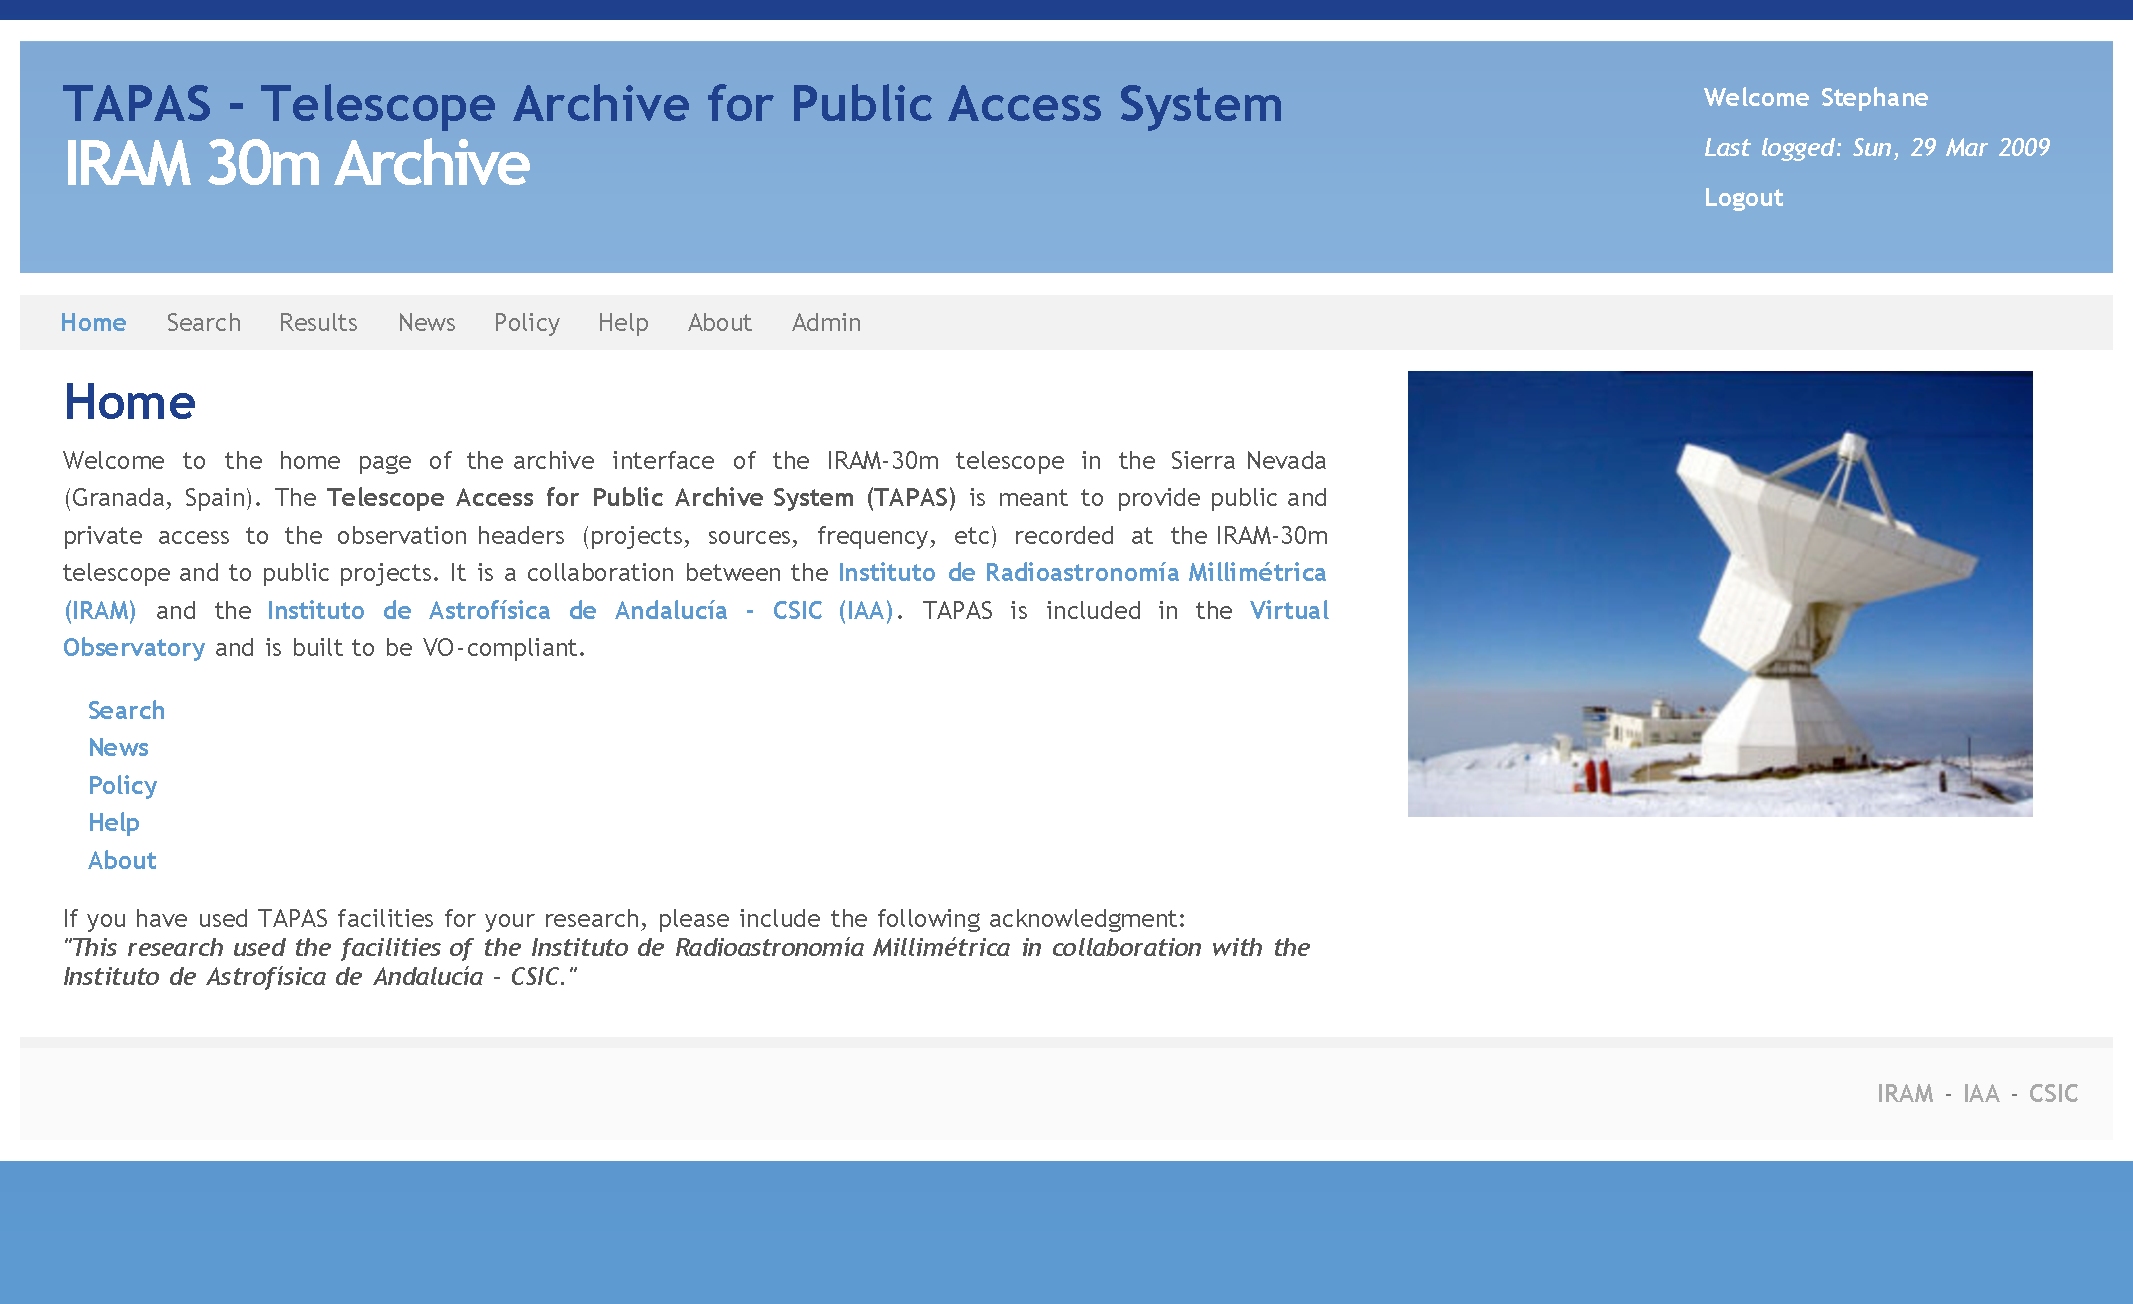
\includegraphics[width=\textwidth]
					{fig/TAPAS_home.pdf}
				\caption[TAPAS home screen]{Home screen of TAPAS,
				with the main functions available from the menu.}
				\label{fig:fig_TAPAS_home}
			\end{figure}
			
			The search form
			---figure~\ref{fig:fig_TAPAS_searchForm}--- allows
			users to perform searches on the Target,
			Provenance.Instrument,
			Provenance.Environment,
			Cha\-rac\-teri\-sa\-tion.Spa\-tial\-Axis,
			Cha\-rac\-teri\-sa\-tion.Tem\-po\-ral\-Axis, and
			Cha\-rac\-teri\-sa\-tion.Spec\-tral\-Axis data models.
			
			For specifying Targets, users can use either widely
			known names, such as those registered by NED for
			astronomical objects, or IRAM project object codes. If
			no suitable name is known, users can provide equatorial
			coordinates\footnote{Right Ascension and Declination
			in the J2000 equinox} in sexagesimal format, and a cone
			angular size in decimal degrees. Object names, when not
			found in the projects, are resolved to coordinates
			using CDS' Sesame service.
			
			The only weather requirement which can be imposed on
			searches is a maximum Opacity, as it can identify those
			datasets which have had a good enough sky for the kind
			of observation we intend to find.
			
			Instrumental requirements include the specification of
			the instrument front-ends, and Spectral\-Axis requirements
			are specified either in the form of frequency ranges,
			of velocity ranges, or the name of the molecular or
			atomic line being observed (i.e. \texttt{CO(1-0)},
			\texttt{HCN}, et cetera).
			
			In addition, TAPAS can be queried by project IDs,
			specially by the PI of the observation, and a Batch
			mode exists by which users can upload a specially
			formatted file which contains a list of names and/or
			position pair coordinates. The names will be resolved by
			either NED or Simbad. If the internal IRAM name is
			to be provided, it should be enclosed by two asterisks
			(\texttt{*}; e.g. \texttt{*M83A*}). The positions are in
			the format \texttt{hh:mm:ss.ss $\pm$dd:mm:ss.ss} (e.g.
			\texttt{12:12:12.12 +30:30:30.30}). Note that right
			ascension coordinates must be given in hours, but
			declination in sexagesimal degrees.
			
			\begin{figure}[tbp]
				\centering
					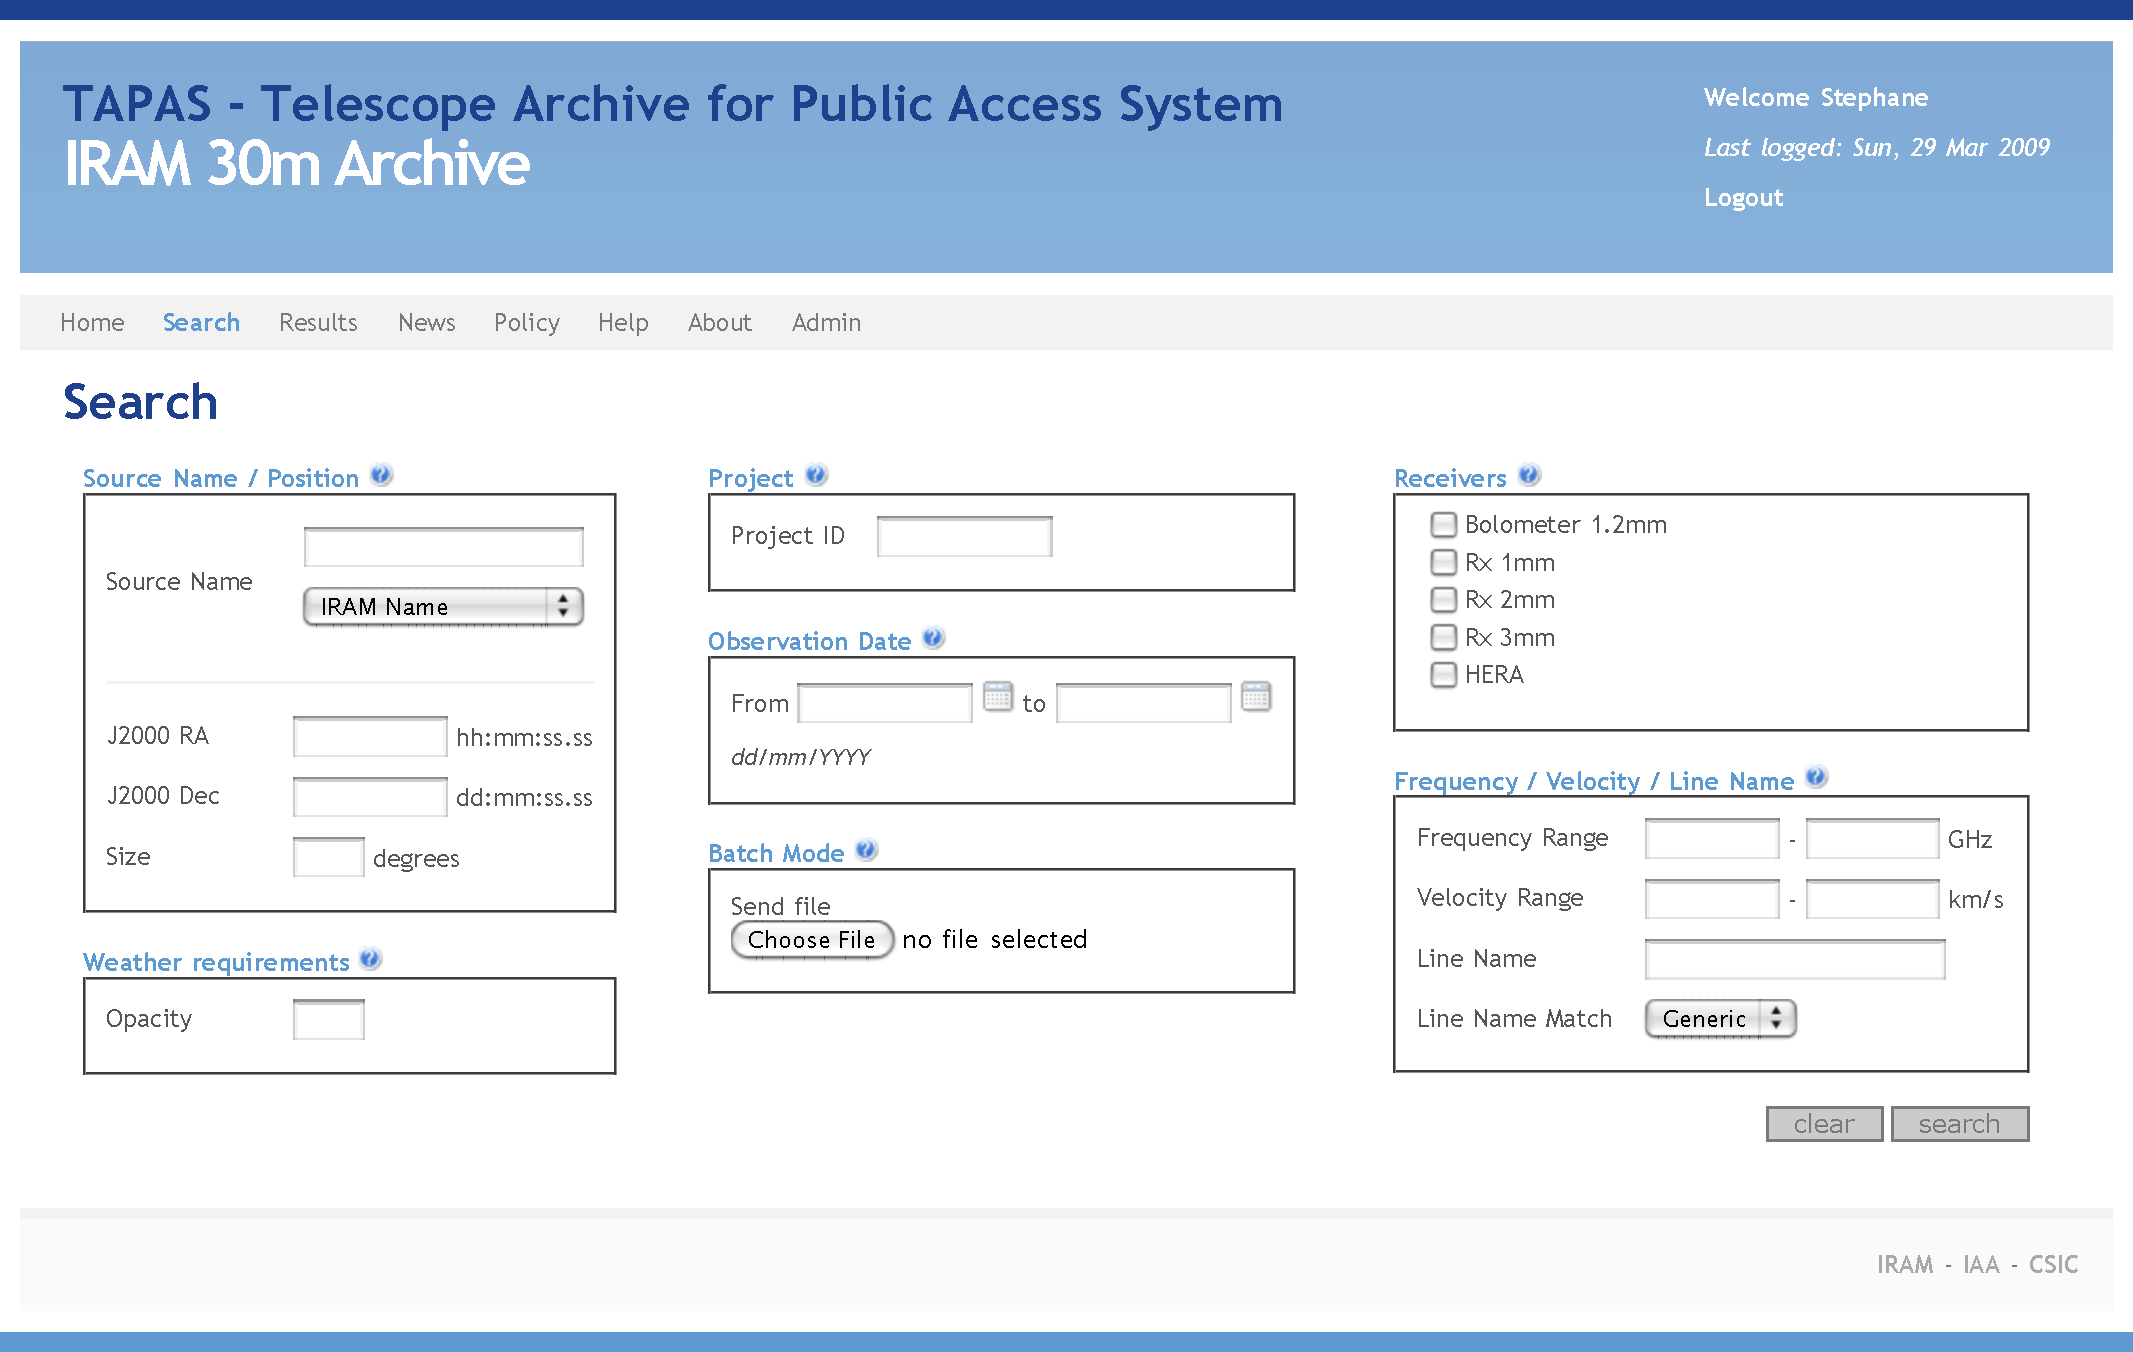
\includegraphics[width=\textwidth]
					{fig/TAPAS_searchForm.pdf}
				\caption[TAPAS search form]
				{Search form of TAPAS. Queries can be performed
				on any of the blocks presented to the user.}
				\label{fig:fig_TAPAS_searchForm}
			\end{figure}
			
			After searching for observations, the results are
			provided in HTML form, but also Comma Separated Values
			(CSV) ASCII files, and VOTables can be generated.
			Even a PDF of the results page can be downloaded
			---see figure~\ref{fig:fig_TAPAS_searchResults}---.
			
			The available header information are the internal
			(IRAM) source name, object equatorial coordinates
			(J2000), project identifier (ID), receiver, sky
			opacity, and time-stamps for the start of the first
			and the latest scans for the observation.
			
			\begin{figure}[tbp]
				\centering
					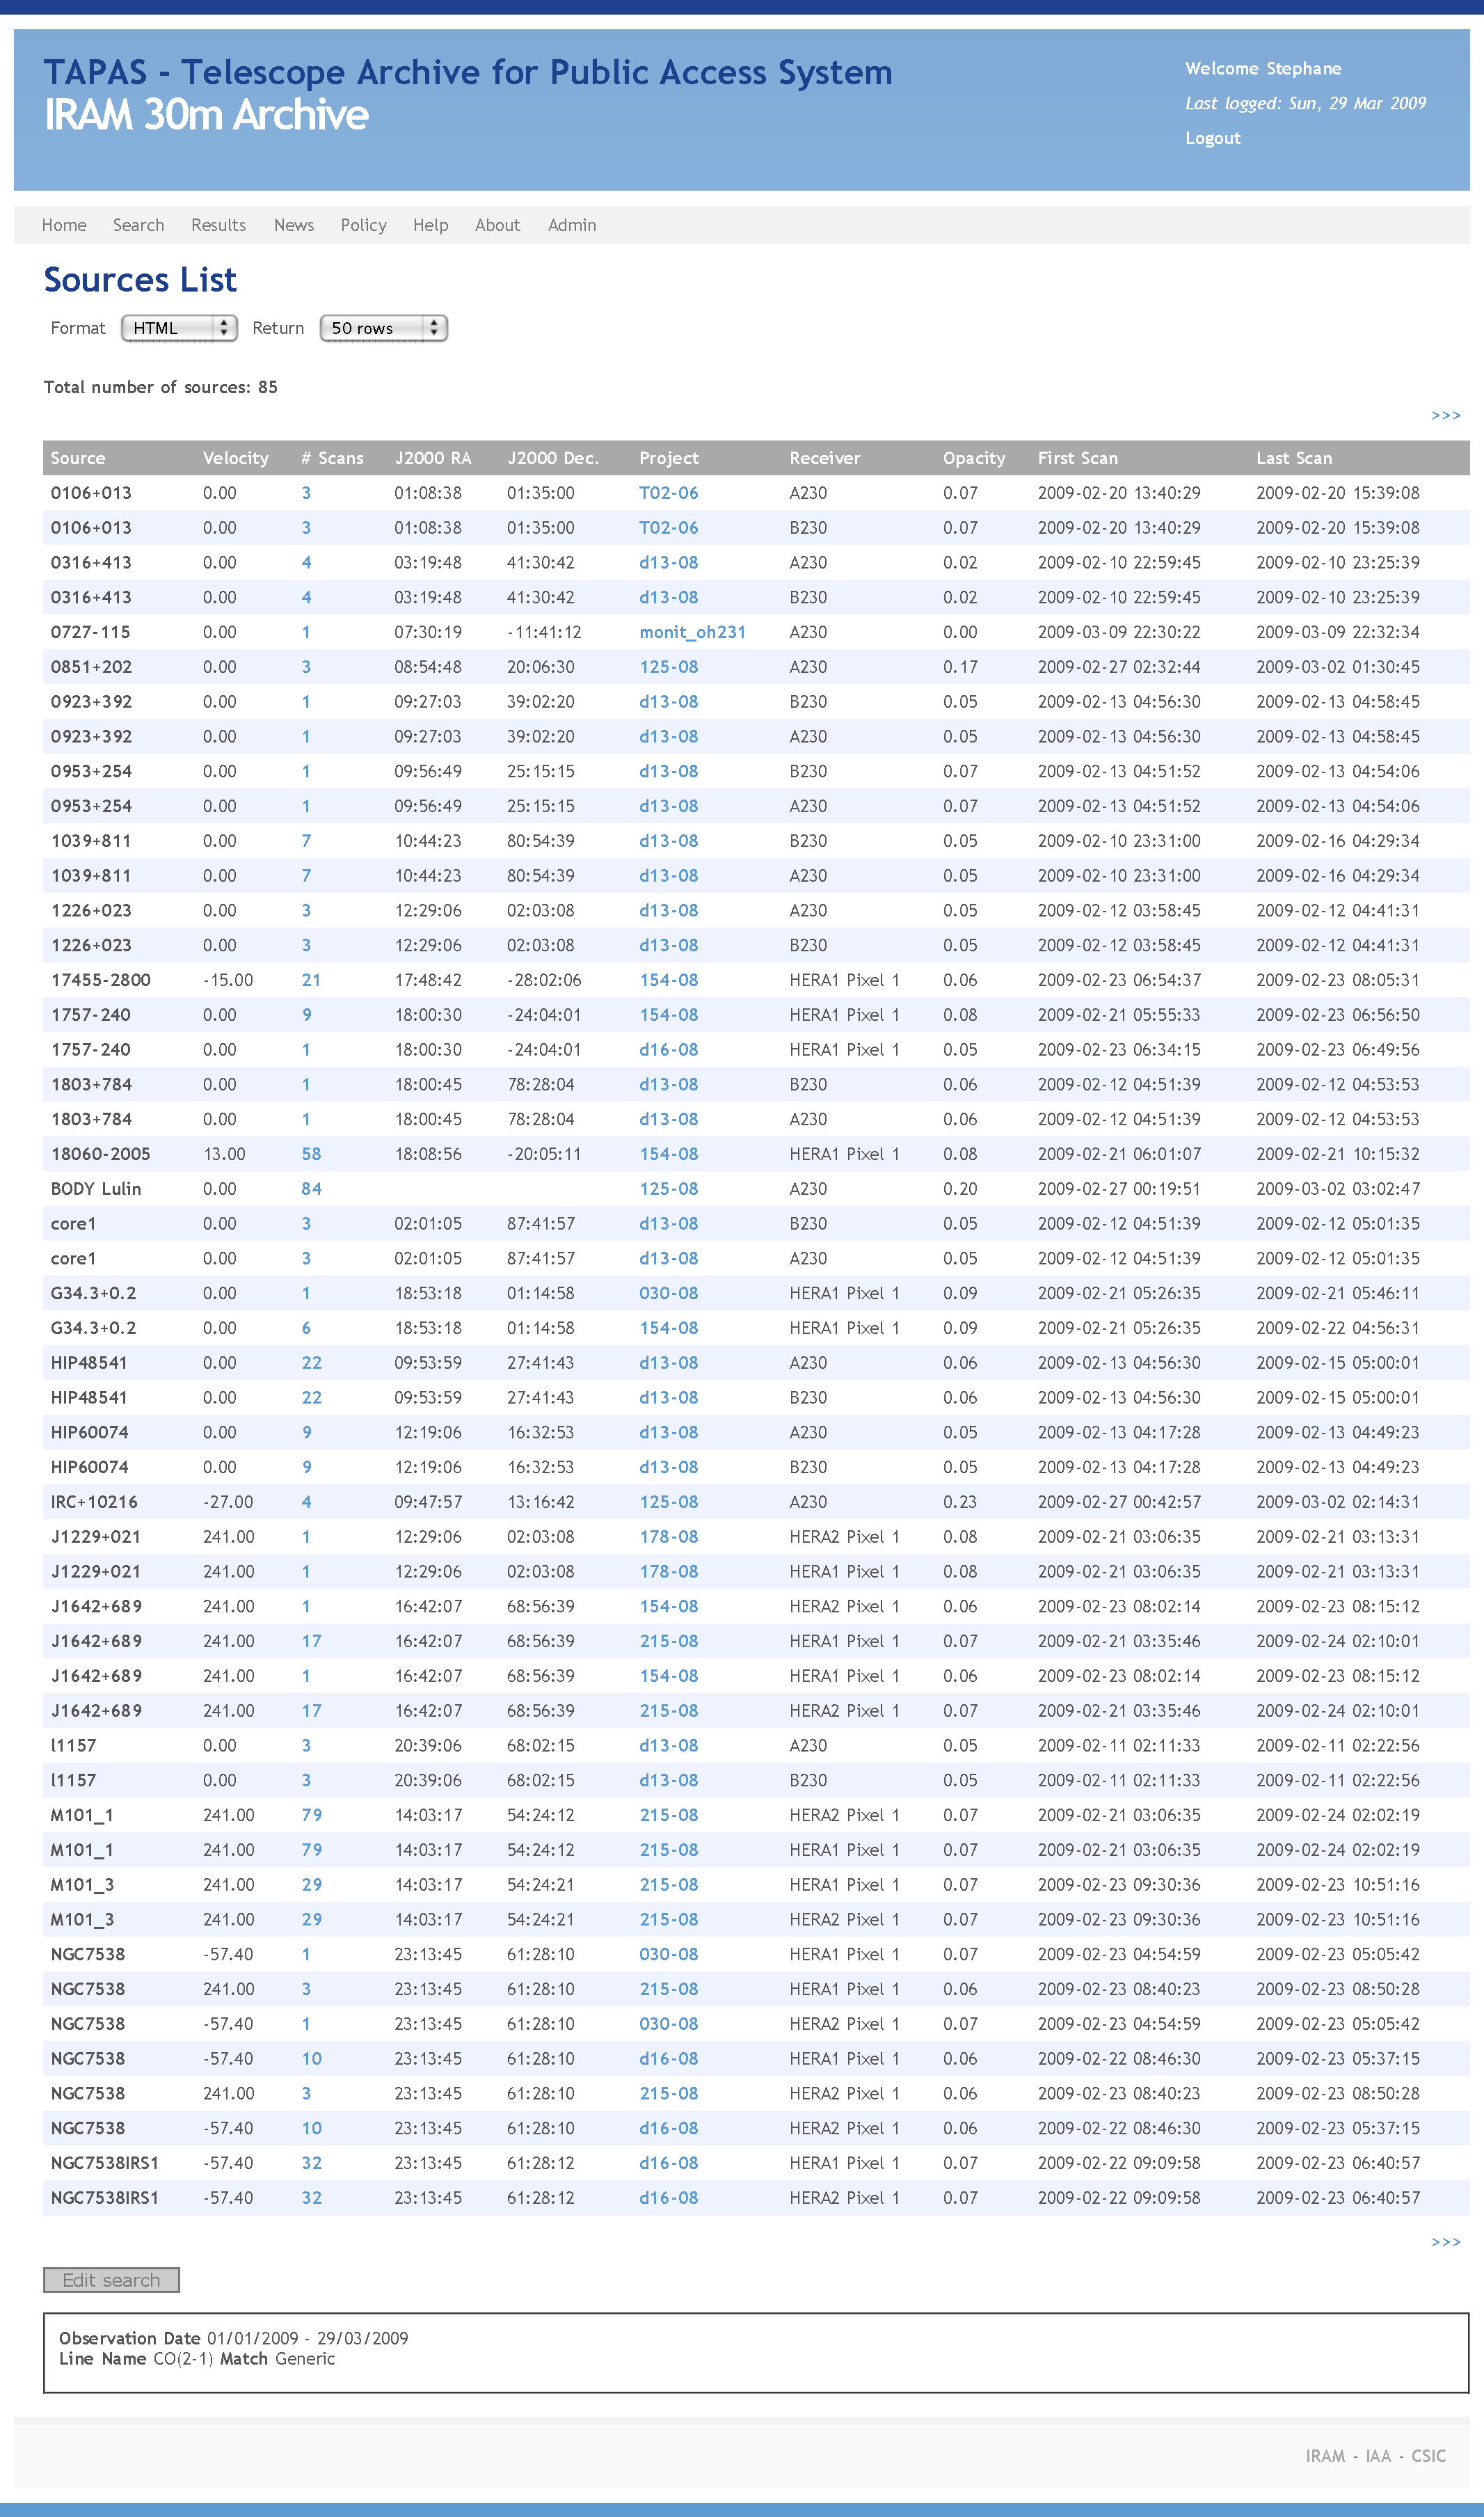
\includegraphics[totalheight=\textheight]
					{fig/TAPAS_searchResults.pdf}
				\caption[TAPAS search results]
				{TAPAS search results. Apart from the result list,
				the actual query is shown at the bottom of the
				results page.}
				\label{fig:fig_TAPAS_searchResults}
			\end{figure}
			
			When the user clicks on the Project link, a new
			page appears with project details ---see
			figure~\ref{fig:fig_TAPAS_projectDetail}---, including
			the time spanned by all project's scans, how many
			scans belong to the project, and how many have been
			performed using the MAMBO bolometer, or the heterodyne
			receivers.
			
			For all project scans, a graph is provided where the
			taumeter reading (from the WeatherTau table) is plotted
			for each scan, giving users a view of the evolution of
			opacity throughout the different project's scans.
			
			\begin{figure}[tbp]
				\centering
					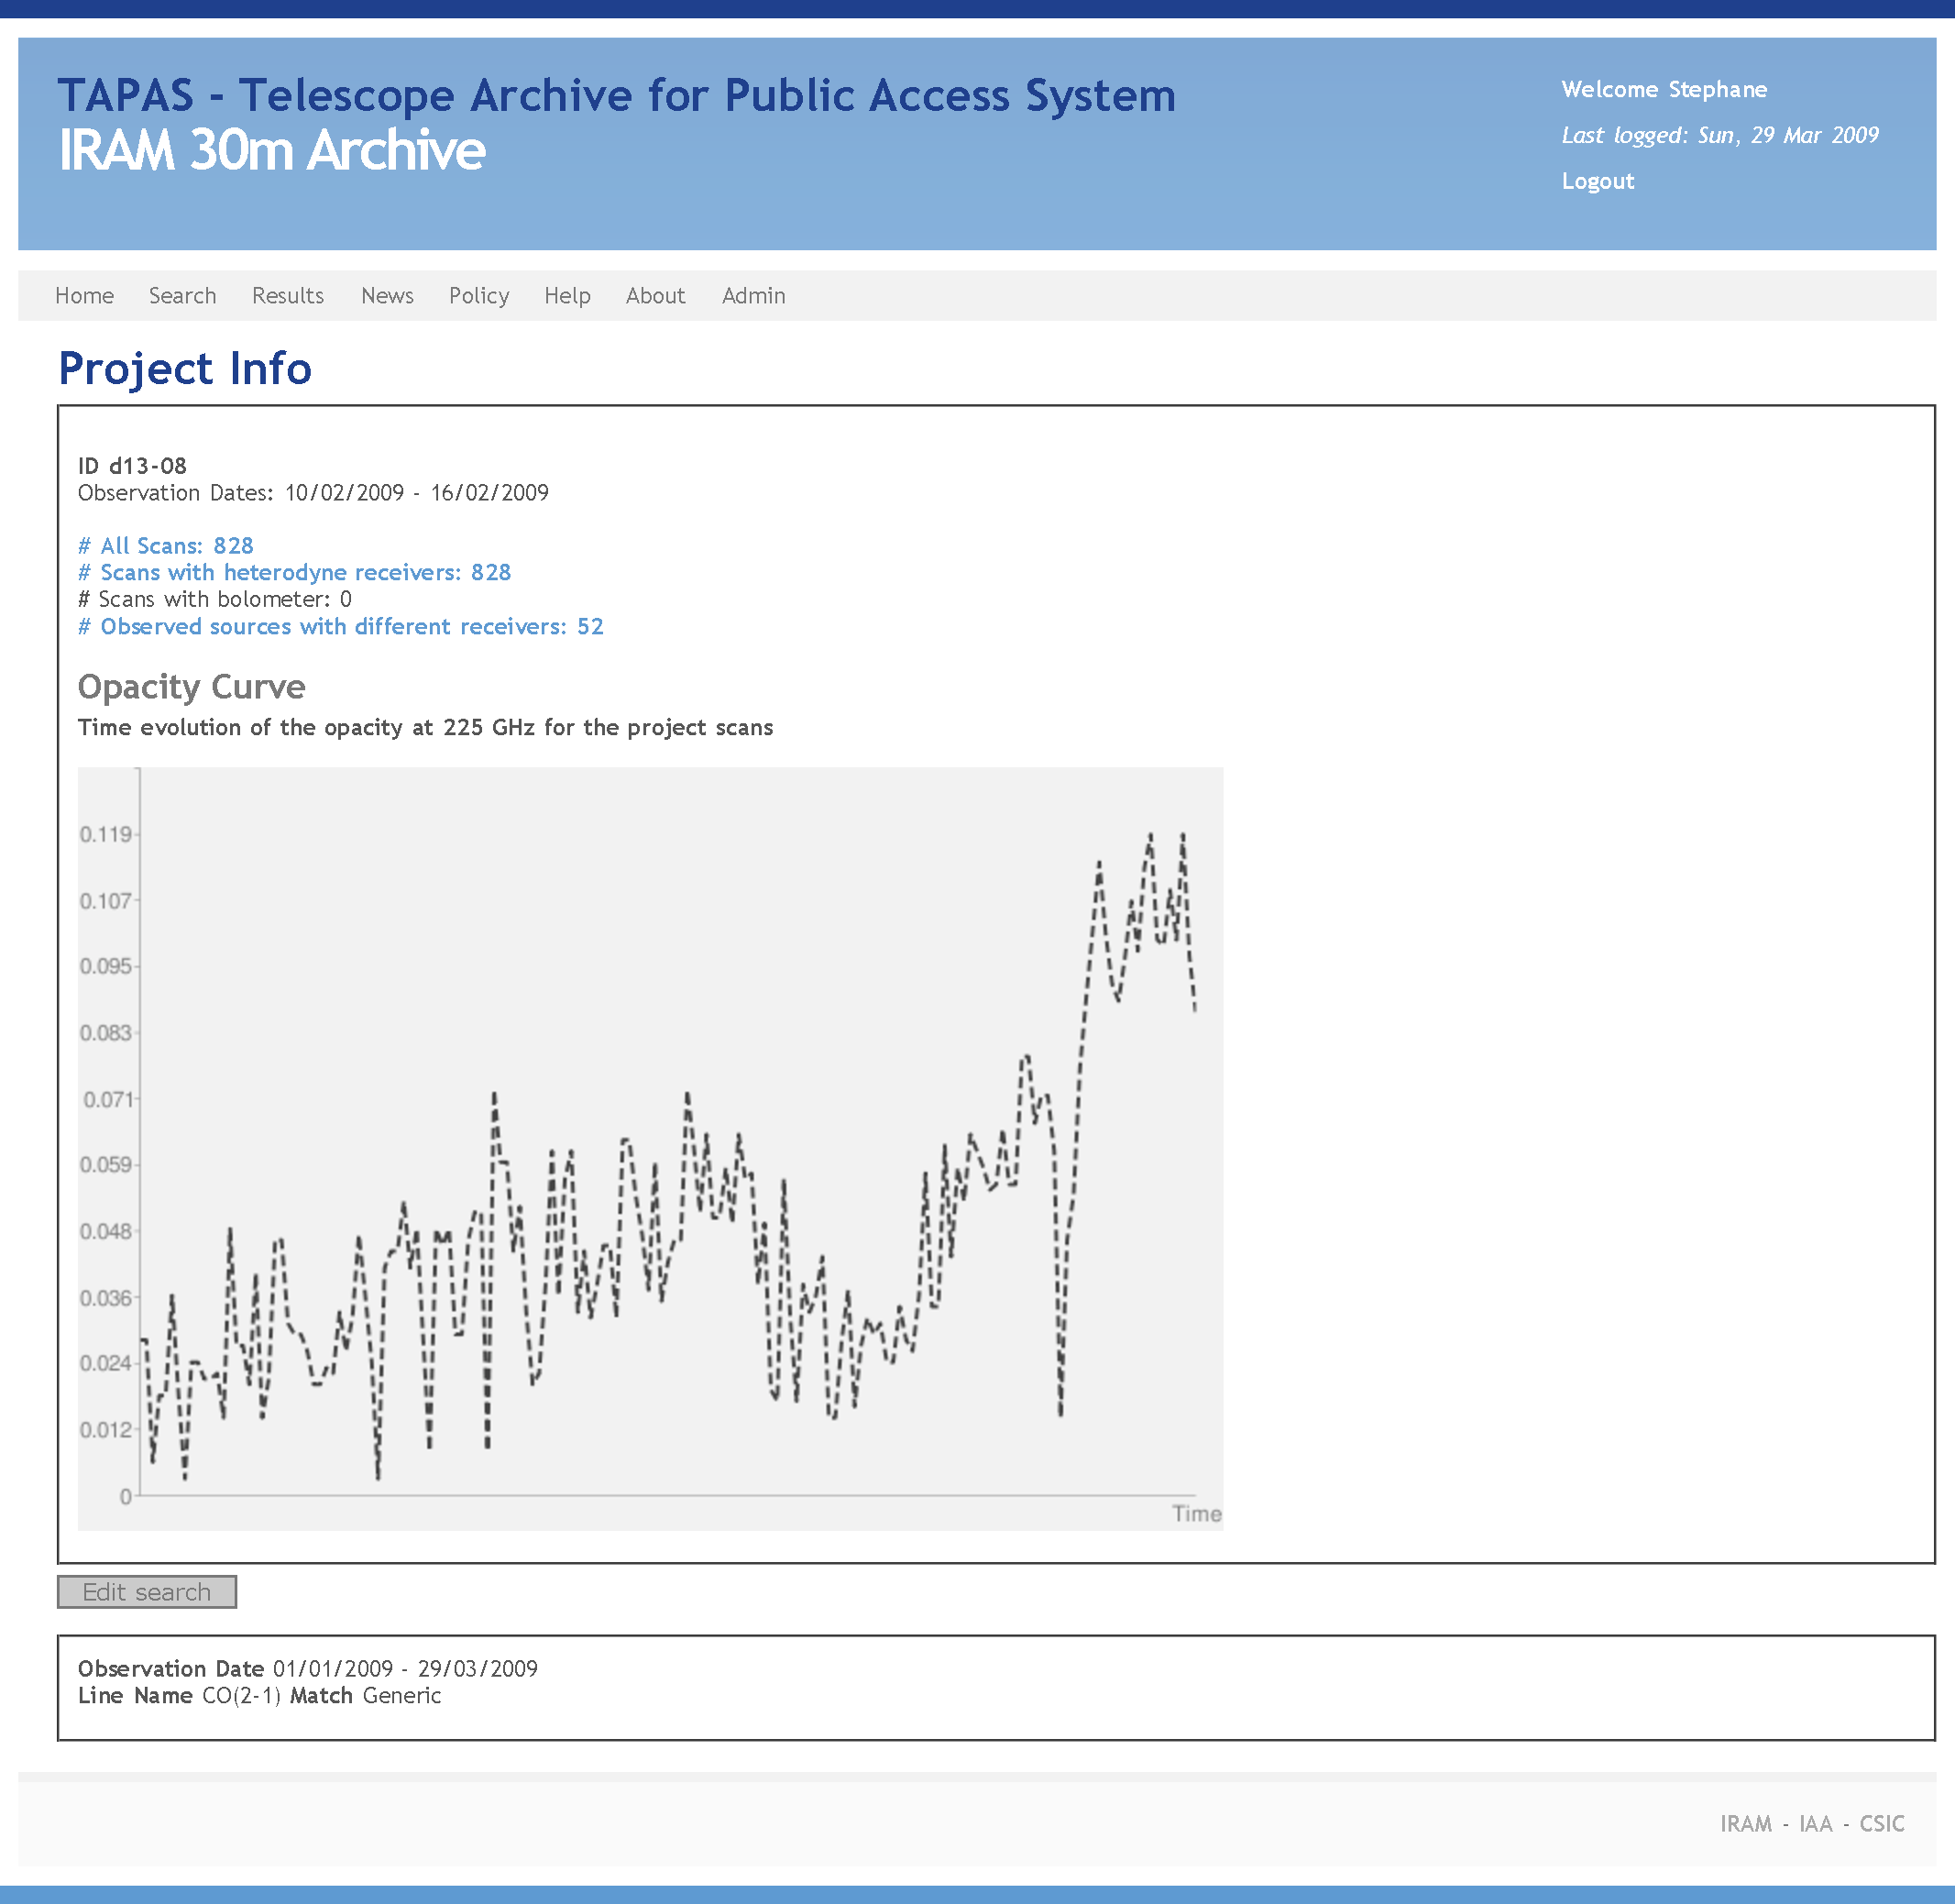
\includegraphics[width=\textwidth]
					{fig/TAPAS_projectDetail.pdf}
				\caption[TAPAS project detail page]
				{TAPAS provides detailed information on projects,
				including access to observations in the project.}
				\label{fig:fig_TAPAS_projectDetail}
			\end{figure}
			
			If users click on the number of scans for
			an observation on the Results page, a detailed view of
			all scans for a given observation is provided
			---see
			figure~\ref{fig:fig_TAPAS_scansPerObservation}---,
			together with the common parameters for all scans:
			project ID, IRAM name of the source, velocity setting,
			equatorial coordinates, equinox, and receiver. This
			list can be also retrieved as HTML, CSV, or VOTable.
			
			\begin{figure}[tbp]
				\centering
					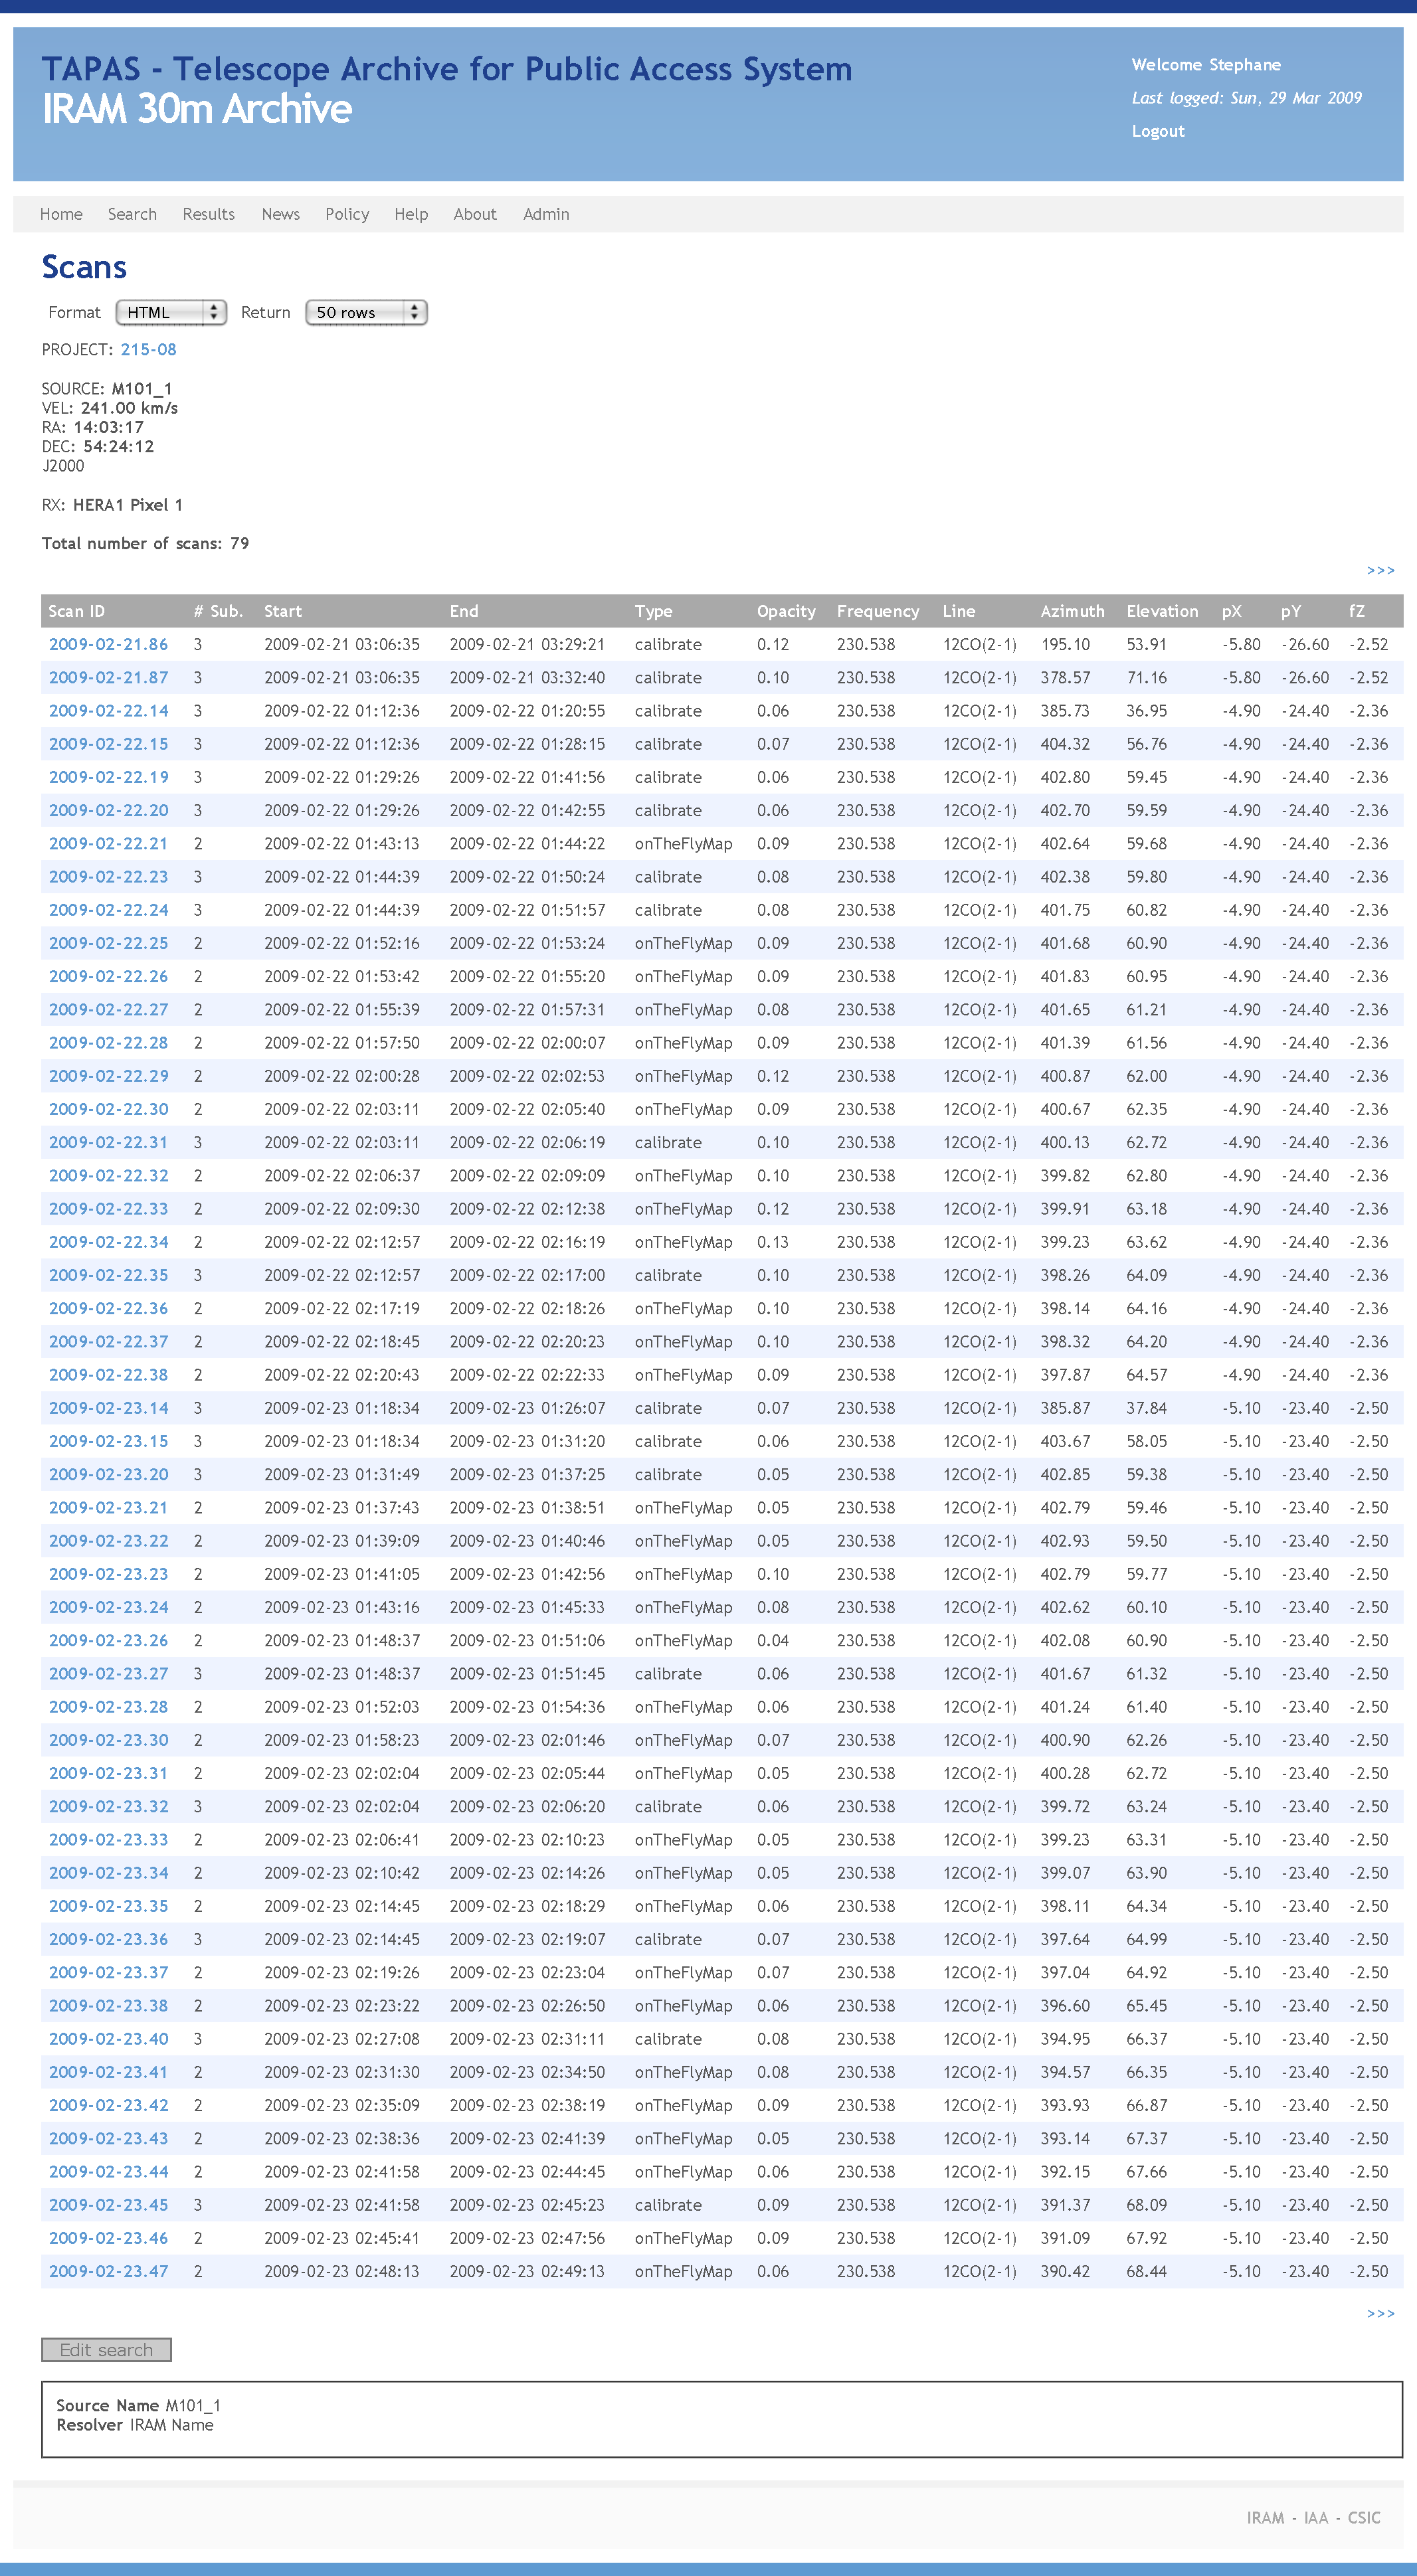
\includegraphics[totalheight=\textheight]
					{fig/TAPAS_scansPerObservation.pdf}
				\caption[TAPAS observation scans]
				{TAPAS provides a list of all of the scans
				composing an observation.}
				\label{fig:fig_TAPAS_scansPerObservation}
			\end{figure}
			
			If a particular scan is clicked, the information
			for that scan is shown ---see
			figure~\ref{fig:fig_TAPAS_scanDetails}---, and
			obtains a link to the data (if available as per
			IRAM policy), Characterisation.TemporalAxis
			information (observation length, start, and stop),
			Target information (source name, coordinates),
			Provenance.Environment (weather conditions),
			Provenance.Instrument (antenna azimuth and elevation,
			pointing and focus corrections, observing mode,
			calibration settings, offsets, front-ends and back-ends), 
			Provenance.Processing (software version, and calibration
			settings), and Characterisation.SpectralAxis (spectral
			line).
			
			\begin{figure}[htbp]
				\centering
					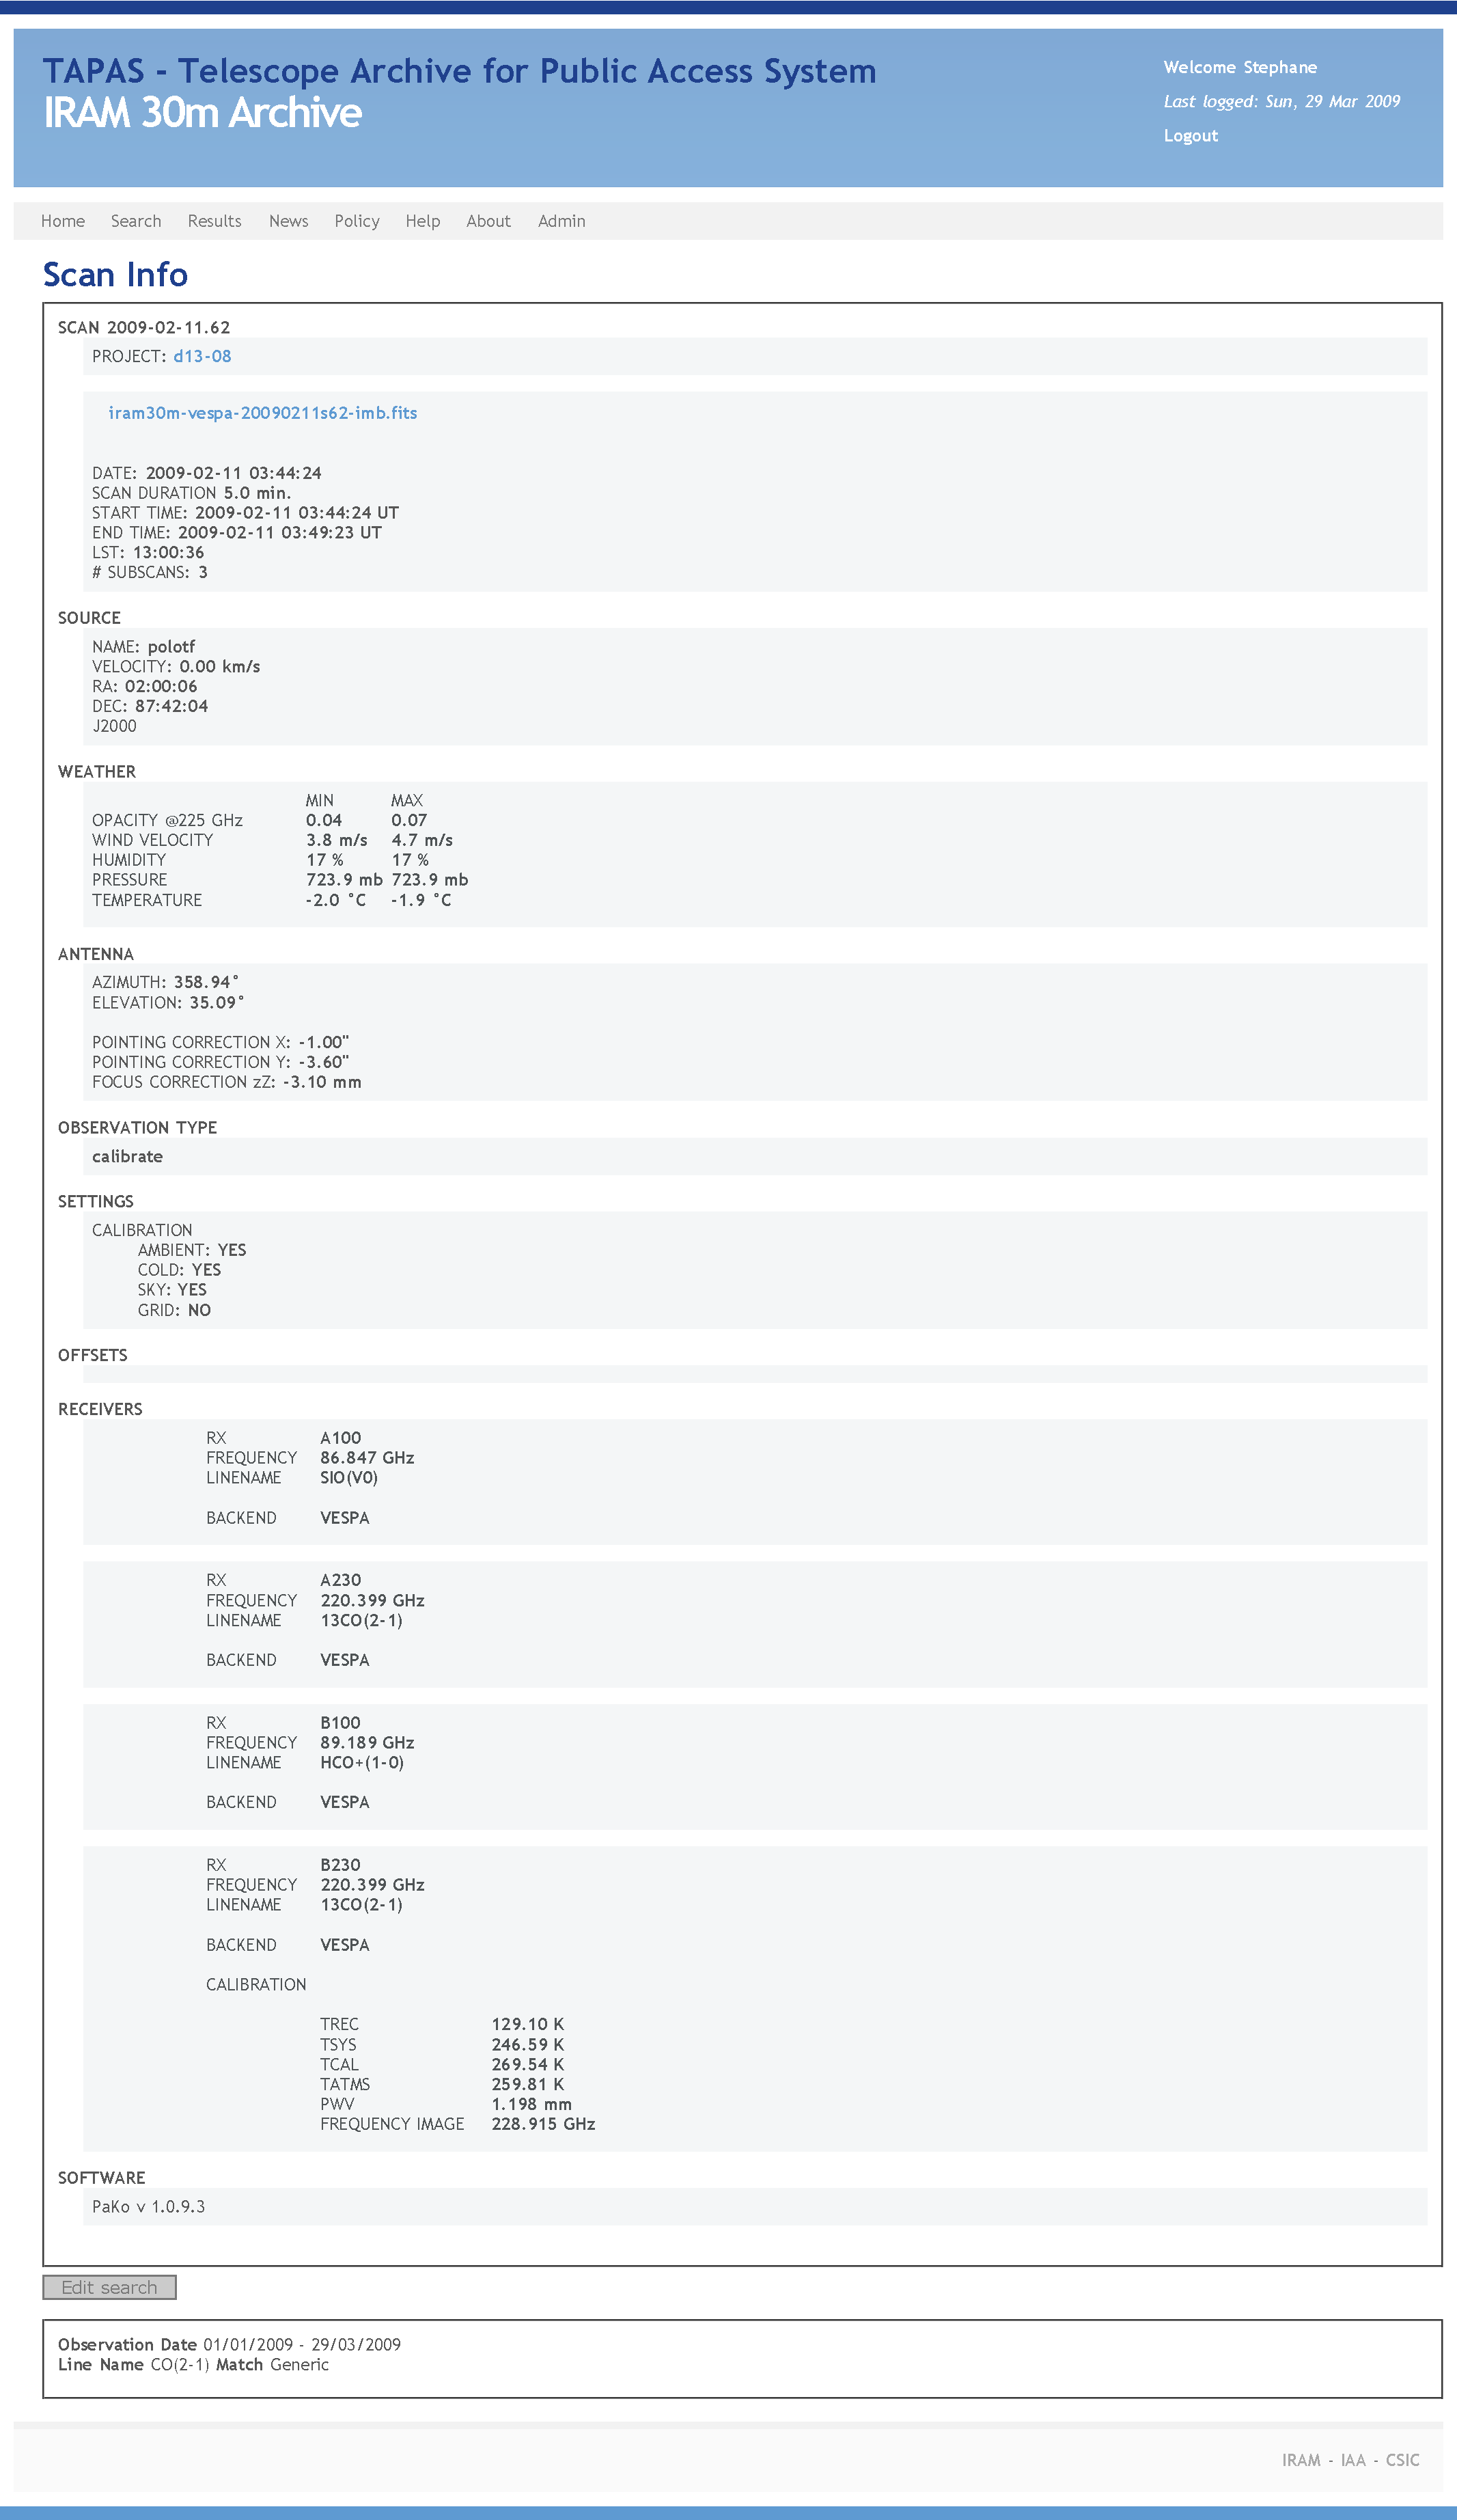
\includegraphics[totalheight=\textheight]
					{fig/TAPAS_scanDetails.pdf}
				\caption[TAPAS scan detail for an on-off
				calibration]
				{Details of an on-off calibration scan in TAPAS.}
				\label{fig:fig_TAPAS_scanDetails}
			\end{figure}
			
			For different observing modes, the scan information
			provided is different. Compare
			figure~\ref{fig:fig_TAPAS_scanDetails} with
			figure~\ref{fig:fig_TAPAS_scanDetailsOTF}. The
			data models are the same, but the information
			provided is different, corresponding to the differences
			in observation setup (Provenance.Instrument), and
			spatial and temporal coverage in the Characterisation.
			
			\begin{figure}[tbp]
				\centering
					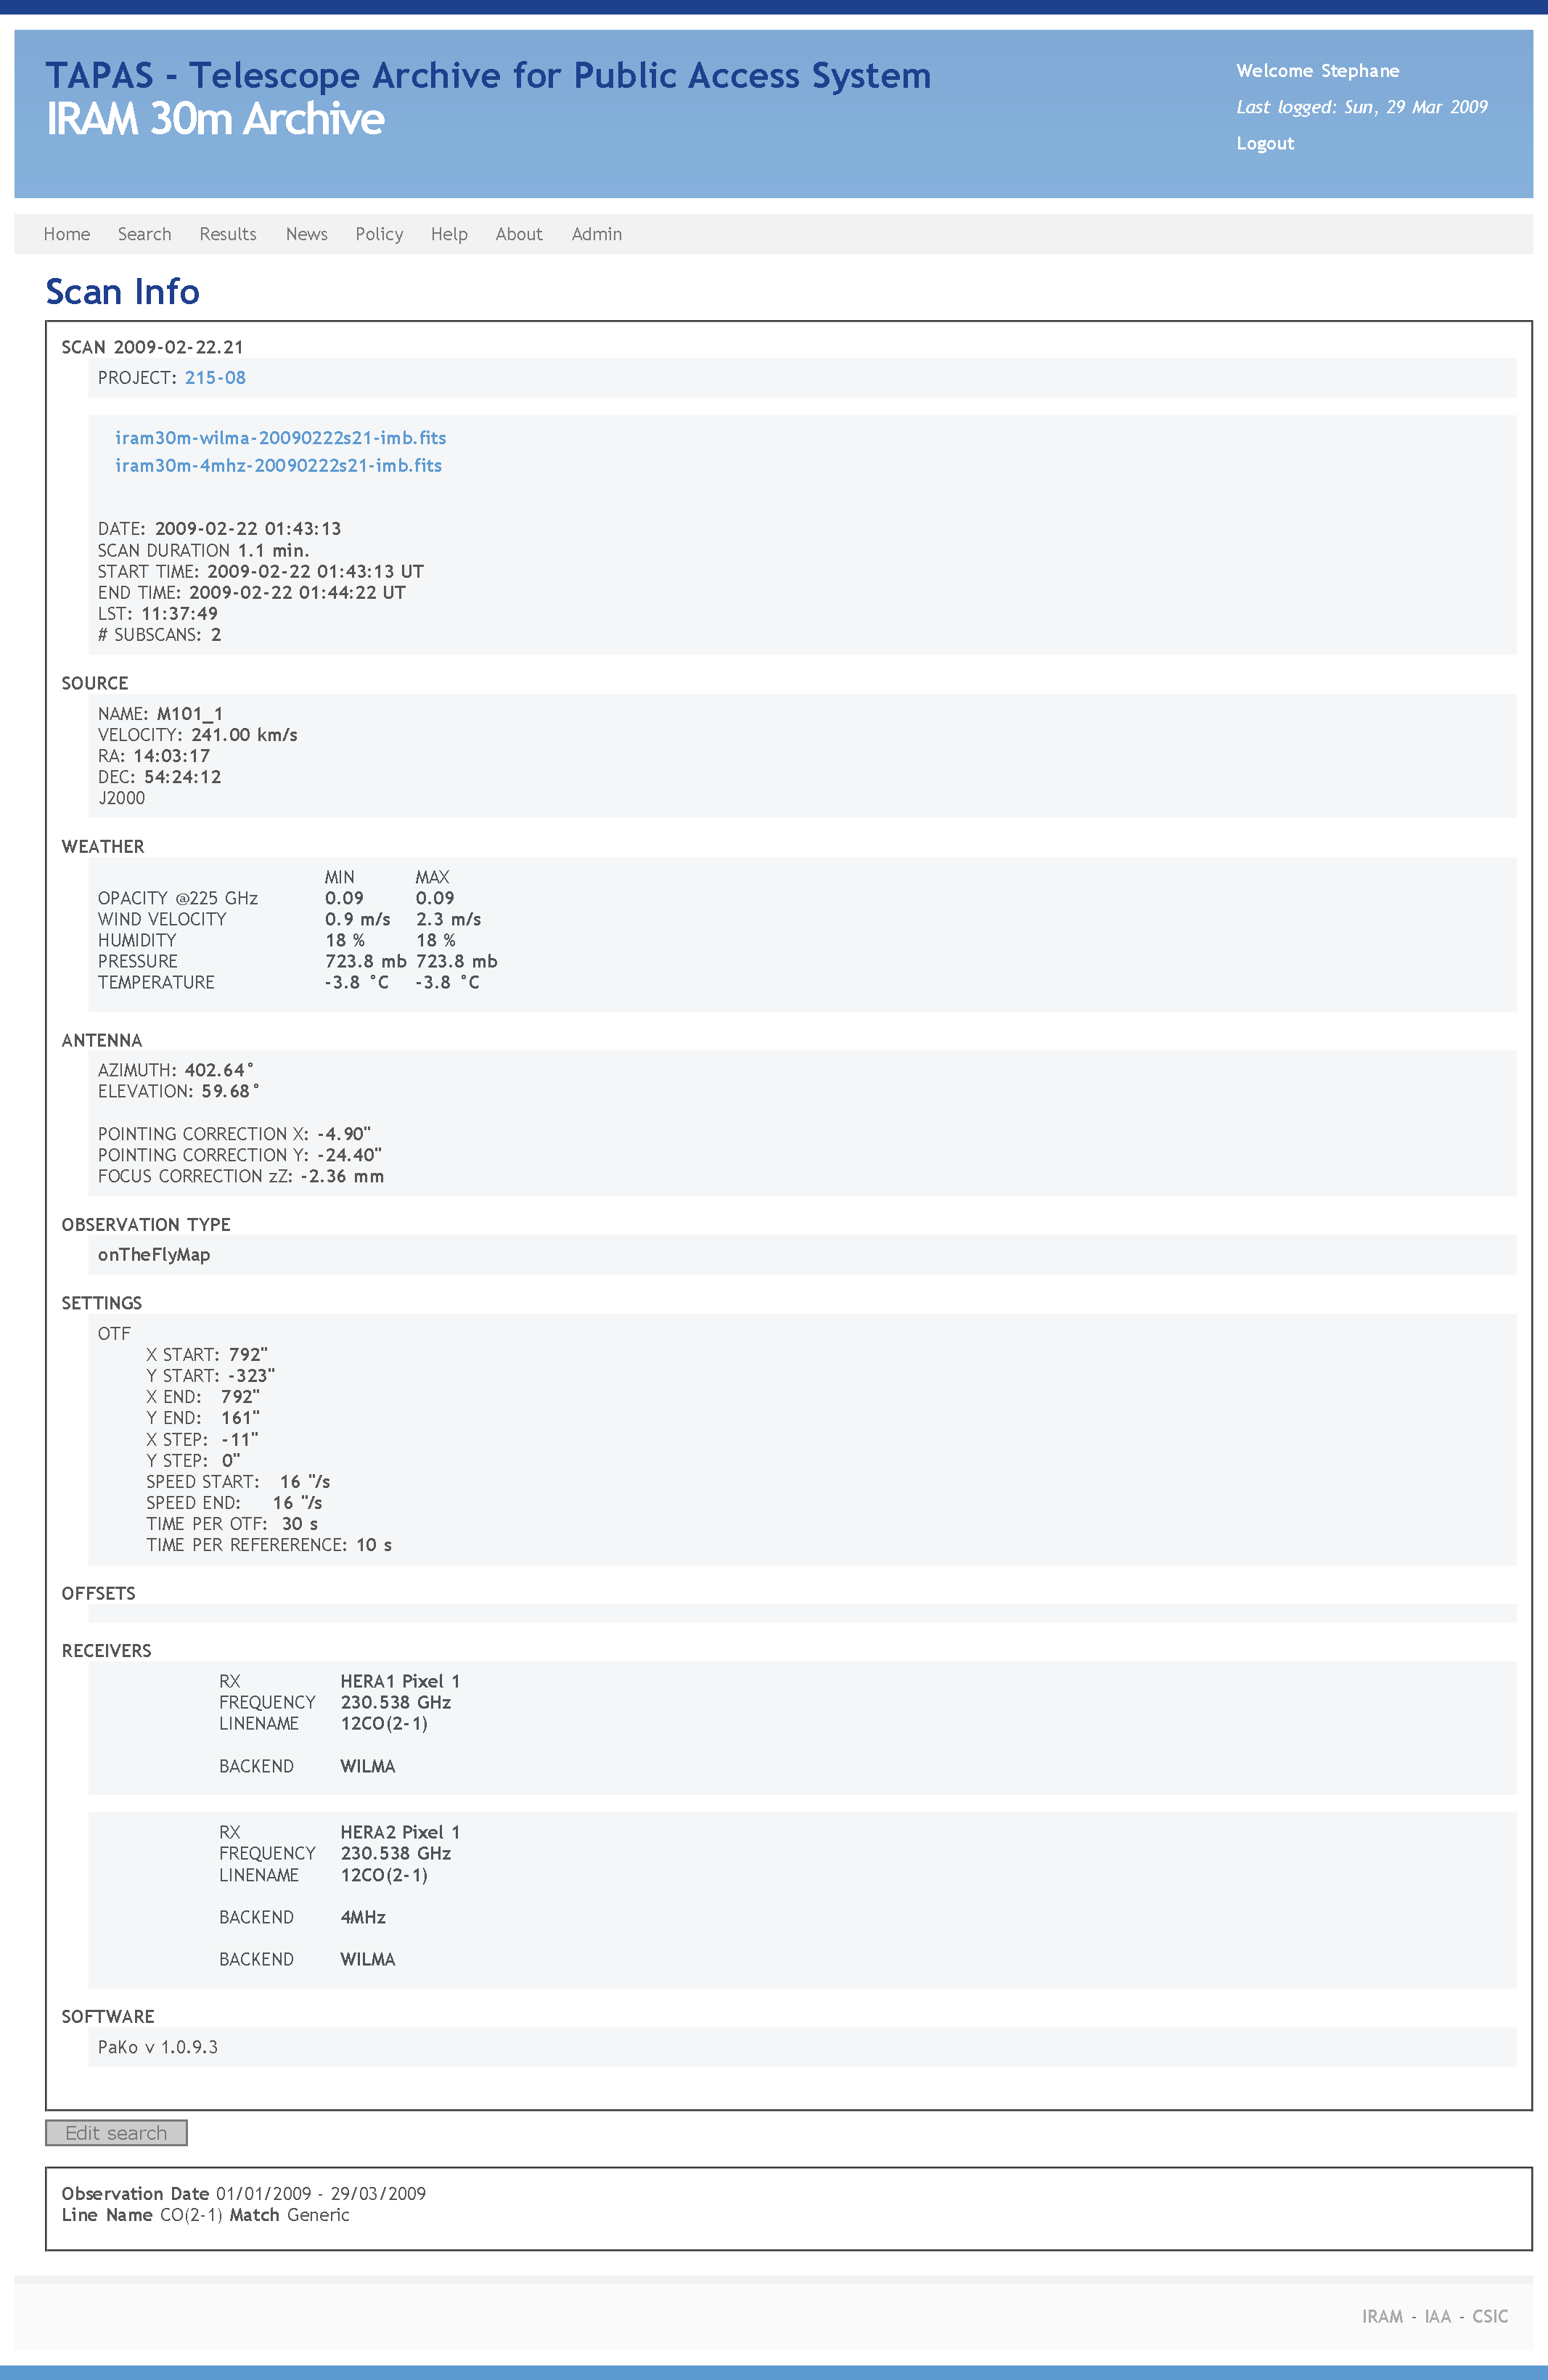
\includegraphics[totalheight=\textheight]
					{fig/TAPAS_scanDetailsOTF.pdf}
				\caption[TAPAS scan detail for an OTF map]
				{Details for a scan belonging to an OTF map.}
				\label{fig:fig_TAPAS_scanDetailsOTF}
			\end{figure}
			
			Finally, figure~\ref{fig:fig_TAPAS_projectSources}
			shows a listing of all sources observed for a given
			project, accessible from the Project details page.
			
			\begin{figure}[tbp]
				\centering
					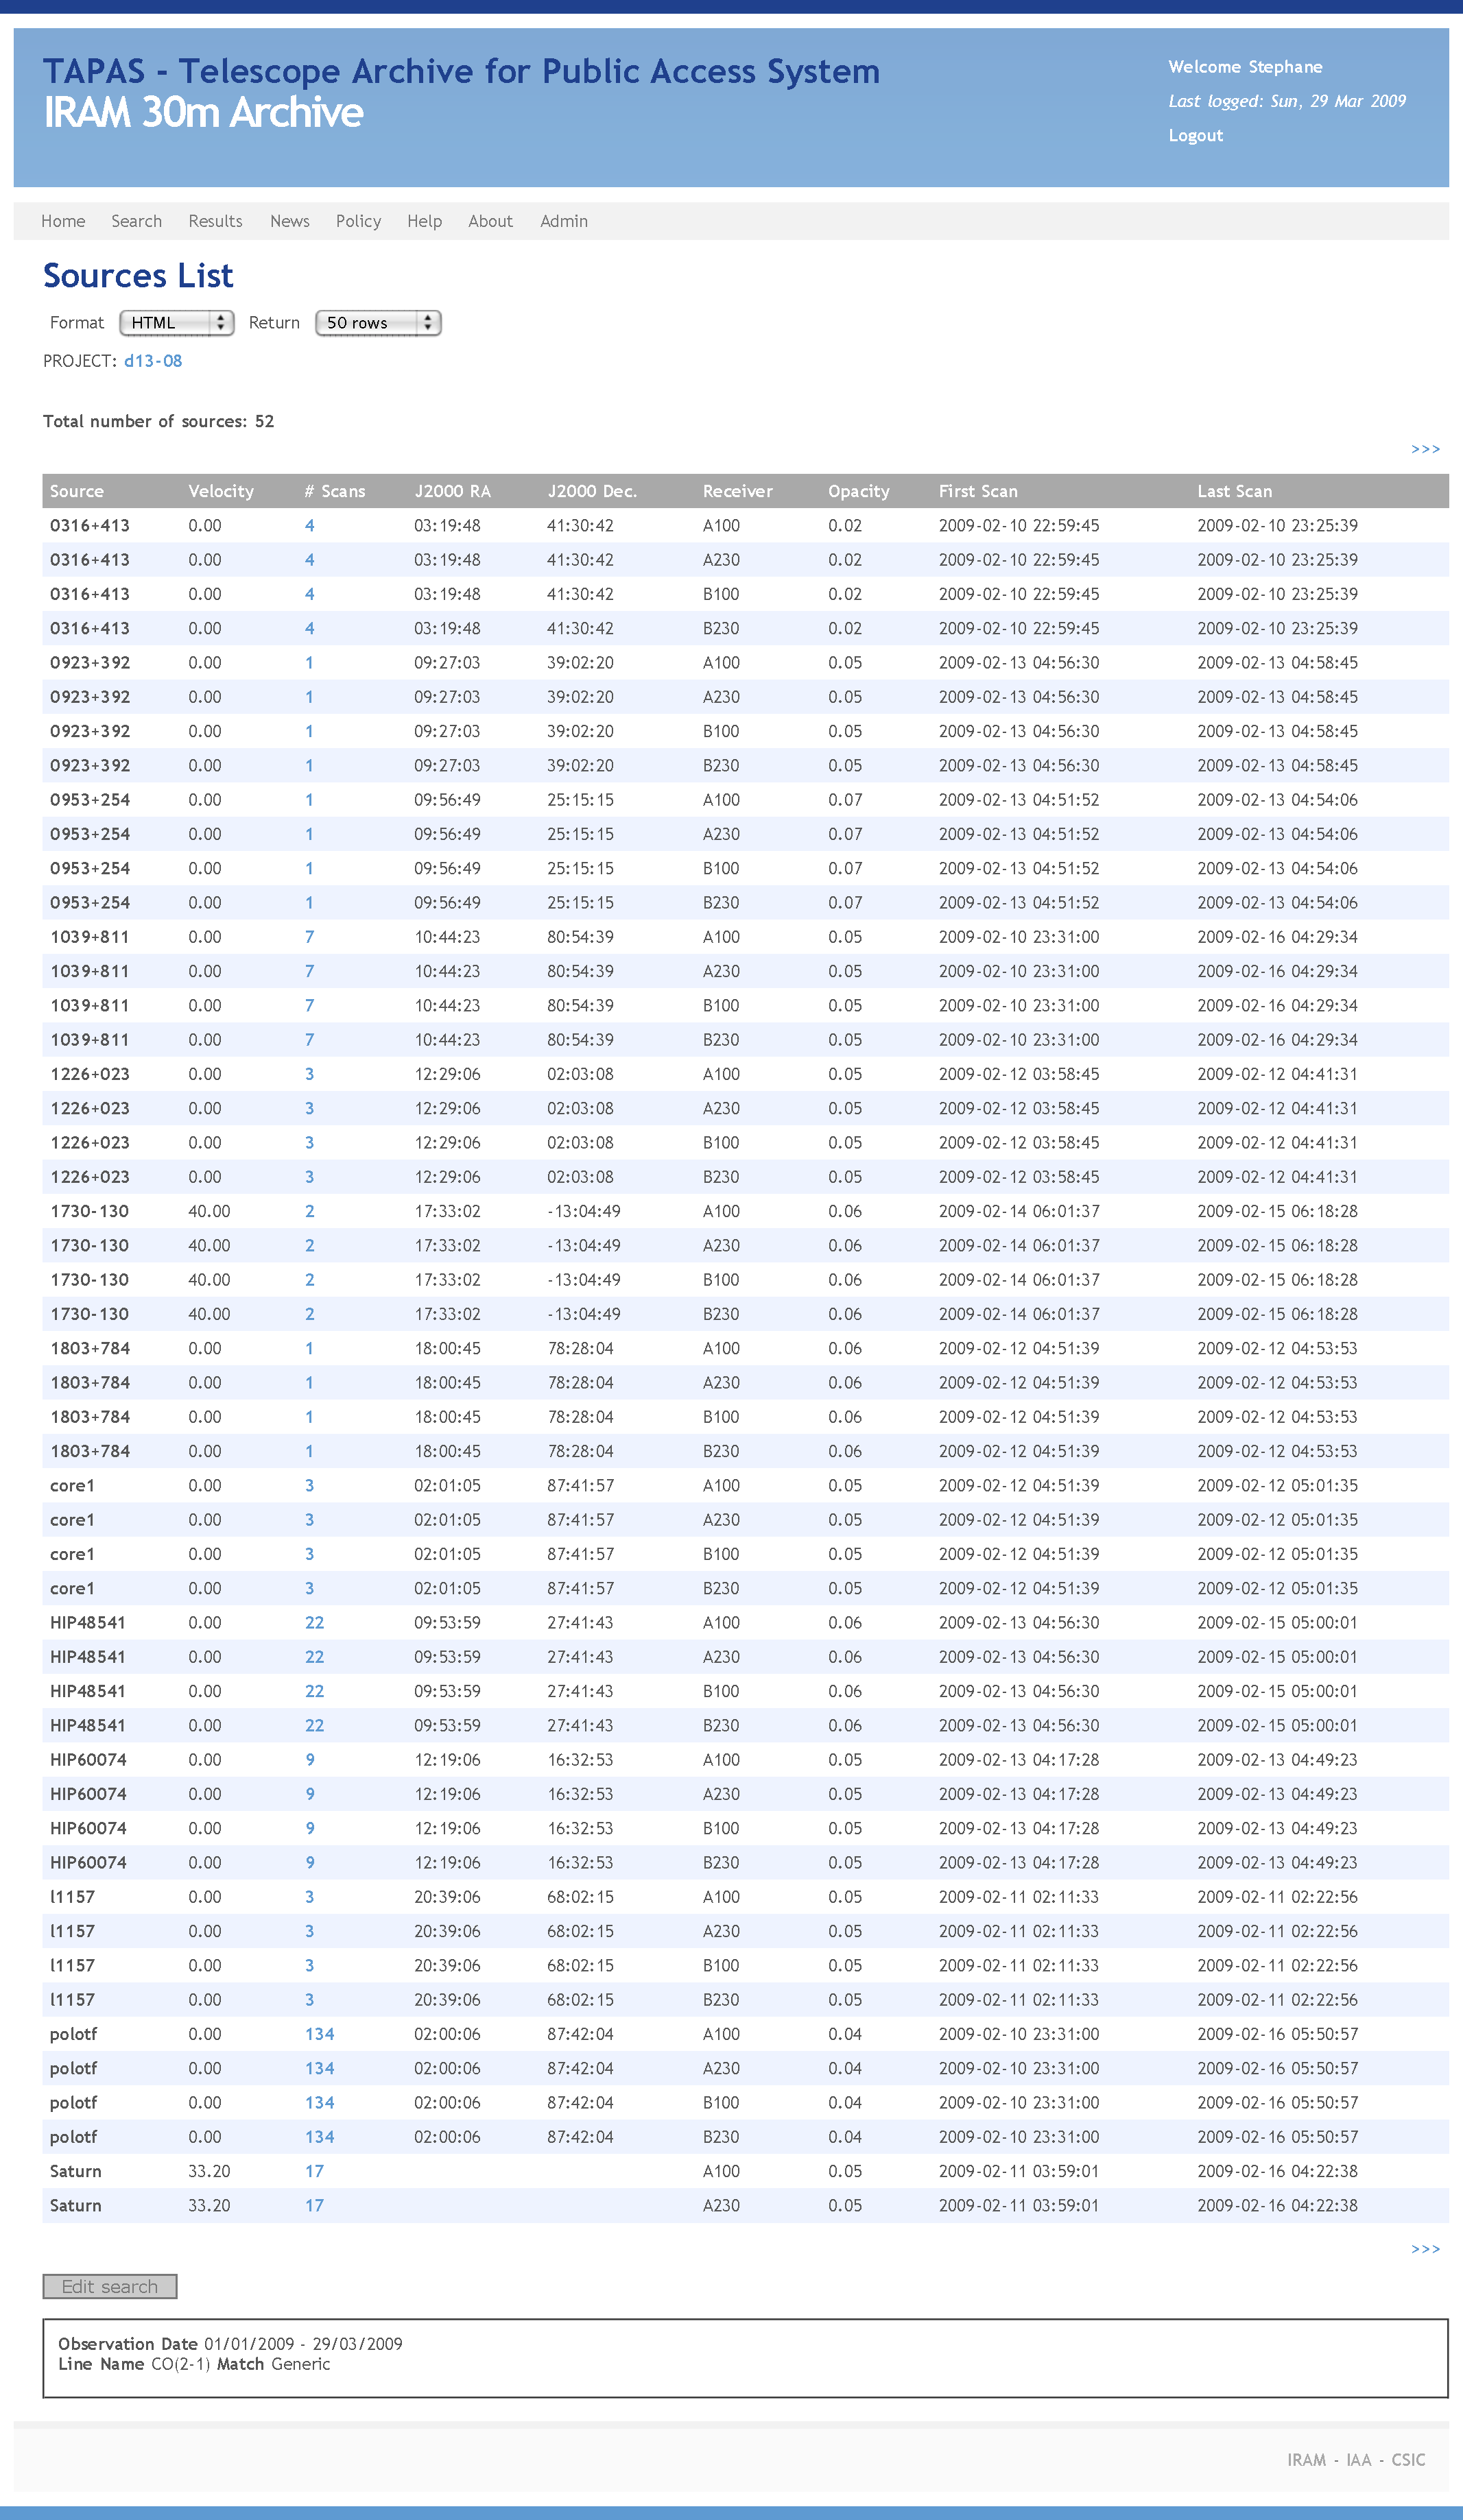
\includegraphics[totalheight=\textheight]
					{fig/TAPAS_projectSources.pdf}
				\caption[TAPAS project sources]{TAPAS
				provides access to all sources observed in
				a given project.}
				\label{fig:fig_TAPAS_projectSources}
			\end{figure}
			
			Apart from the searching capabilities, the TAPAS
			web site provides links to help on the TAPAS
			user interface, and includes a link to the IRAM policy
			statement, as can be seen in
			figure~\ref{fig:fig_TAPAS_policy}.
			
			This is the official TAPAS policy statement:
			
			\begin{adjustwidth}{\parindent}{\parindent}
				\emph{TAPAS contains header information of all
				astronomical data taken [with the IRAM~30m antenna]
				after 01/01/2009. TAPAS does not contain any
				astronomical heterodyne or bolometer data. However,
				TAPAS provides the possibility to link the header
				data of individual scans to FITS files containing
				the uncalibrated astronomical data. TAPAS provides
				a Virtual Observatory facility for query and
				retrieval of header data.}
				
				\emph{Access rights to any astronomical data in TAPAS
				depend on the project. The PI and IRAM decide when
				to make astronomical data public. For all projects,
				after a proprietary period of one year, a subset of
				header data will be made accessible via web
				interfaces and search tools. IRAM staff have
				immediate and unrestricted access to all header
				data. For large programs, access to all data will
				be granted after a 18 months proprietary period.
				The proprietary period starts when the last
				observations of a given project are finished.}
			\end{adjustwidth}
			
			
			
			%\begin{figure}[tbp]
			%	\centering
			%		\includegraphics[width=\textwidth]
			%		{fig/TAPAS_searchResultsCoords.pdf}
			%	\caption[TAPAS results for a coordinate search]
			%	{Results for a coordinate search within TAPAS.
			%	See the query at the bottom of the result page.}
			%	\label{fig:fig_TAPAS_searchResultsCoords}
			%\end{figure}
			
			\begin{figure}[tbp]
				\centering
					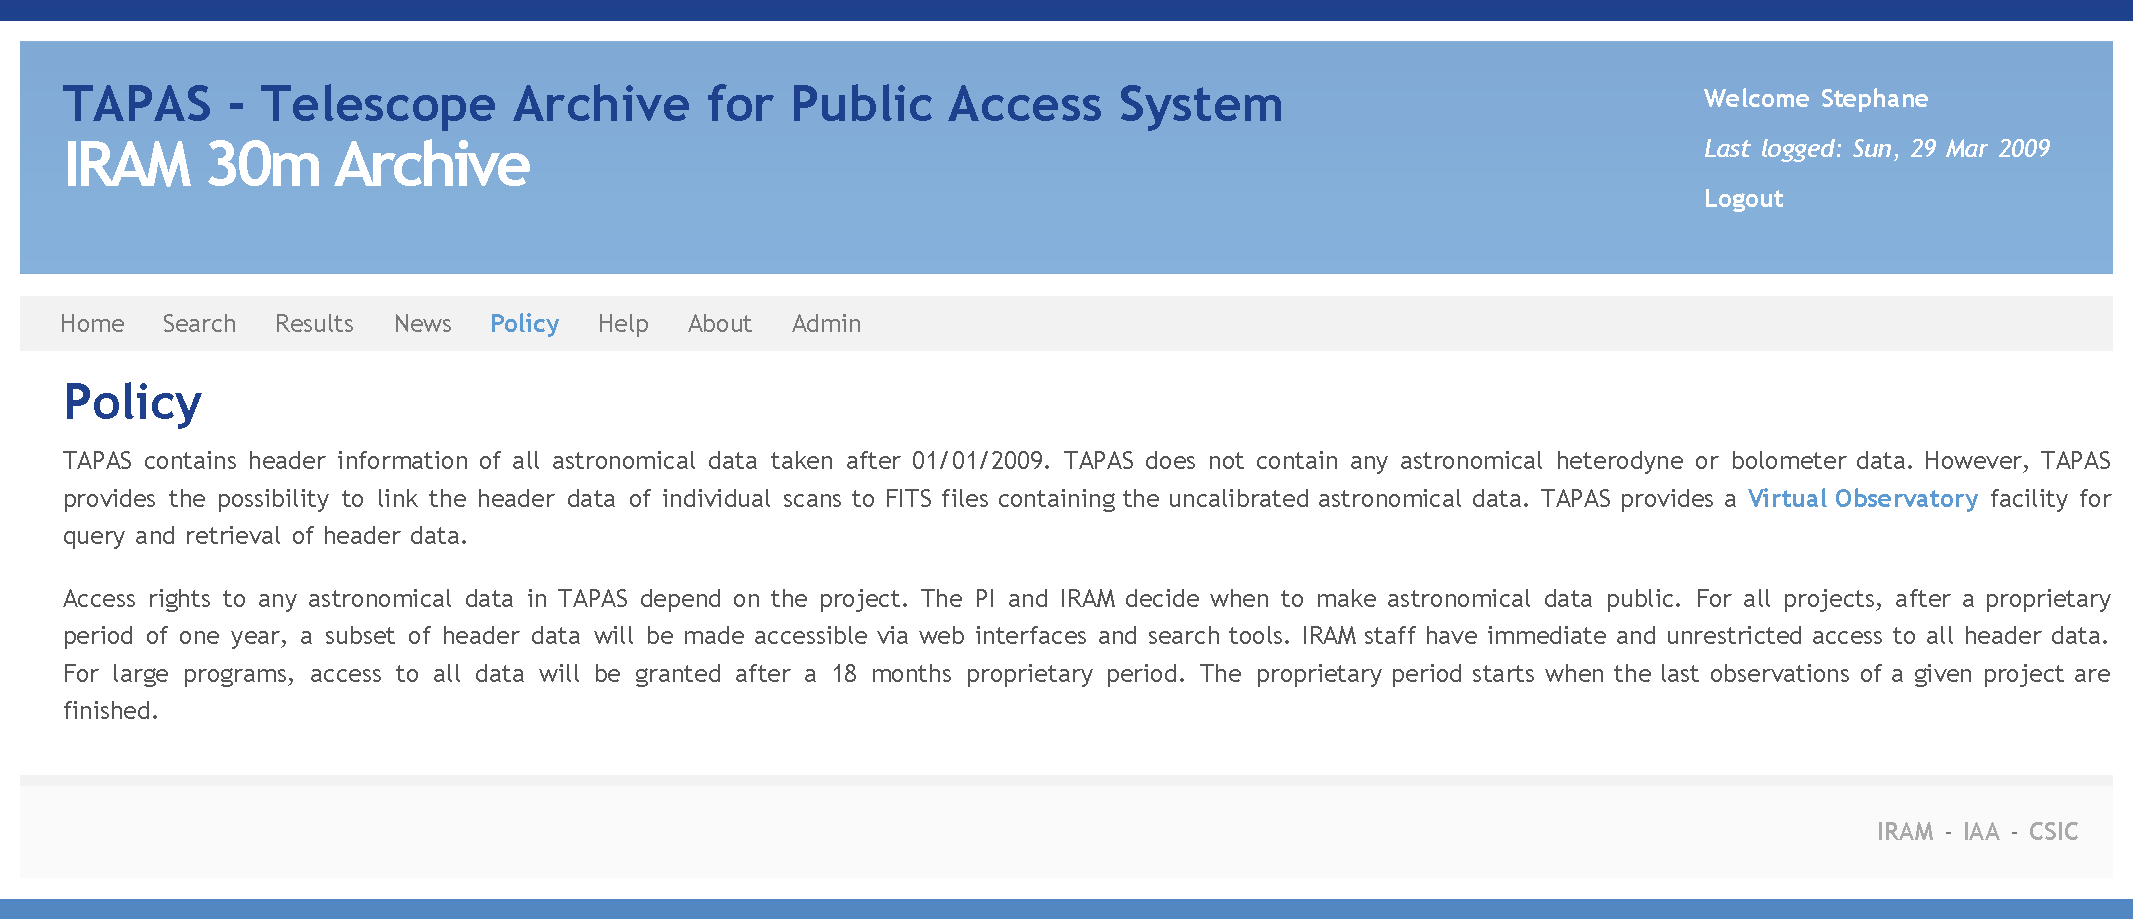
\includegraphics[width=\textwidth]
					{fig/TAPAS_policy.pdf}
				\caption[TAPAS policy]
				{TAPAS policy, as specified by the IRAM.}
				\label{fig:fig_TAPAS_policy}
			\end{figure}
			
			The TAPAS archive has been led by Lourdes
			Verdes-Montenegro (IAA-CSIC), as PI of the coordinated
			project, and Rainer Mauersberger (IRAM), as co-PI for
			the project and leader for the IRAM part, with
			Stéphane Leon (IRAM) as the lead scientist.
			
			On the development part, the development and design
			of the TAPAS archive infrastructure, data models, and
			interfaces has been the responsibility of the IAA-CSIC
			team, while integration issues have been solved by the
			IRAM team.
			
			In particular, the data model was developed by Juan de
			Dios Santander Vela (IAA-CSIC) from the RADAMS, and it
			was adapted by Víctor Espigares (IAA-CSIC) to Django.
			Victor Espigares is also responsible for the
			Data-filler ---the Archive Infrastructure module in
			figure~\ref{figDss63ArchiveArchitecture}---, and José
			Enrique Ruiz (IAA-CSIC) has developed the web interface
			and the VO Services ---the Frontend layer in
			figure~\ref{figIramArchiveArchitecture}---.
			
			Helmut Wiesemayer (IRAM) modified the calibration
			packages (MIRA, paKo) to produce extra XML files used by
			the Data-filler for online data ingestion of
			heterodyne calibration data, and Walter
			Brunswig (IRAM) provided the system integration
			services in the NCS for accessing
			FITS files, installing the Data-filler, and all
			supporting packages.

		
		% subsection tapas_interface (end)
		
	% section the_iram_30m_archive (end)
	
	\section{Conclusions} % (fold)
	\label{sec:radams_impl_conclusions}
		
		In this chapter we have shown how the RADAMS, developed
		and described in its different modules in
		chapters~\ref{cha:radams}, \ref{cha:radamscharobs},
		\ref{cha:radams_curation_packaging_and_policy}, and
		\ref{cha:radams_data_provenance}, is able to provide the
		foundation for the development not just for data archives
		built \emph{from  scratch}, such as that for the DSS-63
		antenna, but also for archives being built on top of an
		existing archival infrastructure, such as that of the
		IRAM~30m antenna.
		
		The many different observing modes, frontends, backends,
		mappings between frontend and backends, and the need to
		support both raw and processed data, have enriched the
		RADAMS with respect to its initial incarnation, to the
		point of providing the desired basis.
		
		In the case of the IRAM~30m archive, the IRAM data access
		policy (no actual data available through the archive
		interface at least for 18 months since the end of an
		observing project, and access to header ---pointing and
		observing configuration--- information for observations
		after 12 months) have contributed to validate the Policy
		data model, and the Instrument, Software Processing and
		Calibration Provenance.
		
	% section conclusions (end)

% chapter radams_based_archives (end)